% =====================================================================
%  21CSC305P Machine Learning — Integrated Project Report (PBL I, II, III)
%  Group 10 · compile with:  latexmk -xelatex main.tex
% =====================================================================
\documentclass[12pt,a4paper,openany]{report}

% ---------- Page geometry: Left 1.5", Right/Top/Bottom 1" -------------
\usepackage[a4paper,left=1.5in,right=1in,top=1in,bottom=1in,footskip=0.45in]{geometry}

% ---------- Fonts: Times New Roman body, Consolas code ------------------
\usepackage{fontspec}
\setmainfont{Times New Roman}
\setmonofont{Consolas}[Path=/Applications/Microsoft Word.app/Contents/Resources/DFonts/,
  Extension=.ttf, UprightFont=Consola, BoldFont=Consolab, ItalicFont=Consolai, Scale=MatchLowercase]
\usepackage{unicode-math}
\setmathfont{texgyretermes-math.otf}

% ---------- Spacing: 1.5 lines, 6 pt after paragraphs, justified ------
\usepackage{setspace}
\setstretch{1.5}
\setlength{\parindent}{0pt}
\setlength{\parskip}{6pt}

% ---------- Graphics, tables, colours ----------------------------------
\usepackage{graphicx}
\graphicspath{{images/}{../../../../code/outputs/figures/}}
\usepackage{booktabs,tabularx,multirow,array,longtable}
\usepackage{float}
\usepackage[table]{xcolor}
\definecolor{srmblue}{HTML}{1F3A93}
\definecolor{navy}{HTML}{0F1F3D}
\definecolor{accent}{HTML}{EB6834}
\definecolor{chartblue}{HTML}{2A78D6}
\definecolor{lightblue}{HTML}{EEF4FC}
\definecolor{lightorange}{HTML}{FDF0EA}
\definecolor{codebg}{HTML}{F7F7F5}
\usepackage{amsmath}
\usepackage{tikz}
\usetikzlibrary{arrows.meta,positioning,shapes.geometric,fit,calc,backgrounds}
\tikzset{every picture/.append style={execute at begin picture={\setstretch{1.0}}}}
\usepackage{enumitem}
\setlist{itemsep=2pt,topsep=4pt,parsep=0pt}
\usepackage{pdflscape}

% ---------- Captions: 11 pt bold; tables above, figures below ----------
\usepackage[font={small,bf},labelfont=bf,labelsep=period,skip=6pt]{caption}
\DeclareCaptionFont{eleven}{\fontsize{11}{13}\selectfont}
\captionsetup{font={eleven,bf}}
\captionsetup[table]{position=top}
\captionsetup[figure]{position=bottom}
\renewcommand{\figurename}{Figure}
\renewcommand{\tablename}{Table}
% Table content 11 pt
\AtBeginEnvironment{tabular}{\fontsize{11}{13.5}\selectfont}
\AtBeginEnvironment{tabularx}{\fontsize{11}{13.5}\selectfont}

% ---------- Chapter-wise numbering (Figure 2.1, Table 2.1, (2.1)) -----
\numberwithin{equation}{chapter}
\numberwithin{figure}{chapter}
\numberwithin{table}{chapter}

% ---------- Headings ---------------------------------------------------
% Chapter: 16 pt, bold, uppercase, centred, new page
\usepackage{titlesec}
\titleformat{\chapter}[display]
  {\centering\bfseries\fontsize{16}{20}\selectfont}
  {\MakeUppercase{\chaptertitlename}\ \thechapter}{4pt}{\MakeUppercase}
\titlespacing*{\chapter}{0pt}{0pt}{18pt}
% Section: 14 pt bold left;  Subsection: 12 pt bold left
\titleformat{\section}{\bfseries\fontsize{14}{17}\selectfont}{\thesection}{0.6em}{}
\titlespacing*{\section}{0pt}{12pt}{6pt}
\titleformat{\subsection}{\bfseries\fontsize{12}{15}\selectfont}{\thesubsection}{0.6em}{}
\titlespacing*{\subsection}{0pt}{10pt}{4pt}
\setcounter{secnumdepth}{3}
\setcounter{tocdepth}{2}

% ---------- Page numbers: bottom centre --------------------------------
\usepackage{fancyhdr}
\pagestyle{fancy}
\fancyhf{}
\cfoot{\thepage}
\renewcommand{\headrulewidth}{0pt}
\fancypagestyle{plain}{\fancyhf{}\cfoot{\thepage}\renewcommand{\headrulewidth}{0pt}}

% ---------- TOC / LoF / LoT styling ------------------------------------
\usepackage{tocloft}
\renewcommand{\cfttoctitlefont}{\hfill\bfseries\fontsize{16}{20}\selectfont}
\renewcommand{\cftaftertoctitle}{\hfill}
\renewcommand{\cftloftitlefont}{\hfill\bfseries\fontsize{16}{20}\selectfont}
\renewcommand{\cftafterloftitle}{\hfill}
\renewcommand{\cftlottitlefont}{\hfill\bfseries\fontsize{16}{20}\selectfont}
\renewcommand{\cftafterlottitle}{\hfill}
\renewcommand{\contentsname}{TABLE OF CONTENTS}
\renewcommand{\listfigurename}{LIST OF FIGURES}
\renewcommand{\listtablename}{LIST OF TABLES}
\setlength{\cftfignumwidth}{3em}
\setlength{\cfttabnumwidth}{3em}
\renewcommand{\cftchapfont}{\bfseries}
\renewcommand{\cftchappagefont}{\bfseries}
\renewcommand{\cftchappresnum}{\MakeUppercase{\chaptername}~}
\setlength{\cftchapnumwidth}{6.2em}
\renewcommand{\cftchapleader}{\cftdotfill{\cftdotsep}}

% ---------- Code listings: Consolas 10 pt, single spacing --------------
\usepackage{listings}
\lstdefinestyle{py}{
  language=Python, basicstyle=\fontsize{10}{12}\ttfamily\linespread{1.0}\selectfont,
  keywordstyle=\color{srmblue}\bfseries, commentstyle=\color{gray}\itshape, stringstyle=\color{accent!80!black},
  backgroundcolor=\color{codebg}, frame=single, rulecolor=\color{gray!40}, breaklines=true, breakatwhitespace=false,
  showstringspaces=false, columns=fullflexible, keepspaces=true, tabsize=4, xleftmargin=2pt, xrightmargin=2pt,
  numbers=left, numberstyle=\tiny\color{gray}, numbersep=6pt, upquote=true,
  literate={–}{{--}}1 {—}{{---}}1 {→}{{$\rightarrow$}}1 {≥}{{$\geq$}}1 {≤}{{$\leq$}}1 {×}{{$\times$}}1
           {≈}{{$\approx$}}1 {±}{{$\pm$}}1 {·}{{$\cdot$}}1 {Δ}{{$\Delta$}}1 {ρ}{{$\rho$}}1 {²}{{$^2$}}1
           {↑}{{$\uparrow$}}1 {↓}{{$\downarrow$}}1 {−}{{-}}1 {“}{{``}}1 {”}{{''}}1 {’}{{'}}1 {…}{{...}}1
           {°}{{$^\circ$}}1 {✔}{{\checkmark}}1 {α}{{$\alpha$}}1 {β}{{$\beta$}}1 {π}{{$\pi$}}1 {γ}{{$\gamma$}}1 {δ}{{$\delta$}}1
}
\lstset{style=py}
\lstnewenvironment{pycode}{\setstretch{1.0}\lstset{style=py}}{}

% ---------- Hyperlinks -------------------------------------------------
\usepackage[hidelinks]{hyperref}
\usepackage{xurl}

% ---------- Project information (edit here) ----------------------------
\newcommand{\facultyname}{Dr. Arnab Maity}
\newcommand{\facultydesignation}{Assistant Professor}   % <-- fill in the faculty member's designation
\newcommand{\colab}[1]{\url{#1}}
% Google Colab links for Appendix A (replace the placeholder text with \colab{https://colab.research.google.com/...})
\newcommand{\colabA}{\colab{https://colab.research.google.com/drive/1SQnChW_I3L6BceOsmLX0XZbHGYyEOYN3?usp=sharing}}
\newcommand{\colabB}{\colab{https://colab.research.google.com/drive/1KFKk5sZSfurSD-a-VYBM_hgXy0dO8U9i?usp=sharing}}
\newcommand{\colabC}{\colab{https://colab.research.google.com/drive/17SxsAqb6U_QxWRb-E8XC_hsvR6v8V2pV?usp=sharing}}
\newcommand{\colabD}{\colab{https://colab.research.google.com/drive/1NQZpNcQT_CjkIkZ7L6PDVofIATBjC8Hx?usp=sharing}}
\newcommand{\colabE}{\colab{https://colab.research.google.com/drive/16T3Zch8et7MFsgK8yMRbI_TihCrhvGig?usp=sharing}}
\newcommand{\colabF}{\colab{https://colab.research.google.com/drive/1RSjcOHVGl-hs9WIT-LydSqqYsTJWHgos?usp=sharing}}
\newcommand{\colabG}{\colab{https://colab.research.google.com/drive/1XwuRjVxdXrVyMt7f7xC4trE-6lDh3qTs?usp=sharing}}
% Auto-generated by build_numbers.py — do not edit by hand
\newcommand{\dbRowsRaw}{100,000}
\newcommand{\dbRowsClean}{96,128}
\newcommand{\dbDup}{3,854}
\newcommand{\dbPrev}{8.8\%}
\newcommand{\dbTrain}{76,902}
\newcommand{\dbTest}{19,226}
\newcommand{\dbRuleShare}{5.9\%}
\newcommand{\dbRuleRate}{100.0\%}
\newcommand{\dbRuleCapture}{66.9\%}
\newcommand{\dbBestName}{Gradient Boosting}
\newcommand{\dbBestThr}{0.49}
\newcommand{\dbBestAcc}{0.971}
\newcommand{\dbBestAccPct}{97.1\%}
\newcommand{\dbBestPrec}{0.964}
\newcommand{\dbBestPrecPct}{96.4\%}
\newcommand{\dbBestRec}{0.701}
\newcommand{\dbBestRecPct}{70.1\%}
\newcommand{\dbBestFone}{0.812}
\newcommand{\dbBestFonePct}{81.2\%}
\newcommand{\dbBestAuc}{0.977}
\newcommand{\dbBestAucPct}{97.7\%}
\newcommand{\dbBestPrauc}{0.881}
\newcommand{\dbBestPraucPct}{88.1\%}
\newcommand{\dbLrAcc}{0.959}
\newcommand{\dbLrPrec}{0.860}
\newcommand{\dbLrRec}{0.639}
\newcommand{\dbLrFone}{0.733}
\newcommand{\dbLrAuc}{0.960}
\newcommand{\dbLrPrauc}{0.814}
\newcommand{\dbDtAcc}{0.950}
\newcommand{\dbDtPrec}{0.702}
\newcommand{\dbDtRec}{0.754}
\newcommand{\dbDtFone}{0.727}
\newcommand{\dbDtAuc}{0.862}
\newcommand{\dbDtPrauc}{0.556}
\newcommand{\dbTuneAp}{0.8903}
\newcommand{\dbTuneSec}{7.9}
\newcommand{\dbMcBest}{305}
\newcommand{\dbMcLr}{68}
\newcommand{\dbMcChi}{149.3}
\newcommand{\dbMcP}{2.4\times10^{-34}}
\newcommand{\dbRfOne}{0.863}
\newcommand{\dbRfAll}{0.966}
\newcommand{\dbGbFirst}{0.900}
\newcommand{\dbGbLast}{0.977}
\newcommand{\dbBestDefAcc}{0.971}
\newcommand{\dbBestDefPrec}{0.967}
\newcommand{\dbBestDefRec}{0.700}
\newcommand{\dbBestDefFone}{0.813}
\newcommand{\dbBestDefAuc}{0.977}
\newcommand{\dbBestDefPrauc}{0.881}
\newcommand{\dbSigMaxP}{0.0002}
\newcommand{\dbSigMinGain}{0.058}
\newcommand{\dbSigMaxGain}{0.076}
\newcommand{\dbShapTop}{HbA1c, blood glucose, age, bmi, hypertension}
\newcommand{\dbShapFirst}{HbA1c}
\newcommand{\dbShapSecond}{blood glucose}
\newcommand{\dbShapModel}{Gradient Boosting}
\newcommand{\dbPermFirst}{HbA1c}
\newcommand{\dbPermFirstVal}{0.458}
\newcommand{\dbPermSecond}{blood glucose}
\newcommand{\dbPermSecondVal}{0.329}
\newcommand{\dbPermThird}{age}
\newcommand{\dbPermThirdVal}{0.046}
\newcommand{\dbCvRows}{%
\rowcolor{lightorange} Gradient Boosting & Boosting & 0.8059 $\pm$ 0.0030 & 0.9795 & 0.8873 & 0.970 & 0.690 & 75 \\
Stacking & Meta-ensemble & 0.8050 $\pm$ 0.0032 & 0.9774 & 0.8857 & 0.934 & 0.707 & 192 \\
XGBoost & Boosting & 0.8038 $\pm$ 0.0039 & 0.9794 & 0.8885 & 0.971 & 0.686 & 3 \\
Soft Voting & Meta-ensemble & 0.8030 $\pm$ 0.0047 & 0.9779 & 0.8855 & 0.973 & 0.684 & 42 \\
LightGBM & Boosting & 0.8026 $\pm$ 0.0033 & 0.9782 & 0.8835 & 0.959 & 0.690 & 10 \\
CatBoost & Boosting & 0.8024 $\pm$ 0.0064 & 0.9785 & 0.8850 & 0.959 & 0.690 & 15 \\
Random Forest & Bagging & 0.7994 $\pm$ 0.0040 & 0.9699 & 0.8703 & 0.978 & 0.676 & 12 \\
AdaBoost & Boosting & 0.7992 $\pm$ 0.0049 & 0.9759 & 0.8764 & 0.999 & 0.666 & 34 \\
Bagging & Bagging & 0.7897 $\pm$ 0.0068 & 0.9682 & 0.8633 & 0.915 & 0.695 & 35 \\
Extra Trees & Bagging & 0.7878 $\pm$ 0.0052 & 0.9718 & 0.8705 & 0.988 & 0.655 & 9 \\
Logistic Regression & Baseline & 0.7296 $\pm$ 0.0060 & 0.9620 & 0.8210 & 0.865 & 0.631 & 1 \\
Decision Tree & Baseline & 0.7225 $\pm$ 0.0063 & 0.8562 & 0.5461 & 0.705 & 0.742 & 1 \\
}
\newcommand{\dbTestRows}{%
\rowcolor{lightorange} XGBoost & 0.9717 & 0.972 & 0.699 & 0.8130 & 0.9775 & 0.8821 & 0.8 \\
Gradient Boosting & 0.9715 & 0.967 & 0.700 & 0.8126 & 0.9774 & 0.8812 & 18.6 \\
Soft Voting & 0.9714 & 0.973 & 0.695 & 0.8109 & 0.9759 & 0.8787 & 9.3 \\
Random Forest & 0.9715 & 0.981 & 0.691 & 0.8108 & 0.9661 & 0.8627 & 3.2 \\
AdaBoost & 0.9717 & 0.999 & 0.680 & 0.8091 & 0.9745 & 0.8725 & 7.9 \\
LightGBM & 0.9706 & 0.958 & 0.697 & 0.8068 & 0.9766 & 0.8790 & 1.9 \\
Stacking & 0.9697 & 0.925 & 0.715 & 0.8064 & 0.9756 & 0.8789 & 50.9 \\
CatBoost & 0.9704 & 0.955 & 0.697 & 0.8057 & 0.9766 & 0.8786 & 3.5 \\
Bagging & 0.9682 & 0.911 & 0.708 & 0.7969 & 0.9633 & 0.8575 & 11.7 \\
Extra Trees & 0.9695 & 0.987 & 0.663 & 0.7934 & 0.9684 & 0.8629 & 2.4 \\
Logistic Regression & 0.9590 & 0.860 & 0.639 & 0.7330 & 0.9596 & 0.8139 & 0.1 \\
Decision Tree & 0.9500 & 0.702 & 0.754 & 0.7269 & 0.8620 & 0.5564 & 0.2 \\
}
\newcommand{\dbThrRows}{%
Random Forest & 0.56 & 0.9719 & 0.993 & 0.686 & 0.8117 & 0.9661 \\
\rowcolor{lightorange} Gradient Boosting & 0.49 & 0.9713 & 0.964 & 0.701 & 0.8116 & 0.9774 \\
CatBoost & 0.52 & 0.9712 & 0.970 & 0.695 & 0.8100 & 0.9766 \\
LightGBM (tuned) & 0.40 & 0.9701 & 0.931 & 0.713 & 0.8080 & 0.9777 \\
XGBoost & 0.41 & 0.9698 & 0.931 & 0.710 & 0.8060 & 0.9775 \\
Stacking & 0.49 & 0.9696 & 0.923 & 0.715 & 0.8060 & 0.9756 \\
Logistic Regression & 0.42 & 0.9562 & 0.807 & 0.662 & 0.7272 & 0.9596 \\
}
\newcommand{\dbSigRows}{%
Gradient Boosting & +0.0762 & 2.5e-06 \\
Stacking & +0.0753 & 3.8e-06 \\
XGBoost & +0.0742 & 2.0e-06 \\
Soft Voting & +0.0733 & 4.1e-06 \\
LightGBM & +0.0730 & 1.1e-05 \\
CatBoost & +0.0727 & 3.2e-06 \\
Random Forest & +0.0697 & 1.3e-05 \\
AdaBoost & +0.0696 & 1.9e-05 \\
Bagging & +0.0601 & 0.0002 \\
Extra Trees & +0.0582 & 8.4e-05 \\
Decision Tree & -0.0071 & 0.3057 \\
}
\newcommand{\dbTunedRows}{%
\texttt{subsample} & 0.8 \\
\texttt{reg\_lambda} & 5.0 \\
\texttt{reg\_alpha} & 1.0 \\
\texttt{num\_leaves} & 63 \\
\texttt{n\_estimators} & 400 \\
\texttt{min\_child\_samples} & 80 \\
\texttt{max\_depth} & 6 \\
\texttt{learning\_rate} & 0.03 \\
\texttt{colsample\_bytree} & 0.6 \\
}
   % numeric results generated from code/outputs by build_numbers.py
% Interpretations for Chapter 4 (Unit 5). Numbers come from numbers.tex (generated from the notebook run);
% the confusion-matrix counts are read from Figure 4.8 (db_confusion.png).

\newcommand{\DBCVINTERP}{%
Every one of the ten ensembles beats both baselines on F1 and on ROC-AUC. Ensembles reach CV F1 0.788–0.806, against
0.730 for Logistic Regression and 0.723 for the Decision Tree; their ROC-AUC is 0.968–0.979, against 0.962 and 0.856.
\begin{itemize}
\item \textbf{Boosting} leads: Gradient Boosting (0.806), XGBoost (0.804), LightGBM (0.803) and CatBoost (0.802) all
reach ROC-AUC $\approx$0.979.
\item \textbf{Meta-ensembles} come next: Stacking (0.805) and Soft Voting (0.803) perform about as well as the best
single booster but do not beat it. Their four base models are all tree ensembles trained on the same features and make
highly correlated errors, so by Equation~(\ref{eq:var}) a large $\rho$ leaves little variance to remove.
\item \textbf{Bagging} ranks slightly lower on F1 (0.788–0.799) because it is very conservative: precision 0.91–0.99
with recall 0.66–0.69. AdaBoost is the extreme case, with precision 0.999 and recall 0.666.
\item \textbf{The Decision Tree} has the highest recall (0.742) but poor precision (0.705) and a ROC-AUC of only 0.856,
the classic sign of a single overfitted tree, which bagging was designed to fix.
\end{itemize}
The fold-to-fold standard deviation is $\le$0.007. The gaps among the top boosters ($\approx$0.003) are therefore within
noise, while the ensemble–baseline gap ($\approx$0.07–0.08) is roughly ten times larger.}

\newcommand{\DBTESTINTERP}{%
The held-out test results reproduce the CV ranking, so the models generalise. The best test F1 values are XGBoost
(0.813), Gradient Boosting (0.813), Soft Voting (0.811) and Random Forest (0.811), against 0.733 for Logistic Regression
and 0.727 for the Decision Tree.
\begin{itemize}
\item \textbf{Accuracy hides the gap.} Accuracy differs by only about one point (97.2\% vs 95.9\%) because 91\% of
patients are negative. F1 (+0.08) and PR-AUC (0.88 vs 0.81 and 0.56) reveal the real difference.
\item \textbf{Ranking quality.} Boosting reaches ROC-AUC 0.977–0.978 and PR-AUC 0.879–0.883.
\item \textbf{Training cost.} XGBoost and LightGBM train in about 1–2 s, against about 20 s for Gradient Boosting at the
same accuracy, while Stacking (about 50 s) adds cost without adding accuracy.
\item \textbf{Calibration.} AdaBoost ranks well (ROC-AUC 0.975), but its probabilities are poorly calibrated (Brier
0.110 vs 0.024 for the other boosters), because its output is a vote margin rather than a probability.
\end{itemize}}

\newcommand{\DBTHRINTERP}{%
The final model was chosen \emph{before} looking at the test set: \textbf{\dbBestName{}}, which has the highest CV F1.
Its out-of-fold F1-optimal threshold is \dbBestThr, almost exactly 0.5, giving test F1 \dbBestFone, precision
\dbBestPrec, recall \dbBestRec{} and ROC-AUC \dbBestAuc. Unlike the bank-marketing task in Chapter 2, threshold
optimisation brings \emph{no material gain} here: every model's test F1 changes by less than $\pm$0.008. Two facts
explain this. The boosted models are already well calibrated, and their F1 curve is flat over a wide range of thresholds
(Figure~\ref{fig:dbthr}), so 0.5 is already near-optimal. A lower threshold still trades precision for recall: for
example, the tuned LightGBM at 0.40 reaches recall 0.713 at precision 0.932. That trade is useful when screening, where
missing a diabetic costs more than a follow-up test. Hyperparameter tuning of LightGBM raised its CV PR-AUC to
\dbTuneAp{} but left its F1 essentially unchanged: the default boosting settings were already close to optimal for this
data.}

\newcommand{\DBROCINTERP}{%
In ROC space all ensembles lie close to the top-left corner. Logistic Regression is not far behind (0.960), because a
large part of the ranking is driven by HbA1c and glucose, which a linear model can also use. The precision–recall curves
separate the models much more clearly. Every ensemble keeps \textbf{precision 1.0 up to about 68\% recall}: these are
the patients with HbA1c $>$6.6\% or glucose $>$200, who are diabetic with certainty. Beyond that point the curves fall,
because the remaining diabetics have normal-range laboratory values. Logistic Regression's precision starts dropping
much earlier (around 40–45\% recall), and the single tree is a two-point line (PR-AUC 0.556). On this imbalanced problem,
PR-AUC is therefore the more informative ranking metric.}

\newcommand{\DBCMINTERP}{%
Of the 1,696 diabetic patients in the test set, Logistic Regression finds 1,083 and raises 176 false alarms.
\dbBestName{} finds \textbf{1,188 (105 more)} with only \textbf{40 false alarms (77\% fewer)}. At the tuned threshold
(0.49) the counts barely change (1,189 found, 45 false alarms). Out of 17,530 non-diabetics, only 40 are flagged, so
when the model says ``diabetic'' it is right 96.7\% of the time. The remaining 508 missed diabetics are the hard cases
identified in the EDA, with HbA1c and glucose in the normal range. They are the main limitation of any model trained on
these eight variables.}

\newcommand{\DBTHRCALINTERP}{%
\textbf{Left:} \dbBestName's test F1 stays at 0.80–0.81 for every threshold between about 0.35 and 0.95. Logistic
Regression peaks sharply near 0.5 (0.733) and falls quickly on either side. The ensemble is therefore both better and
more robust to the choice of threshold. \textbf{Right:} all three models are well calibrated, with points close to the
diagonal, so a predicted probability of 0.8 means roughly an 80\% observed rate. \dbBestName{} has the lowest Brier
score (0.0237, against 0.0249 for Random Forest and 0.0333 for Logistic Regression), so its probabilities can be
reported to clinicians directly as risk estimates.}

\newcommand{\DBSIZEINTERP}{%
These two curves show the ensemble mechanisms directly. \textbf{Boosting reduces bias:} after one stage the gradient
boosting model has test ROC-AUC \dbGbFirst; as stages are added, each fitting the residual errors of the ones before,
it rises to \dbGbLast. \textbf{Bagging reduces variance:} a single tree of the Random Forest scores ROC-AUC \dbRfOne;
averaging more trees raises this steadily to \dbRfAll{} with 300 trees. The curve flattens after about 100 trees, as
Equation~(\ref{eq:var}) predicts once the averaged variance approaches the correlated floor $\rho\sigma^2$.}

\newcommand{\DBSIGINTERP}{%
Using the same five folds for every model, the paired $t$-test shows that every ensemble's F1 gain over Logistic
Regression (+\dbSigMinGain{} to +\dbSigMaxGain) is statistically significant (largest $p$ = \dbSigMaxP{} $<$ 0.05).
The Decision Tree is the only model that is not better than Logistic Regression. On the test set, McNemar's test
comparing \dbBestName{} with Logistic Regression gives $\chi^2$ = \dbMcChi{} with $p = \dbMcP$:
\dbBestName{} alone classifies \dbMcBest{} patients correctly, against only \dbMcLr{} for Logistic Regression alone.
The improvement is not due to chance.}

\newcommand{\DBSHAPINTERP}{%
SHAP values \cite{shap} decompose each prediction into additive feature contributions, measured in log-odds, relative
to the average prediction. For \dbShapModel{}, the most influential features by mean $|\text{SHAP}|$ are
\dbShapTop. In the summary plot, high values (red) of HbA1c and blood glucose push risk strongly upwards, and older age,
higher BMI, hypertension and heart disease add further risk. The dependence plots show a sharp jump in contribution at
HbA1c $\approx$6.5\% and glucose $\approx$200 mg/dL. These are the diagnostic thresholds of the American Diabetes
Association \cite{ada}, which the model learned from data alone. Permutation importance on the test set agrees:
shuffling \dbPermFirst{} lowers PR-AUC by \dbPermFirstVal, \dbPermSecond{} by \dbPermSecondVal{} and \dbPermThird{} by
\dbPermThirdVal. Because the model's reasoning matches clinical knowledge, clinicians can audit and trust it more
readily.}

\newcommand{\DBCOMPARE}{%
\textbf{Same task, same test set, same metrics.} The direct comparison required by the review is between the ensembles
and the single-model baselines on identical folds and the same test set (Tables~\ref{tab:dbcv}–\ref{tab:dbtest}).
\dbBestName{} improves on Logistic Regression by +0.079 F1 (0.812 vs 0.733), +0.018 ROC-AUC and +0.067 PR-AUC, and on
the Decision Tree by +0.085 F1 and +0.115 ROC-AUC. All differences are statistically significant.

\textbf{Earlier units.} Logistic Regression and the Decision Tree are the same model families that were used as
baselines in Unit 2. The bank-marketing task in Chapter 2 uses a different dataset, so its numbers are not compared
directly. The same pattern appears, however: gradient-boosted trees beat linear models on tabular data with non-linear,
interacting effects. Choosing a threshold on out-of-fold predictions improved F1 there (0.487 $\rightarrow$ 0.531) but
not here, because the diabetes models are already well calibrated with a flat F1 curve. This shows that the threshold
step should be validated per task, not assumed to help.}

\newcommand{\DBDISCUSS}{%
\begin{itemize}
\item \textbf{Performance:} boosting ensembles (Gradient Boosting, XGBoost, LightGBM, CatBoost) are the most effective
classifiers for diabetes risk, with F1 $\approx$0.81 and ROC-AUC $\approx$0.98 on unseen patients. Bagging is close
but more conservative (high precision, lower recall). Meta-ensembles match but do not exceed the best booster.
\item \textbf{Generalisation:} CV and test results agree closely (CV F1 0.806 vs test 0.812 for the final model), and
fold standard deviations are $\le$0.007, so the results are stable and not an artefact of one split.
\item \textbf{Interpretability:} SHAP and permutation importance recover the clinical risk factors and thresholds. This
answers the ``black-box'' concern usually raised against ensembles.
\item \textbf{Training cost:} XGBoost and LightGBM train in 1–2 s on about 77,000 patients, much faster than
scikit-learn Gradient Boosting (about 20 s) or Stacking (about 50 s) at equal accuracy, which makes them the practical choice for
deployment.
\item \textbf{Limitations:} (i) about 30\% of diabetics have normal-range laboratory values and are still missed, so
the model should support, not replace, clinical judgement; (ii) HbA1c and glucose are recorded at a few discrete
levels, so performance on raw continuous clinical data may be lower; (iii) the dataset comes from a single public
source with limited provenance, and external validation on an independent cohort is needed before any clinical use;
(iv) ``No Info'' smoking history is informative in this dataset, but this pattern may not transfer to other hospitals.
\end{itemize}}

\newcommand{\DBCONCL}{%
Unit 5 implemented ten ensemble learners across the bagging, boosting and meta-ensemble families and evaluated them
against Logistic Regression and Decision Tree baselines, using 5-fold stratified CV, a held-out test set, F1, ROC-AUC
and PR-AUC, significance tests and SHAP. The final model, \dbBestName{} (selected by CV), identifies patients at risk of
diabetes with \textbf{F1 \dbBestFone, ROC-AUC \dbBestAuc{} and accuracy \dbBestAccPct}, with well-calibrated,
clinically interpretable predictions. This result answers the PBL III question: ensemble classifiers, boosting in
particular, are significantly more effective than single models at identifying individuals at risk of diabetes. Within
the integrated project, this unit confirms the Unit 2 finding that combining learners is the most reliable strategy
for tabular data.}
    % written interpretations of the Unit 5 results

\begin{document}

% =====================================================================
%  PAGE 1 — COVER (reproduces the sample report page)
% =====================================================================
\newgeometry{left=0.75in,right=0.75in,top=0.85in,bottom=0.4in}
\thispagestyle{empty}
\pagenumbering{roman}
\begin{center}
\setstretch{1.15}
{\fontsize{14}{17}\selectfont A PROJECT REPORT}\par
\vspace{10pt}
{\fontsize{14}{17}\selectfont\bfseries 21CSC305P – MACHINE LEARNING}\par
\vspace{5pt}
{\fontsize{12}{15}\selectfont\bfseries (2021 Regulation)}\par
\vspace{5pt}
{\fontsize{14}{17}\selectfont\bfseries III Year/ V Semester}\par
\vspace{5pt}
{\fontsize{12}{15}\selectfont\bfseries Academic Year: 2026 -2027}\par
\vspace{16pt}
{\fontsize{16}{19}\selectfont\itshape Submitted by}\par
\vspace{2pt}
{\fontsize{16}{20}\selectfont
SANSKRITI RASTOGI [RA2411003012439]\\
SAHIL RAJ [RA2411003012492]\\
YASH SANTOSH LOHARE [RA2411003012493]\\
OM PATHANIA [RA2411003012495]\par}
\vspace{13pt}
{\fontsize{16}{19}\selectfont\itshape Under the Guidance of}\par
\vspace{2pt}
{\fontsize{16}{19}\selectfont \MakeUppercase{\facultyname}}\par
{\fontsize{12}{15}\selectfont \facultydesignation\\ Department of Computing Technologies}\par
\vspace{12pt}
{\fontsize{16}{19}\selectfont\itshape in partial fulfillment of the requirements for the degree of}\par
\vspace{12pt}
{\fontsize{16}{19}\selectfont BACHELOR OF TECHNOLOGY\\ in\\ COMPUTER SCIENCE AND ENGINEERING}\par
\vspace{13pt}

\includegraphics[width=2.46in]{srm_logo_full.jpeg}\par
\vspace{2pt}
{\fontsize{16}{19.5}\selectfont SCHOOL OF COMPUTING\\
COLLEGE OF ENGINEERING AND TECHNOLOGY\\
SRM INSTITUTE OF SCIENCE AND TECHNOLOGY\\
KATTANKULATHUR- 603 203\par}
\vspace{5pt}
{\fontsize{14}{17}\selectfont NOVEMBER 2026}\par
\end{center}
\restoregeometry

% =====================================================================
%  PAGE 2 — BONAFIDE CERTIFICATE (reproduces the sample report page)
% =====================================================================
\newpage
\newgeometry{left=0.75in,right=0.85in,top=0.6in,bottom=0.5in}
\thispagestyle{empty}
\noindent
\includegraphics[width=1.38in]{srm_logo_small.jpeg}\par
\vspace{2pt}
\begin{center}
\setstretch{1.2}
{\fontsize{18}{24}\selectfont SRM INSTITUTE OF SCIENCE AND TECHNOLOGY\\ KATTANKULATHUR – 603 203\par}
\vspace{14pt}
{\fontsize{16}{20}\selectfont BONAFIDE CERTIFICATE\par}
\end{center}
\vspace{36pt}
\begin{minipage}{\linewidth}
\setstretch{1.35}
\leftskip=0.45in \rightskip=0.4in
\hspace*{0.25in}{\fontsize{14}{20}\selectfont Certified that \textbf{21CSC305P - MACHINE LEARNING} project report is the bonafide work of
``\textbf{\fontsize{12}{20}\selectfont SANSKRITI RASTOGI [RA2411003012439], SAHIL RAJ [RA2411003012492], YASH SANTOSH LOHARE [RA2411003012493], OM PATHANIA [RA2411003012495]}'' who carried out the task of completing the project within the allotted time.\par}
\end{minipage}
\vfill
{\setstretch{1.3}\fontsize{12}{15}\selectfont
\noindent\begin{minipage}[t]{0.5\linewidth}
\textbf{SIGNATURE}\\
\facultyname\\
\textbf{Course Faculty}\\
\facultydesignation\\
{\fontsize{11}{14}\selectfont Department of Computing Technologies\\
SRM Institute of Science and Technology\\
Kattankulathur}
\end{minipage}%
\begin{minipage}[t]{0.5\linewidth}
\textbf{SIGNATURE}\\
Dr. G. Niranjana\\
\textbf{Head of the Department}\\
Professor\\
{\fontsize{11}{14}\selectfont Department of Computing Technologies\\
SRM Institute of Science and Technology\\
Kattankulathur}
\end{minipage}\par}
\vspace{1.4in}
\restoregeometry

% =====================================================================
%  Preliminary pages
% =====================================================================
\newpage
\setcounter{page}{3}
\phantomsection
\addcontentsline{toc}{chapter}{ABSTRACT}
\begin{center}{\bfseries\fontsize{16}{20}\selectfont ABSTRACT}\end{center}
\vspace{6pt}
This project designs, implements and evaluates machine-learning pipelines across all five units of the course, turning
raw data into reliable and interpretable decisions. Its objectives are to understand data through exploratory analysis,
to build and compare supervised models, to discover structure without labels, to model sequential behaviour, and to
investigate the effectiveness of ensemble classifiers. In PBL 1, the Google Play Store and Video Game Sales datasets
were cleaned and explored, and the Combined Cycle Power Plant and Bank Marketing datasets were used for regression and
classification, where tuned XGBoost reached an RMSE of 3.17 MW (R² 0.966) and an imbalance-aware XGBoost classifier
reached an F1-score of 0.531 with a 3.3-fold lift. In PBL 2, the UCI Human Activity Recognition dataset was used:
K-Means and Gaussian Mixture clustering recovered activity structure with up to 61.2 percent accuracy without labels,
and Hidden Markov Models with hand-implemented forward–backward and Viterbi algorithms decoded the activity sequences
of unseen people with 98.7 percent accuracy. In PBL 3, ten ensemble classifiers, spanning bagging, boosting, voting and
stacking, were compared with Logistic Regression and Decision Tree baselines on \dbRowsClean{} patient records for
diabetes prediction. The best model, \dbBestName{} with an optimised decision threshold, achieved an F1-score of
\dbBestFone{} and a ROC-AUC of \dbBestAuc{} on unseen patients, significantly better than Logistic Regression (F1
\dbLrFone). Across the project, careful leakage control, metrics suited to the class balance and the combination of
multiple learners consistently produced the most accurate and trustworthy models.


\newpage
\phantomsection
\addcontentsline{toc}{chapter}{TABLE OF CONTENTS}
\begin{singlespace}
\tableofcontents
\end{singlespace}

\newpage
\phantomsection
\addcontentsline{toc}{chapter}{LIST OF FIGURES}
\begin{singlespace}
\listoffigures
\end{singlespace}

\newpage
\phantomsection
\addcontentsline{toc}{chapter}{LIST OF TABLES}
\begin{singlespace}
\listoftables
\end{singlespace}

\newpage
\phantomsection
\addcontentsline{toc}{chapter}{ABBREVIATIONS}
\begin{center}{\bfseries\fontsize{16}{20}\selectfont ABBREVIATIONS}\end{center}
\vspace{6pt}
\begin{singlespace}
\renewcommand{\arraystretch}{1.25}
\begin{tabular}{@{}p{3.2cm}p{11cm}@{}}
AdaBoost & Adaptive Boosting \\
ARI & Adjusted Rand Index \\
AUC & Area Under the Curve \\
BIC & Bayesian Information Criterion \\
BMI & Body Mass Index \\
CART & Classification and Regression Tree \\
CCPP & Combined Cycle Power Plant \\
CV & Cross-Validation \\
EDA & Exploratory Data Analysis \\
EM & Expectation–Maximisation \\
F1 & Harmonic mean of precision and recall \\
FN / FP & False Negative / False Positive \\
GBM & Gradient Boosting Machine \\
GMM & Gaussian Mixture Model \\
HAR & Human Activity Recognition \\
HbA1c & Glycated haemoglobin (average blood sugar over 2–3 months) \\
HMM & Hidden Markov Model \\
KNN & k-Nearest Neighbours \\
LDA & Linear Discriminant Analysis \\
LightGBM & Light Gradient Boosting Machine \\
LR & Logistic Regression \\
MAE & Mean Absolute Error \\
ML & Machine Learning \\
OOF & Out-of-Fold \\
PBL & Project-Based Learning \\
PCA & Principal Component Analysis \\
PR-AUC & Area under the Precision–Recall curve \\
RBF & Radial Basis Function \\
RF & Random Forest \\
RMSE & Root Mean Squared Error \\
ROC & Receiver Operating Characteristic \\
SHAP & SHapley Additive exPlanations \\
SMOTE & Synthetic Minority Over-sampling Technique \\
SVR & Support Vector Regression \\
UCI & University of California, Irvine (Machine Learning Repository) \\
VIF & Variance Inflation Factor \\
XGBoost & eXtreme Gradient Boosting \\
\end{tabular}
\end{singlespace}


% =====================================================================
%  Main chapters (Arabic page numbers from Chapter 1)
% =====================================================================
\clearpage
\pagenumbering{arabic}
\chapter{Introduction}

\section{Background, Motivation and Scope}
Machine learning turns large, noisy and often unlabelled data into decisions. Most real problems call for more than one
kind of technique. First the data has to be understood and cleaned. Then predictive models are built and compared.
Hidden structure has to be discovered where no labels exist, and time-ordered behaviour has to be modelled. Finally,
reliable high-performing models are built by combining many learners. This project applies the complete toolkit of the
21CSC305P Machine Learning course across three Project-Based Learning (PBL) reviews and five units. Each unit works on a
dataset chosen for the problem it addresses.

The application domains are deliberately varied:
\begin{itemize}
\item \textbf{The digital economy (PBL I):} mobile-app and video-game markets, and the direct-marketing campaigns of a bank.
App developers, publishers and marketing teams need to know what drives engagement, sales and customer response.
\item \textbf{Energy (PBL I):} accurate electrical-output prediction for a power plant supports grid operators in planning
dispatch.
\item \textbf{Ubiquitous health sensing (PBL II):} recognising a person's physical activity from a smartphone accelerometer
is the basis of fitness tracking, elderly-care monitoring and rehabilitation.
\item \textbf{Clinical decision support (PBL III):} early identification of patients at risk of diabetes from routine
health records lets clinicians intervene before complications develop. Diabetes affects hundreds of millions of people
worldwide \cite{ada,miotto}.
\end{itemize}
The main stakeholders are product and marketing teams, energy operators, health-technology developers, clinicians and
patients. The scope covers data acquisition, cleaning, exploratory analysis, model implementation, rigorous evaluation on
held-out data and interpretation of the results. Deployment is outside the scope and is discussed as future work.

\section{Integrated Problem Statement}
The overall problem is to \emph{design, implement and evaluate machine-learning pipelines that turn raw data into reliable,
interpretable decisions}, and to show how the choice of technique depends on the structure of the data. The problem is
broken into five linked sub-problems, one per unit:
\begin{enumerate}
\item \textbf{Unit 1 (Exploratory analysis):} what drives success in the mobile-app and video-game markets?
\item \textbf{Unit 2 (Supervised learning):} predict a continuous quantity (power-plant energy output) and a binary
business outcome (whether a bank client subscribes to a term deposit).
\item \textbf{Unit 3 (Unsupervised learning):} discover groups of similar sensor windows that correspond to physical
activities, without using labels.
\item \textbf{Unit 4 (Sequential modelling):} infer the hidden sequence of a person's activities from accelerometer time
series using Markov models, Hidden Markov Models, forward–backward and Viterbi.
\item \textbf{Unit 5 (Ensemble learning):} build an intelligent diabetes prediction model from patient health records and
investigate how effective different ensemble classifiers are compared with single-model baselines.
\end{enumerate}

\section{Project Objectives}
\begin{itemize}
\item \textbf{Objective 1 (Unit 1, EDA):} clean and explore two real datasets (10,841 Play Store apps and 16,598 video
games) and extract quantified, actionable insights.
\item \textbf{Objective 2 (Unit 2, regression and classification):} compare at least ten regressors and ten classifiers
with cross-validation. Expected result: a tuned model clearly better than the linear baseline, and an imbalance-aware
classifier that avoids the accuracy trap.
\item \textbf{Objective 3 (Unit 3, clustering):} apply K-Means and Gaussian Mixture clustering, with PCA for
visualisation, to accelerometer features, and measure how well the clusters recover the true activities.
\item \textbf{Objective 4 (Unit 4, sequential modelling):} implement forward–backward and Viterbi from first principles,
verify them against a library, and decode activity sequences of unseen people with unsupervised and supervised HMMs.
\item \textbf{Objective 5 (Unit 5, ensemble learning):} implement at least three ensemble algorithms (ten are
implemented) and compare them with Logistic Regression and Decision Tree baselines using F1-score and ROC-AUC. Expected
result: an ensemble model with high F1 and ROC-AUC on unseen patients.
\end{itemize}

\section{Unit-wise Topic and Dataset Allocation}
Table~\ref{tab:allocation} lists the topic and dataset of every unit. The datasets were allotted per review, so each
chapter documents its own dataset, preprocessing and EDA.

\begin{table}[H]
\centering
\caption{Unit-wise topic and dataset allocation}
\label{tab:allocation}
\renewcommand{\arraystretch}{1.3}
\begin{tabularx}{\linewidth}{@{}l c >{\raggedright\arraybackslash}X >{\raggedright\arraybackslash}X@{}}
\toprule
\textbf{PBL} & \textbf{Unit} & \textbf{Allotted topic / algorithms} & \textbf{Dataset} \\
\midrule
PBL 1 & 1 & Exploratory Data Analysis & Google Play Store Apps; Video Game Sales (Kaggle) \\
PBL 1 & 2 & Regression and classification & Combined Cycle Power Plant; Bank Marketing (UCI) \\
PBL 2 & 3 & Clustering: K-Means, Gaussian Mixture, PCA & UCI HAR (window features) \\
PBL 2 & 4 & Markov models, HMM, forward–backward, Viterbi & UCI HAR (accelerometer time series) \\
PBL 3 & 5 & Ensemble learning: bagging, boosting, voting, stacking & Diabetes Prediction Dataset (Kaggle) \\
\bottomrule
\end{tabularx}
\end{table}

The rest of the report is organised as follows. Chapter 2 covers Units 1 and 2, Chapter 3 Units 3 and 4, and Chapter 4
Unit 5. Chapter 5 brings the findings together, and Chapter 6 concludes. Appendix A contains the complete code.

\chapter{Data Analysis and Fundamental Machine Learning Techniques – (Units 1 and 2)}

\section{Overview of Allotted Topics}
\textbf{Unit 1, Exploratory Data Analysis (EDA)}, is the systematic examination of data before modelling: auditing
quality, cleaning, summarising distributions, measuring relationships and turning patterns into insights. It fits the
problem because the two allotted market datasets (Google Play Store \cite{playstore} and Video Game Sales \cite{vgsales}) contain no prediction target.
The goal is understanding: which apps and games succeed, and why. The key tools are robust summary statistics (median,
quantiles), rank correlation (Spearman's $\rho$, which is suited to the heavily skewed install and sales counts), and
log-scaled visualisation.

\textbf{Unit 2, Supervised learning}, learns a mapping $f:\mathbf{x}\mapsto y$ from labelled examples.
\begin{itemize}
\item \textbf{Regression} ($y\in\mathbb{R}$) is applied to the Combined Cycle Power Plant (CCPP) data \cite{tufekci}, predicting
net hourly electrical output from four ambient sensors.
\item \textbf{Classification} ($y\in\{0,1\}$) is applied to the Bank Marketing data \cite{moro}, predicting whether a client will
subscribe to a term deposit before being called.
\end{itemize}
Both datasets are tabular with well-defined targets, which makes them ideal for comparing linear models, instance-based
methods, kernel methods and tree ensembles under one evaluation protocol.

\section{Dataset Description}
\begin{table}[H]
\centering
\caption{Datasets used in Units 1 and 2}
\label{tab:ds12}
\renewcommand{\arraystretch}{1.25}
\begin{tabularx}{\linewidth}{@{}>{\raggedright\arraybackslash}p{2.6cm} >{\raggedright\arraybackslash}X c >{\raggedright\arraybackslash}p{3.3cm}@{}}
\toprule
\textbf{Dataset} & \textbf{Source} & \textbf{Rows $\times$ cols} & \textbf{Target} \\
\midrule
Google Play Store Apps & Kaggle, \texttt{lava18/google-play-store-apps} (2018 scrape) & 10,841 $\times$ 13 & none (EDA) \\
Video Game Sales & Kaggle, \texttt{gregorut/videogamesales} (VGChartz, 2016) & 16,598 $\times$ 11 & none (EDA) \\
Combined Cycle Power Plant & UCI ML Repository \#294 & 9,568 $\times$ 5 & PE, energy output (MW) \\
Bank Marketing (additional-full) & UCI ML Repository \#222 & 41,188 $\times$ 21 & y, subscribed (yes/no) \\
\bottomrule
\end{tabularx}
\end{table}
\begin{itemize}
\item \textbf{Play Store:} category, rating, reviews, size, installs, type, price, content rating, genres and update date.
Numbers are stored as text (``19M'', ``10,000+'', ``\$4.99''). There are 483 exact duplicates, a corrupted row, and 1,474
missing ratings.
\item \textbf{Video Game Sales:} platform, year, genre, publisher, and sales in millions for North America, Europe,
Japan, other regions and globally. 271 games have no year and 58 have no publisher.
\item \textbf{CCPP:} 9,568 hourly readings (2006–2011) of ambient temperature (AT, °C), exhaust vacuum (V, cm Hg),
ambient pressure (AP, mbar) and relative humidity (RH, \%), with no missing values.
\item \textbf{Bank Marketing:} 20 attributes covering the client, the campaign and the macro-economy. Only 11.3\% of
clients subscribe, so the classes are imbalanced. ``Unknown'' is used as a missing-value placeholder (e.g. 8,597 times in
\texttt{default}).
\end{itemize}
\textbf{Limitations:} the market datasets are snapshots (2016 and 2018). The video-game data counts only boxed retail
sales. The bank campaign spans the 2008–2010 financial crisis, so its macro-economic effects may not transfer to other
periods.

\section{Data Preprocessing}
\begin{itemize}
\item \textbf{Play Store:} dropped the corrupted row (columns shifted, Rating = 19) and the duplicates, keeping one row
per app (the most recent scrape): 10,841 $\rightarrow$ 9,659 apps. Converted text to numbers: size to MB (1,695 values of
``Varies with device'' set to missing), installs to integers, price to float. Engineered days-since-update and
$\log_{10}$ installs and reviews. Missing ratings (15.1\%) were \emph{not} imputed, because 92\% of them belong to apps
with $\le$1,000 installs: the missingness is informative.
\item \textbf{Video games:} dropped the 271 games with no year and restricted the data to $\le$2016 (later years are
incomplete): 16,323 games.
\item \textbf{CCPP:} removed 41 duplicate rows (9,527 remain), used an 80/20 split (7,621/1,906), and standardised features
inside a \texttt{Pipeline} so that the scaler is fitted on training folds only.
\item \textbf{Bank Marketing:} removed 12 duplicates. Dropped \texttt{duration} because it is \emph{target leakage}: the
call length is known only after the call has ended. Converted \texttt{pdays}=999 into a binary
\texttt{prev\_contacted} flag. Applied one-hot encoding (10 categorical features) and standardisation (9 numeric
features) in a \texttt{ColumnTransformer}, with a stratified 80/20 split (32,940/8,236).
\end{itemize}
\begin{pycode}
pre = ColumnTransformer([("num", StandardScaler(), num_cols),
                         ("cat", OneHotEncoder(handle_unknown="ignore"), cat_cols)])
X = df.drop(columns=["y", "target", "duration", "pdays"])      # leakage removed
X_train, X_test, y_train, y_test = train_test_split(X, y, test_size=0.2, stratify=y, random_state=42)
\end{pycode}

\section{Exploratory Data Analysis (EDA)}
\begin{figure}[H]
\centering
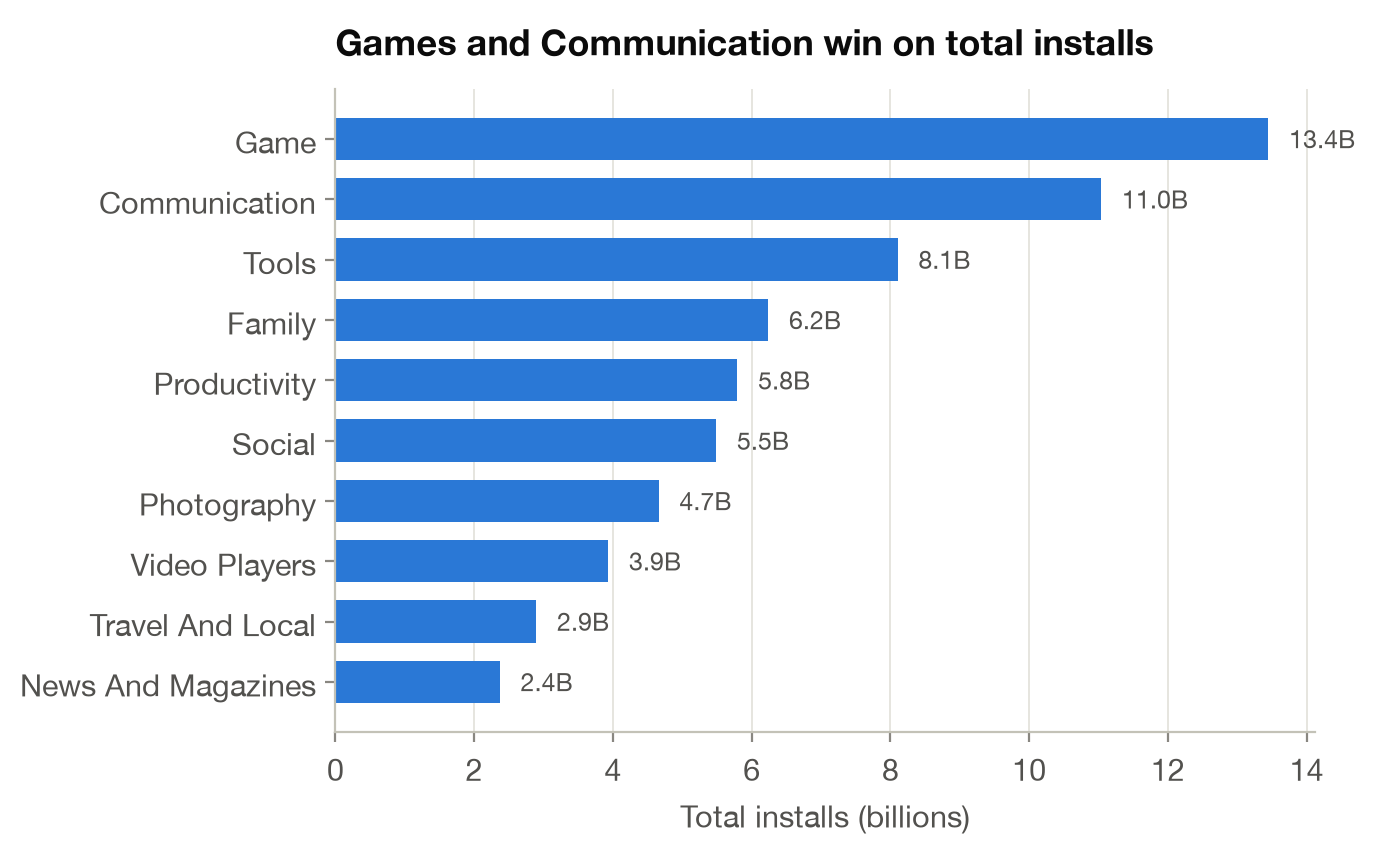
\includegraphics[width=0.49\linewidth]{ps_installs_by_category.png}\hfill
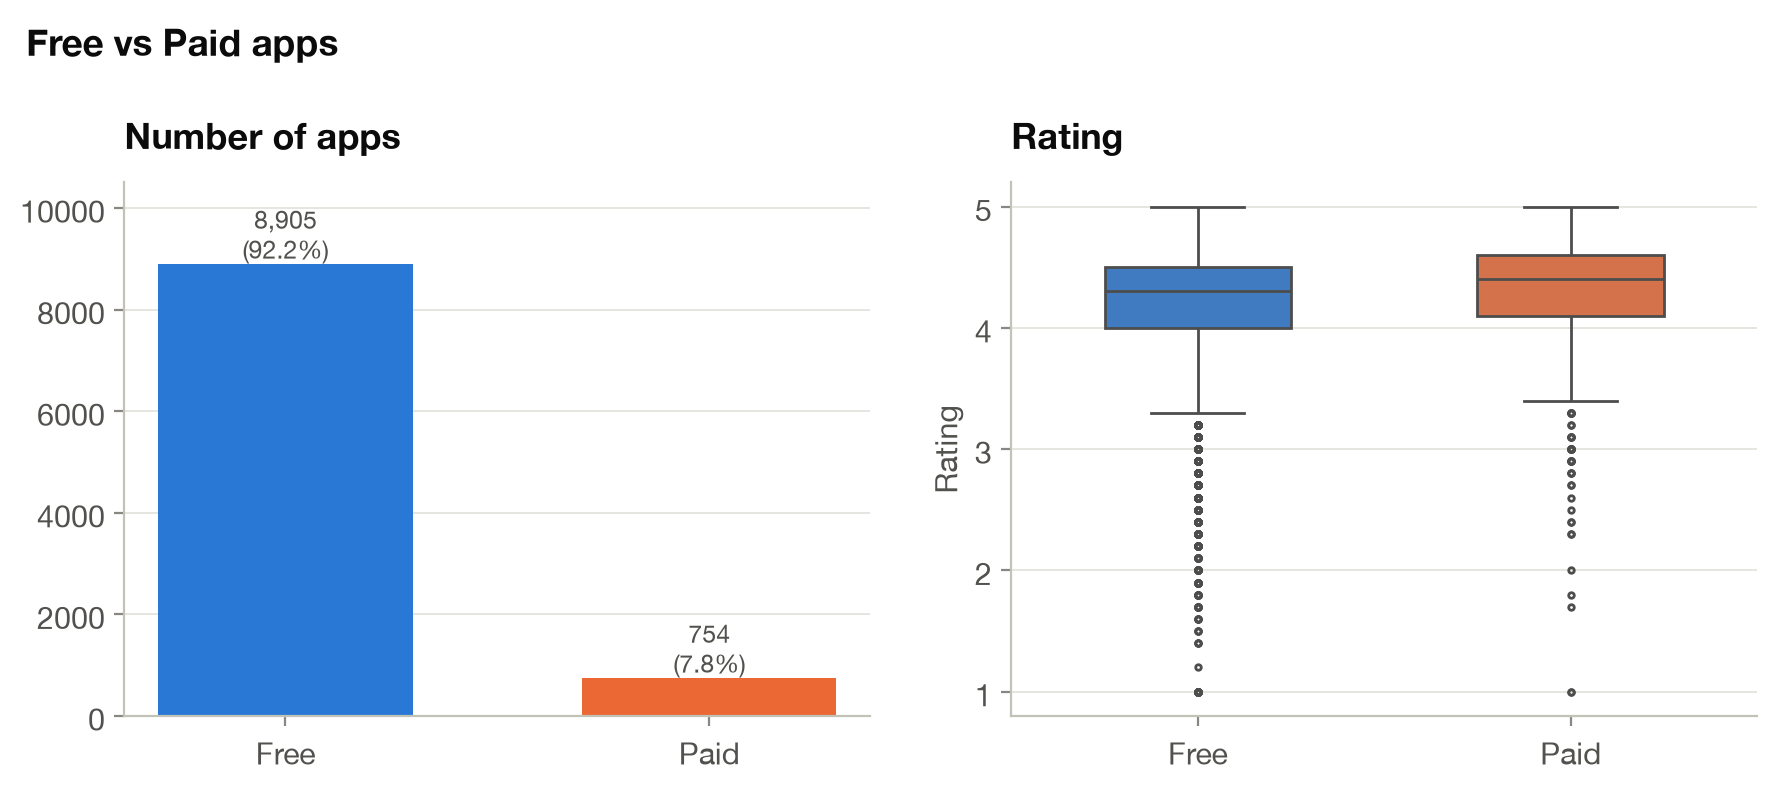
\includegraphics[width=0.49\linewidth]{ps_free_vs_paid.png}
\caption{Play Store: total installs by category (left) and free vs paid apps (right)}
\label{fig:ps}
\end{figure}
\textbf{Interpretation (Figure~\ref{fig:ps}).} Supply is not the same as demand. Family has the most apps (1,878), but
Game (13.4 billion installs) and Communication (11.0 billion) collect the most installs. Free apps are 92.2\% of the
store, and the median free app has 100,000 installs against 1,000 for a paid app. Paid apps are rated slightly higher
(4.26 vs 4.17). Ratings are inflated (median 4.3; 77\% of rated apps score $\ge$4.0). Reviews track installs almost
perfectly (Spearman $\rho=0.97$). Apps updated within the last month average 4.27 stars, against 4.05 for apps left
untouched for two years.

\begin{figure}[H]
\centering
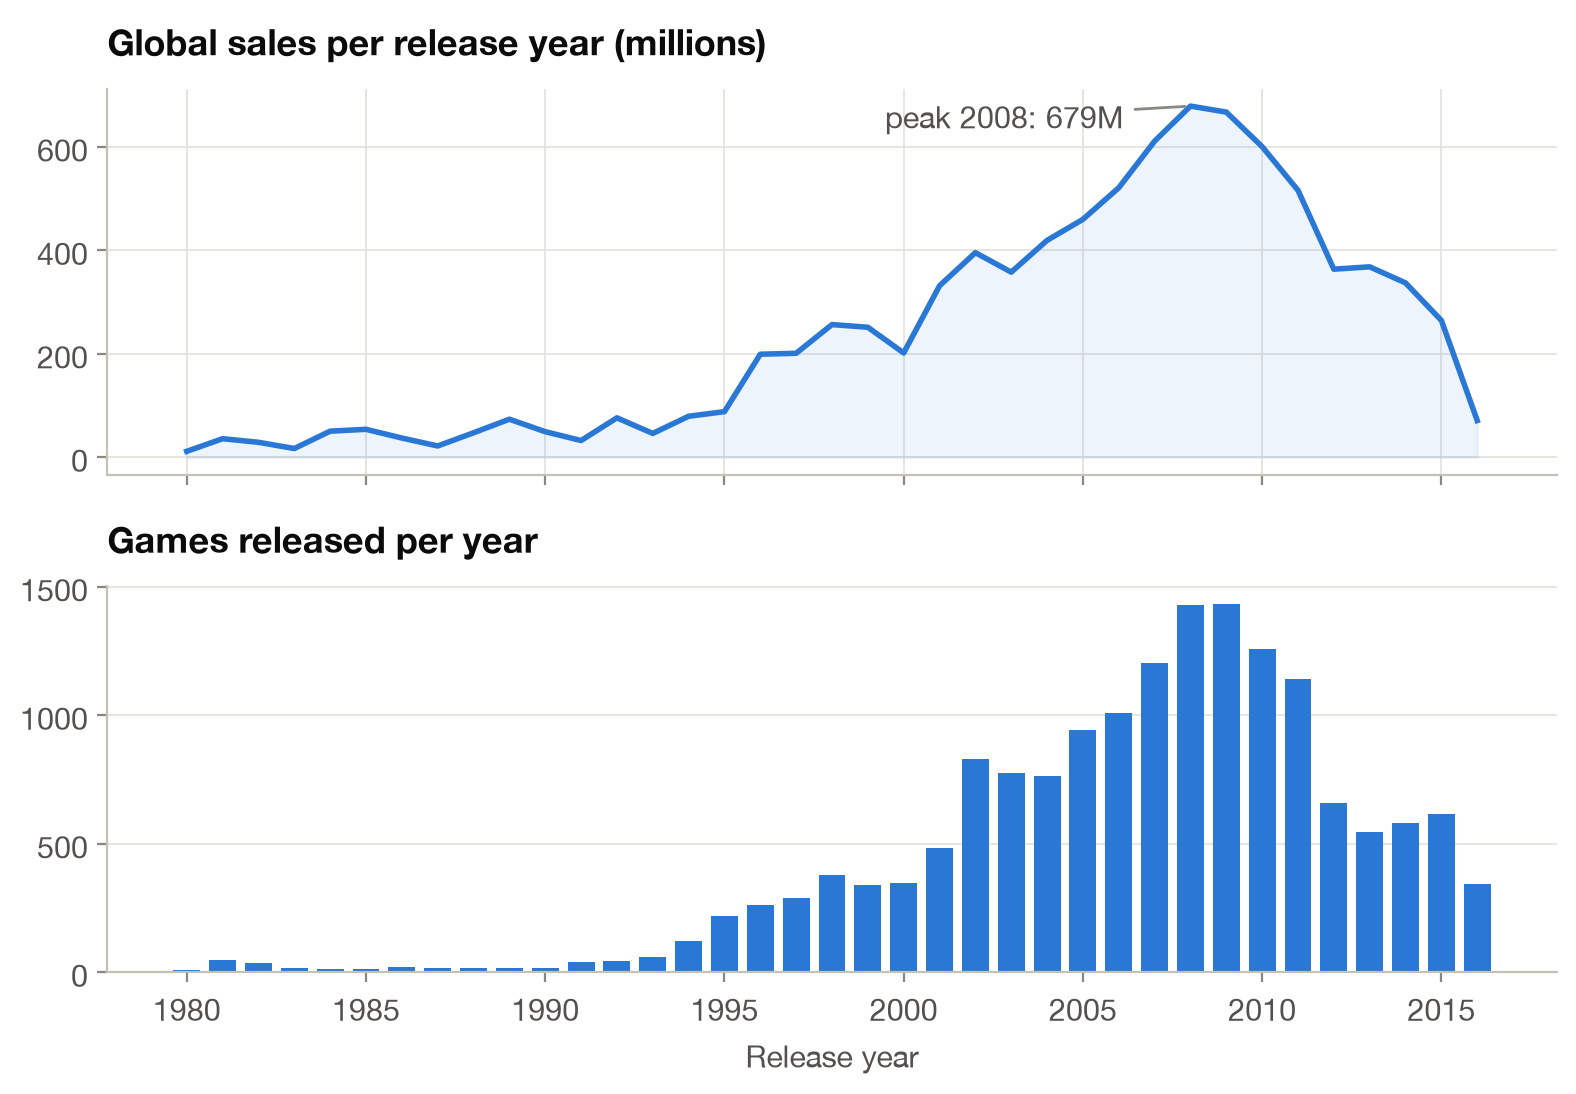
\includegraphics[width=0.49\linewidth]{vg_lifecycle.png}\hfill
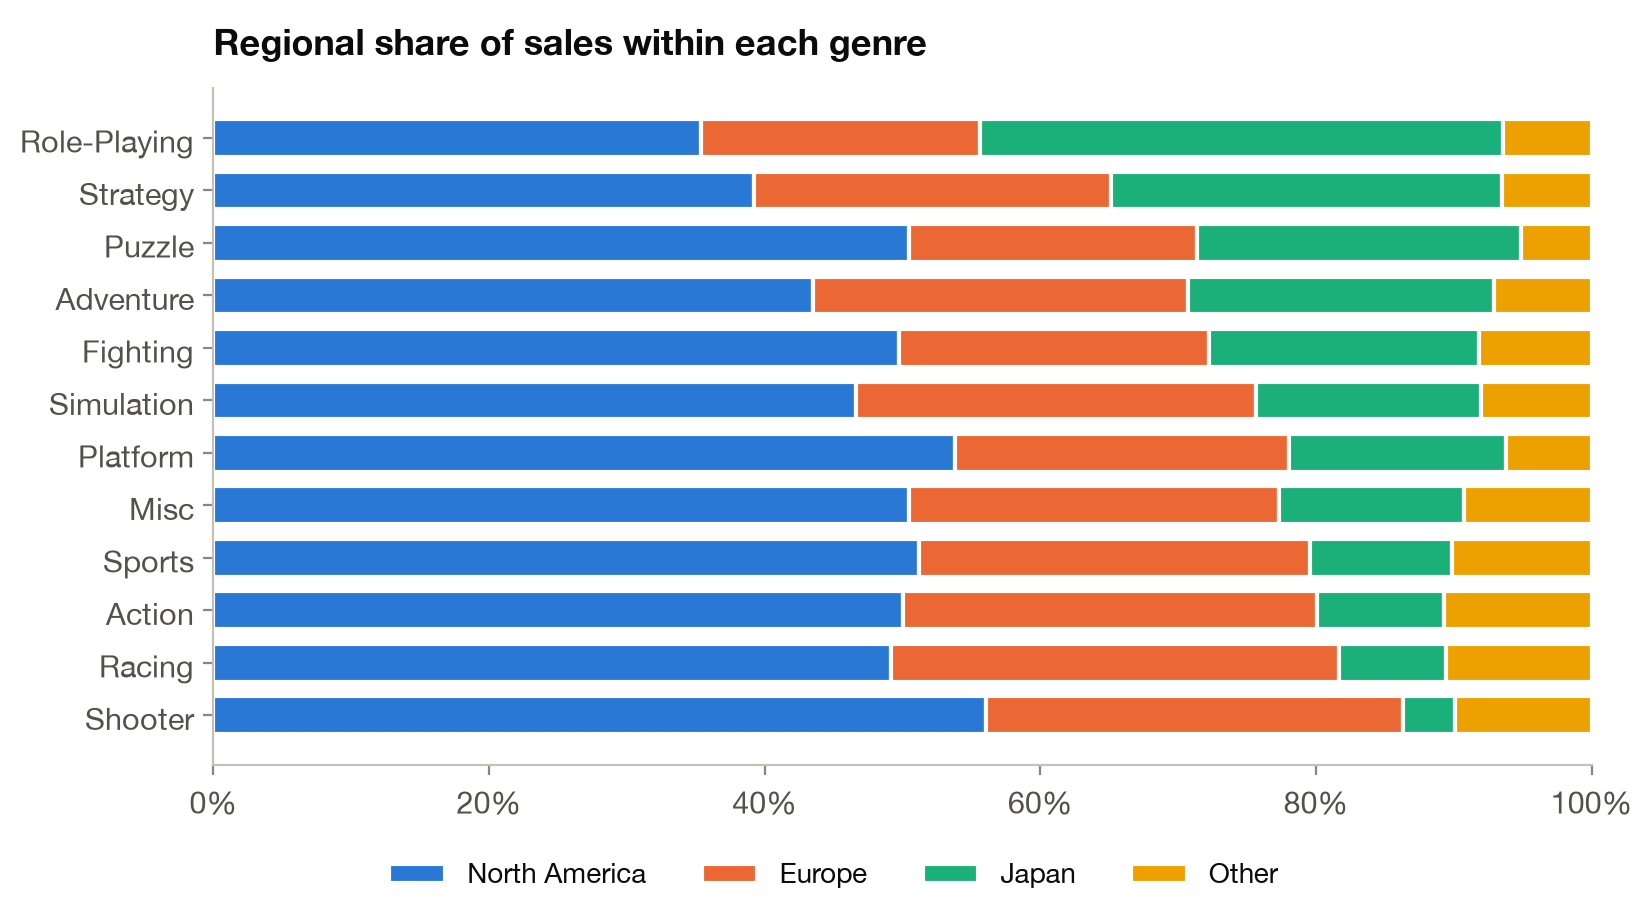
\includegraphics[width=0.49\linewidth]{vg_region_share_by_genre.png}
\caption{Video games: industry lifecycle 1980–2016 (left) and regional share of sales within each genre (right)}
\label{fig:vg}
\end{figure}
\textbf{Interpretation (Figure~\ref{fig:vg}).} The market is driven by hits. The median game sells 0.17 million copies,
while the top 1\% of games earn 21.1\% of all sales. Sales grew to a peak in 2008 (679 million units) and then declined;
the decline is partly real (the shift to digital and mobile) and partly an artefact of the data. North America accounts
for 49.1\% of sales, Europe 27.3\% and Japan 14.6\%. Japan behaves as a separate market: its sales correlate only 0.61
with global sales, against 0.94 for North America. Role-Playing is Japan's leading genre, and 38\% of all RPG sales are
Japanese.

\begin{figure}[H]
\centering
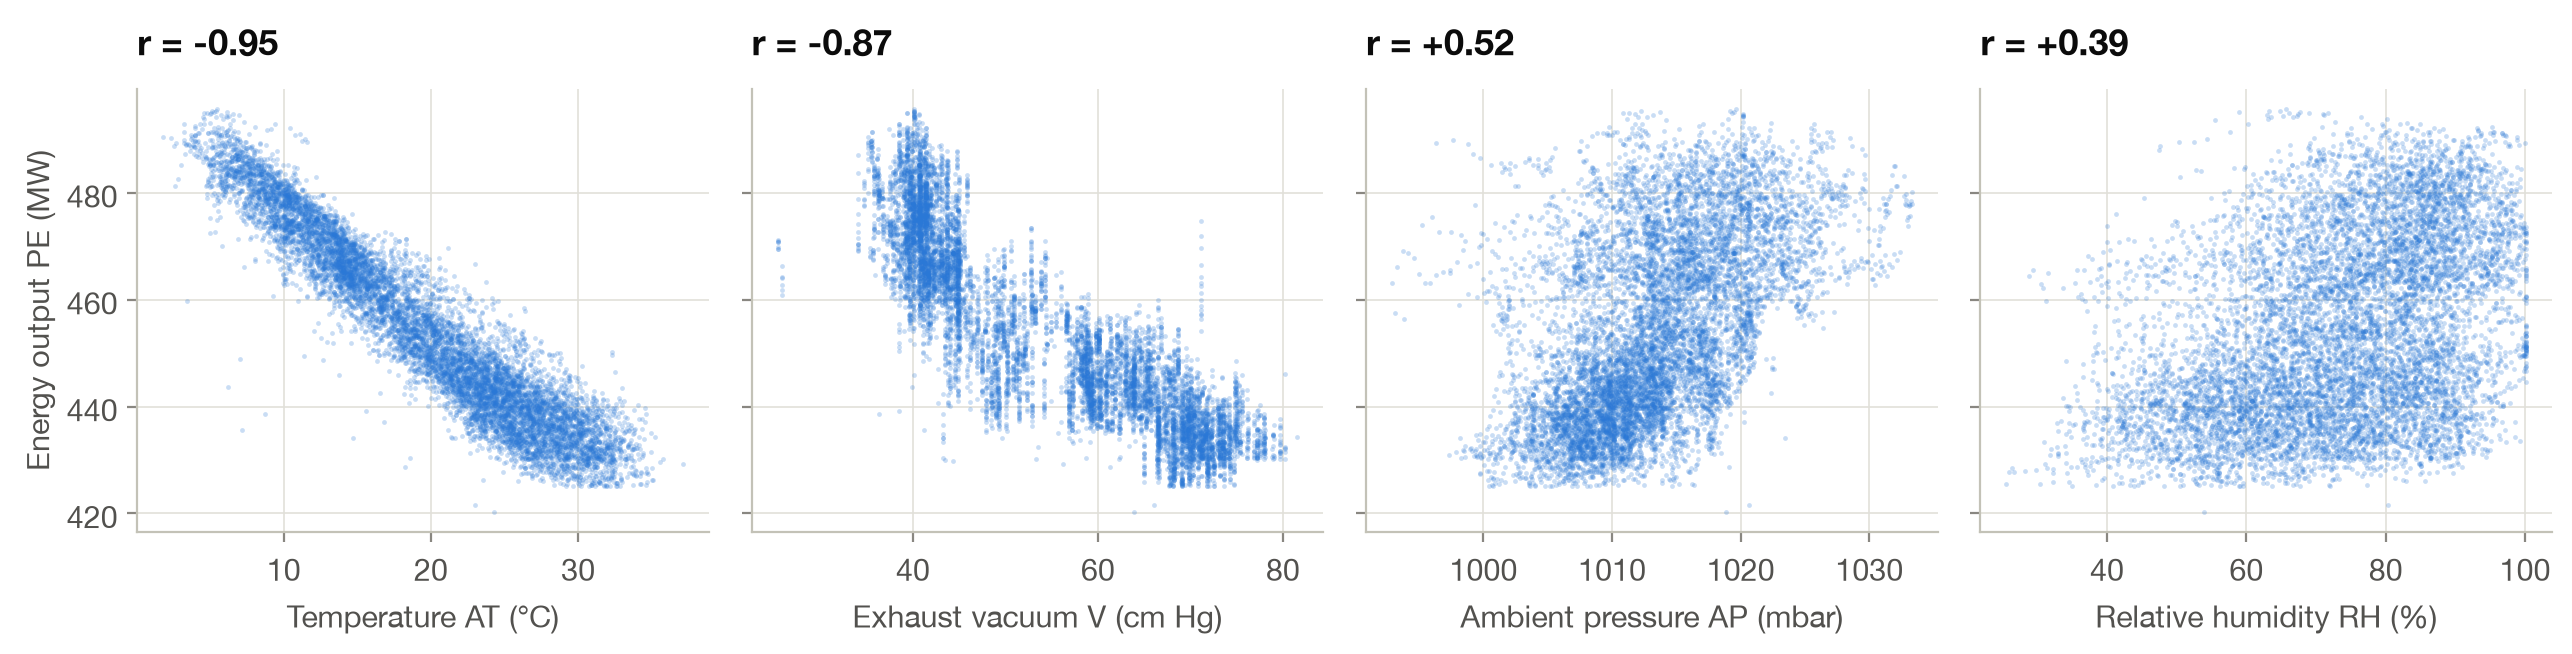
\includegraphics[width=\linewidth]{cc_feature_vs_target.png}
\caption{CCPP: each ambient feature against energy output PE, with Pearson correlation}
\label{fig:ccfeat}
\end{figure}
\textbf{Interpretation (Figure~\ref{fig:ccfeat}).} Temperature ($r=-0.95$) and exhaust vacuum ($r=-0.87$) are strong,
nearly linear negative drivers: hotter air is less dense, so the turbine produces less power. AT and V are correlated
with each other (variance inflation factors 6.0 and 3.9), which is moderate multicollinearity. The slight curvature of
the AT relationship suggests that non-linear models should help.

\begin{figure}[H]
\centering
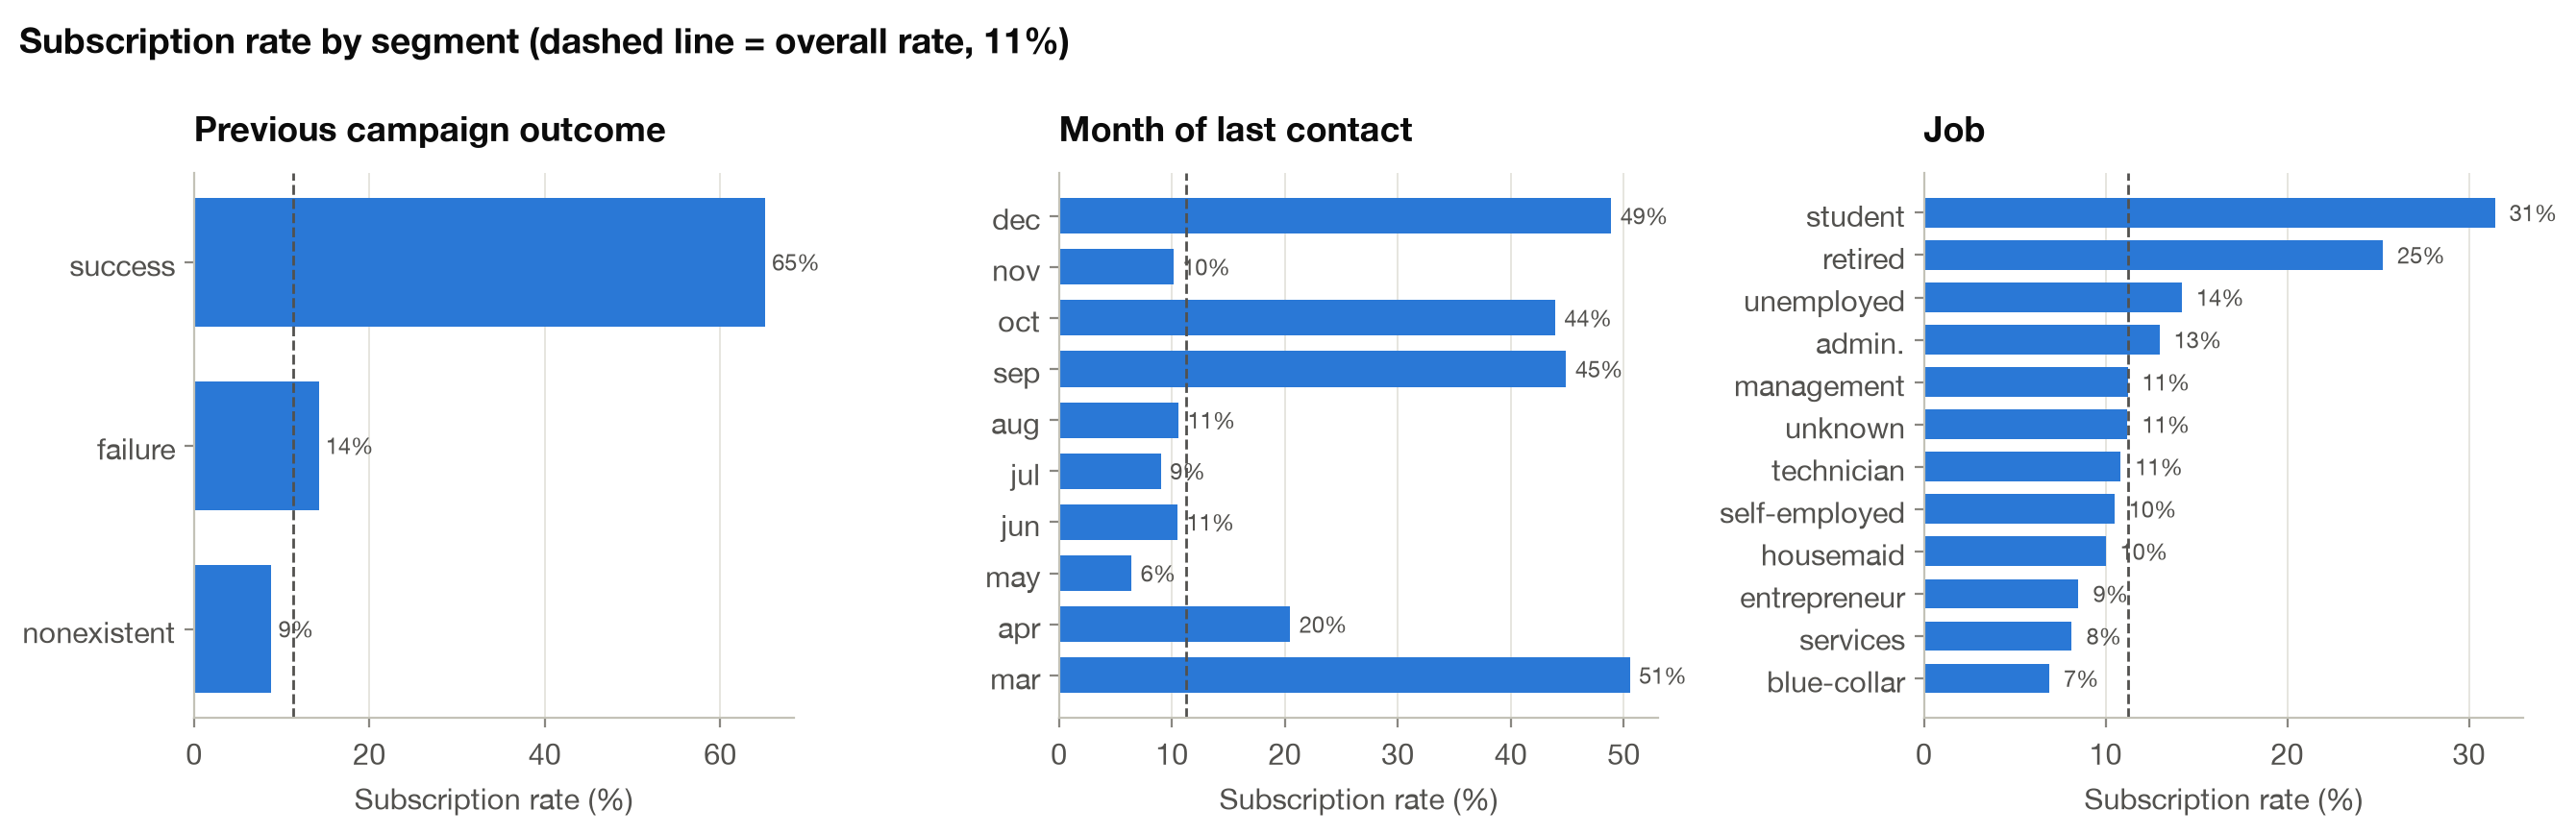
\includegraphics[width=\linewidth]{bk_rate_by_category.png}
\caption{Bank Marketing: subscription rate by previous-campaign outcome, month and job (dashed line = overall 11\%)}
\label{fig:bkrate}
\end{figure}
\textbf{Interpretation (Figure~\ref{fig:bkrate}).} Clients whose previous campaign succeeded subscribe 65\% of the
time. March, September, October and December convert at 44–51\% but are rarely used, while May has the most calls and
the lowest rate (6.4\%). Students (31\%) and retirees (25\%) are the most receptive groups.

\section{Proposed System Architecture / Workflow}
\begin{figure}[H]
\centering
\begin{tikzpicture}[node distance=0.45cm and 0.5cm, font=\small,
  box/.style={draw=navy, fill=lightblue, rounded corners=3pt, minimum height=1.1cm, text width=2.3cm, align=center},
  hl/.style={box, fill=lightorange, draw=accent}, arr/.style={-{Stealth[length=2.5mm]}, thick, navy}]
\node[box] (in) {Raw data\\(4 datasets)};
\node[box, right=of in] (aud) {Audit:\\types, duplicates, missing};
\node[box, right=of aud] (cl) {Cleaning \&\\feature engineering};
\node[box, right=of cl] (eda) {EDA \&\\insights (Unit 1)};
\node[box, below=1.1cm of cl] (split) {Train/test split\\(80/20, stratified)};
\node[box, left=of split] (pipe) {Pipeline: encode\\+ scale (train only)};
\node[hl, left=of pipe] (mod) {10+ models\\5-fold CV};
\node[box, right=of split] (tune) {Tuning \& threshold selection};
\node[hl, right=of tune] (eval) {Test-set evaluation\\\& interpretation};
\draw[arr] (in) -- (aud); \draw[arr] (aud) -- (cl); \draw[arr] (cl) -- (eda);
\draw[arr] (cl) -- (split); \draw[arr] (split) -- (pipe); \draw[arr] (pipe) -- (mod);
\draw[arr] (mod.south) |- ++(0,-0.5) -| (tune.south); \draw[arr] (tune) -- (eval);
\end{tikzpicture}
\caption{Workflow for Units 1 and 2}
\label{fig:wf12}
\end{figure}
Raw data is first audited (types, duplicates, missing values) and cleaned. The EDA branch (Unit 1) ends in insights.
The modelling branch (Unit 2) splits the data before any fitting. Encoding and scaling sit inside a pipeline so that
they are fitted on training folds only. More than ten models are compared with 5-fold cross-validation. The best family
is then tuned (GridSearchCV for regression; decision-threshold selection on out-of-fold predictions for classification),
and the held-out test set is used exactly once.

\section{Algorithm Theory and Mathematical Formulation}
\textbf{Linear regression} minimises the squared error; \textbf{Ridge} and \textbf{Lasso} add $L_2$ and $L_1$ penalties:
\begin{equation}
\hat{\boldsymbol\beta}=\arg\min_{\boldsymbol\beta}\ \sum_{i=1}^{n}\big(y_i-\mathbf{x}_i^\top\boldsymbol\beta\big)^2
+\lambda_2\lVert\boldsymbol\beta\rVert_2^2+\lambda_1\lVert\boldsymbol\beta\rVert_1 .
\end{equation}
\textbf{Logistic regression} models the probability of the positive class with the sigmoid and is fitted by minimising
the log-loss:
\begin{equation}
P(y=1\mid\mathbf{x})=\sigma(\mathbf{w}^\top\mathbf{x}+b)=\frac{1}{1+e^{-(\mathbf{w}^\top\mathbf{x}+b)}},\qquad
\mathcal{L}=-\sum_i\big[y_i\log p_i+(1-y_i)\log(1-p_i)\big].
\end{equation}
\textbf{Decision trees} split the data recursively to reduce impurity (Gini or variance). \textbf{Random Forest} averages
bootstrapped, decorrelated trees. \textbf{Gradient Boosting / XGBoost} \cite{friedman,xgboost} add trees sequentially, each one fitted to the
negative gradient of the loss (Chapter 4 covers these in depth). \textbf{KNN} predicts from the $k$ nearest neighbours,
and \textbf{SVR} fits an $\varepsilon$-insensitive tube in an RBF feature space. These methods follow \cite{esl,sklearn}. Class imbalance is handled by
class-weighting the loss (weight $\propto 1/\text{class frequency}$) or by SMOTE oversampling \cite{chawla} inside the CV folds.

\textbf{Evaluation metrics.}
\begin{equation}
\text{RMSE}=\sqrt{\tfrac{1}{n}\sum(y_i-\hat y_i)^2},\quad
\text{MAE}=\tfrac{1}{n}\sum|y_i-\hat y_i|,\quad
R^2=1-\frac{\sum(y_i-\hat y_i)^2}{\sum(y_i-\bar y)^2},
\end{equation}
\begin{equation}
\text{Precision}=\frac{TP}{TP+FP},\quad \text{Recall}=\frac{TP}{TP+FN},\quad
F_1=\frac{2\cdot\text{Precision}\cdot\text{Recall}}{\text{Precision}+\text{Recall}} .
\end{equation}
ROC-AUC is the probability that a randomly chosen positive is ranked above a randomly chosen negative. These methods are
appropriate because the CCPP relationships are smooth but slightly non-linear, which favours ensembles over linear
models. The bank data is imbalanced, which makes F1, recall and AUC the meaningful metrics and accuracy misleading.

\section{Results and Performance Evaluation}
\begin{table}[H]
\centering
\caption{CCPP regression: 5-fold CV and held-out test results (sorted by test RMSE)}
\label{tab:reg}
\begin{tabular}{@{}lcccc@{}}
\toprule
\textbf{Model} & \textbf{CV $R^2$} & \textbf{Test MAE (MW)} & \textbf{Test RMSE (MW)} & \textbf{Test $R^2$} \\
\midrule
\rowcolor{lightorange} XGBoost (tuned) & 0.9670 & 2.166 & \textbf{3.171} & \textbf{0.9658} \\
XGBoost & 0.9656 & 2.287 & 3.282 & 0.9633 \\
Gradient Boosting & 0.9623 & 2.441 & 3.404 & 0.9606 \\
Random Forest & 0.9598 & 2.409 & 3.434 & 0.9599 \\
KNN ($k=7$) & 0.9510 & 2.651 & 3.750 & 0.9521 \\
Decision Tree & 0.9417 & 2.933 & 4.075 & 0.9435 \\
SVR (RBF) & 0.9444 & 3.006 & 4.077 & 0.9434 \\
Polynomial (degree 3) & 0.9404 & 3.269 & 4.234 & 0.9390 \\
Lasso / Ridge & 0.9283 & 3.621 & 4.587 & 0.9284 \\
Linear Regression & 0.9283 & 3.621 & 4.587 & 0.9284 \\
\bottomrule
\end{tabular}
\end{table}
\begin{figure}[H]
\centering
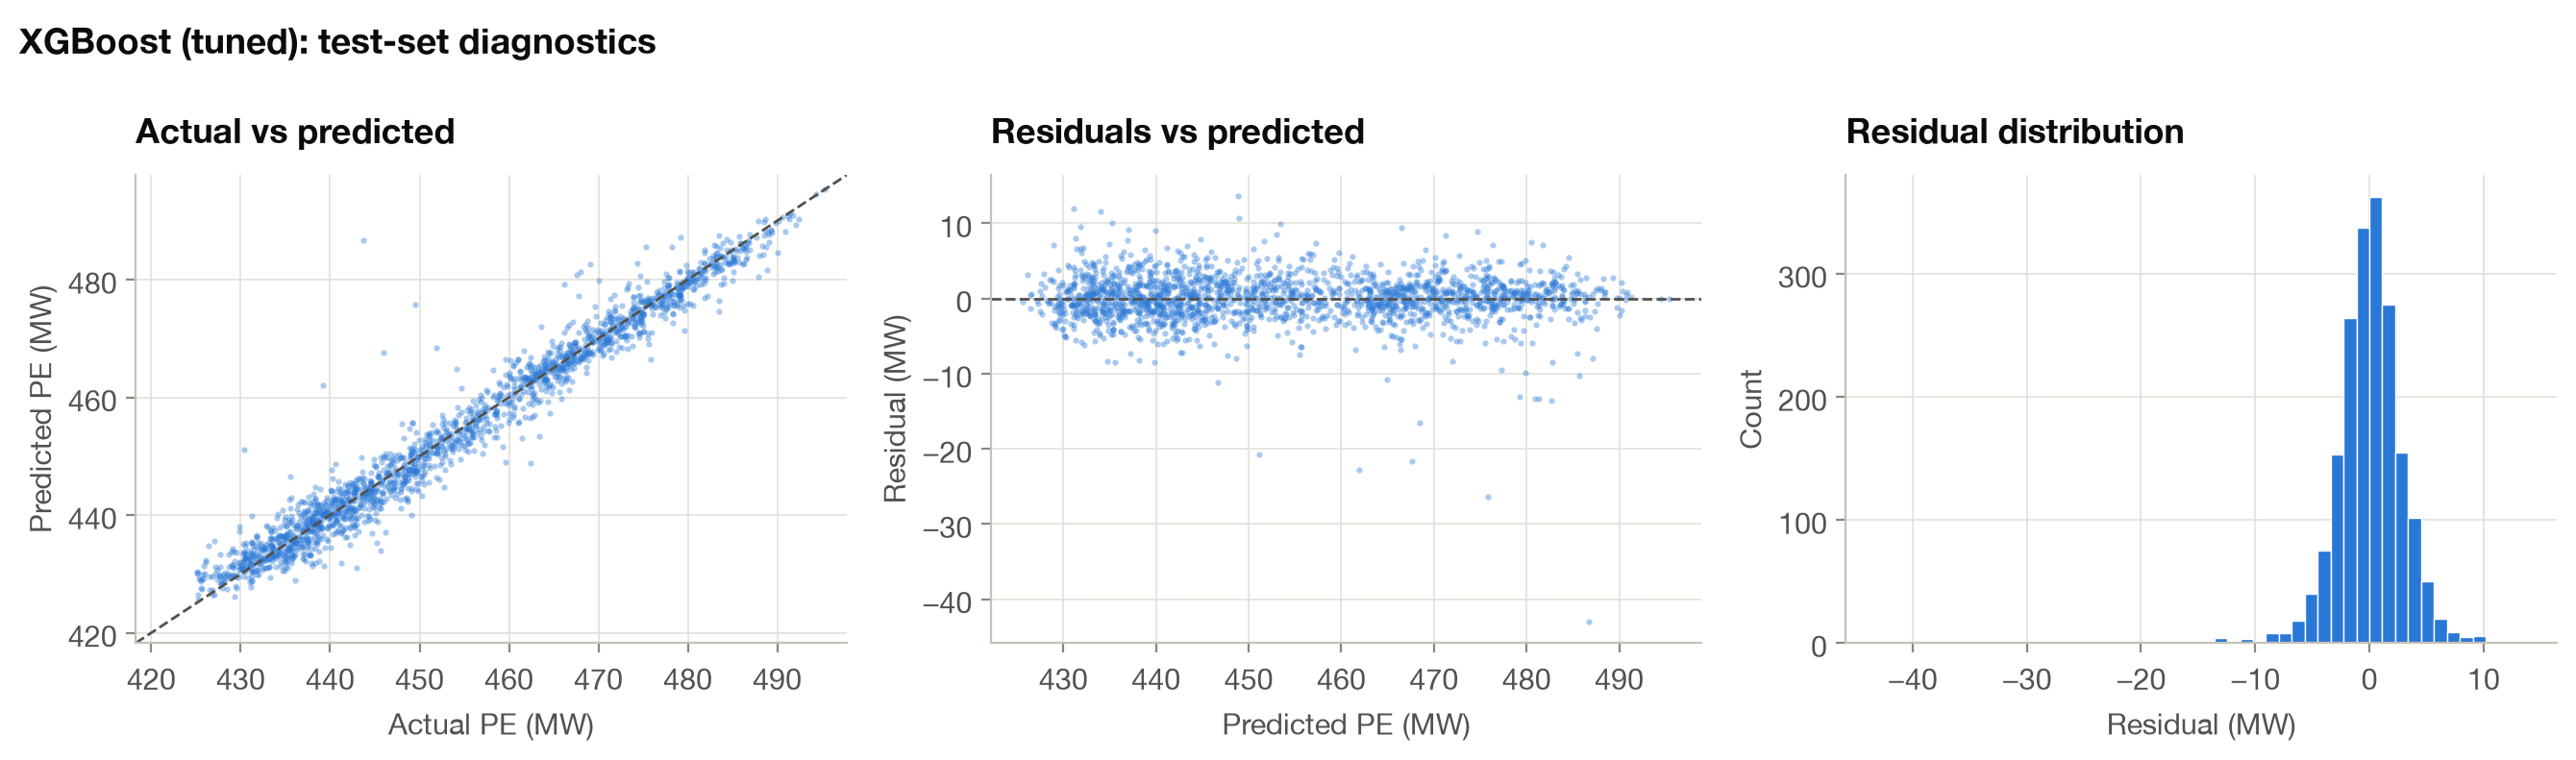
\includegraphics[width=\linewidth]{cc_best_diagnostics.png}
\caption{CCPP: tuned XGBoost test-set diagnostics (actual vs predicted, residuals, residual distribution)}
\label{fig:ccdiag}
\end{figure}
\textbf{Interpretation (Table~\ref{tab:reg}, Figure~\ref{fig:ccdiag}).} The tuned XGBoost model (1,200 trees, learning
rate 0.03, depth 7) has RMSE 3.17 MW and $R^2$ 0.966, which is \textbf{30.9\% lower error} than linear regression
(4.59 MW). 92.5\% of hourly predictions fall within $\pm$5 MW. Residuals are centred at zero with no pattern, so the
model shows no systematic bias. Ridge and Lasso match plain linear regression: with four features there is nothing to
regularise. CV $R^2$ agrees with test $R^2$ (standard deviation 0.003), so the ranking is stable. Permutation importance
confirms that temperature dominates.

\begin{table}[H]
\centering
\caption{Bank Marketing classification: held-out test results (sorted by F1)}
\label{tab:clf}
\begin{tabular}{@{}lccccc@{}}
\toprule
\textbf{Model} & \textbf{Accuracy} & \textbf{Recall} & \textbf{F1} & \textbf{ROC-AUC} & \textbf{PR-AUC} \\
\midrule
\rowcolor{lightorange} XGBoost (weighted, threshold 0.65) & 0.881 & 0.595 & \textbf{0.531} & \textbf{0.812} & 0.484 \\
Random Forest (balanced) & 0.873 & 0.617 & 0.523 & 0.807 & 0.484 \\
XGBoost (weighted, threshold 0.50) & 0.845 & 0.654 & 0.487 & 0.812 & 0.484 \\
Decision Tree (balanced) & 0.847 & 0.637 & 0.484 & 0.801 & 0.460 \\
Logistic Reg. (balanced) & 0.831 & 0.645 & 0.462 & 0.800 & 0.446 \\
Logistic Reg. + SMOTE & 0.822 & 0.654 & 0.453 & 0.799 & 0.445 \\
Naive Bayes & 0.808 & 0.624 & 0.423 & 0.776 & 0.359 \\
KNN ($k=15$) & 0.898 & 0.263 & 0.368 & 0.773 & 0.419 \\
Gradient Boosting & 0.899 & 0.233 & 0.342 & 0.811 & 0.480 \\
Logistic Regression & 0.898 & 0.212 & 0.320 & 0.801 & 0.453 \\
Baseline (always ``no'') & 0.887 & 0.000 & 0.000 & 0.500 & 0.113 \\
\bottomrule
\end{tabular}
\end{table}
\begin{figure}[H]
\centering
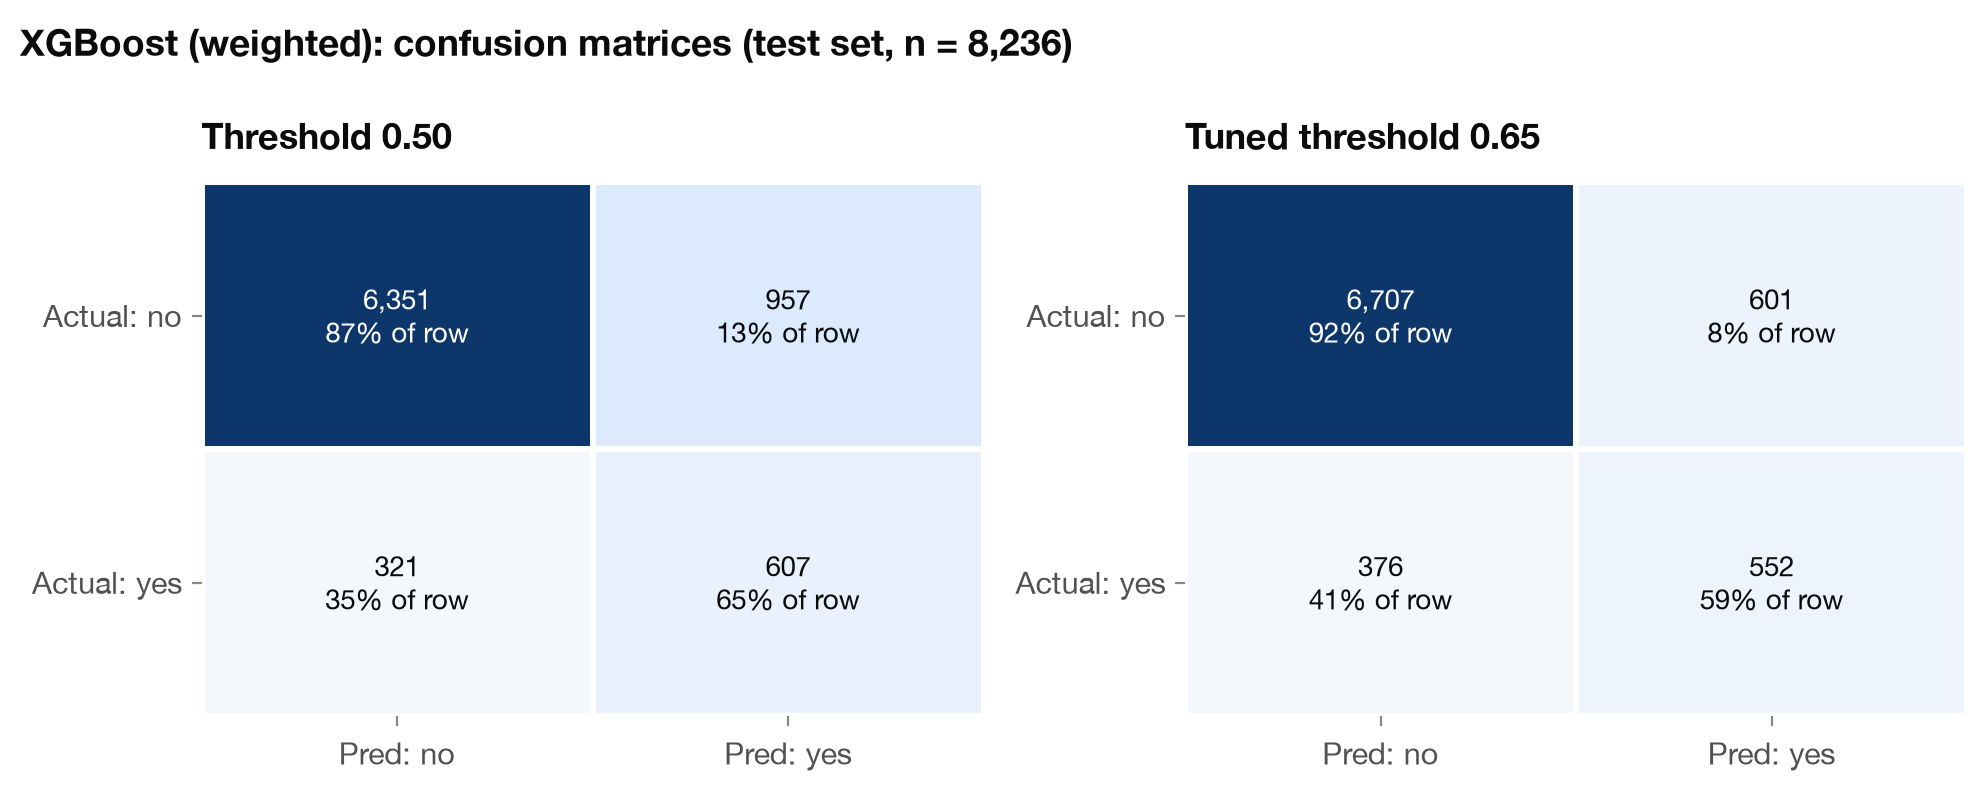
\includegraphics[width=0.52\linewidth]{bk_confusion.png}\hfill
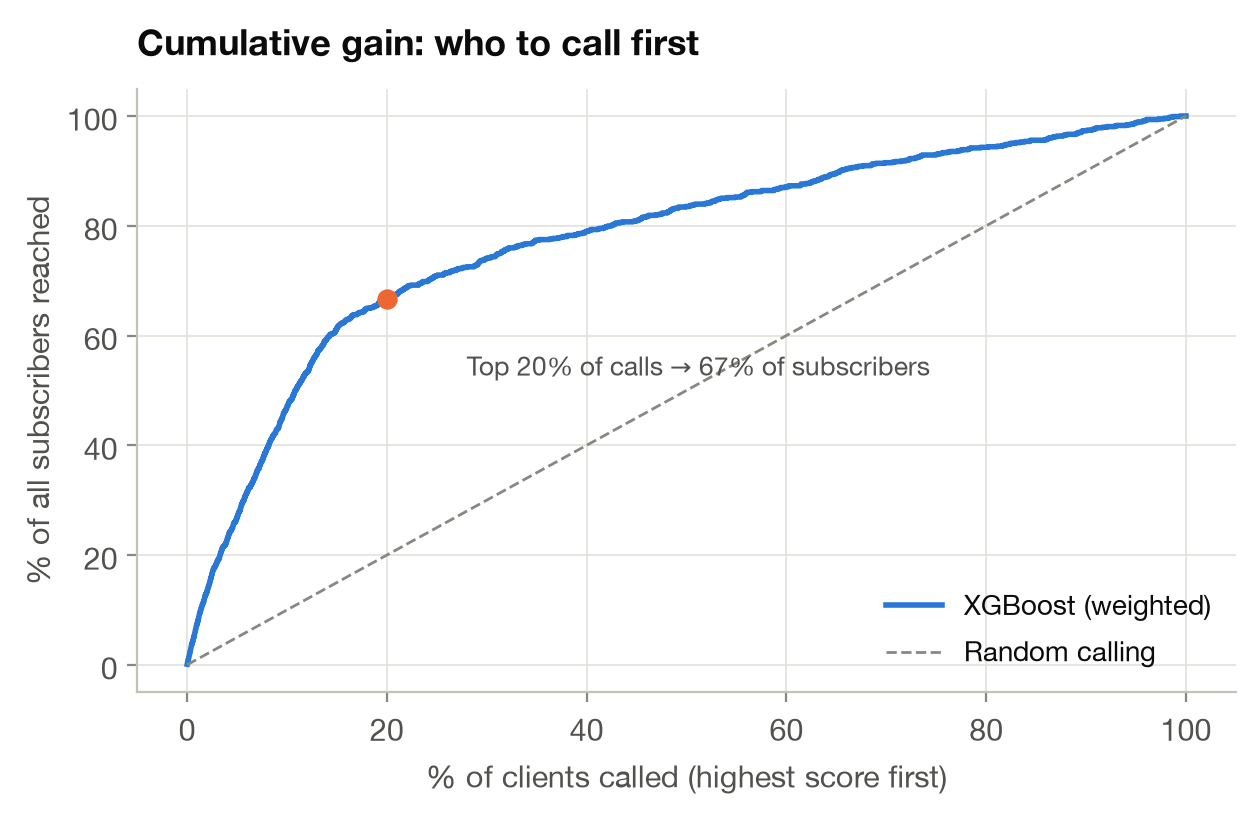
\includegraphics[width=0.46\linewidth]{bk_gain_curve.png}
\caption{Bank Marketing: confusion matrices at thresholds 0.50 and 0.65 (left), and cumulative gain (right)}
\label{fig:bk}
\end{figure}
\textbf{Interpretation (Table~\ref{tab:clf}, Figure~\ref{fig:bk}).} The \emph{accuracy trap} is clear: a model that
always predicts ``no'' is 88.7\% accurate but finds no subscribers, and plain logistic regression finds only 21\% of them.
Class weighting or SMOTE roughly triples recall at the same ROC-AUC. Class-weighted XGBoost with the F1-optimal threshold
(0.65, chosen on out-of-fold training predictions) is the best model (F1 0.531, ROC-AUC 0.812). Raising the threshold
from 0.50 to 0.65 cuts wasted calls from 957 to 601 (37\% fewer). Calling the top 20\% of clients ranked by the model
reaches 66.7\% of all subscribers, a \textbf{3.3$\times$ lift} over random calling.

\section{Discussion and Findings}
\begin{itemize}
\item \textbf{What worked:} tree ensembles (XGBoost, Random Forest) were the best models on both supervised tasks.
Pipelines prevented preprocessing leakage, and threshold tuning on out-of-fold predictions turned a good ranking model
into a useful decision rule.
\item \textbf{Challenges:} data quality dominated the EDA effort (text-encoded numbers, duplicates, informative
missingness). On the bank data, finding and removing the leaking \texttt{duration} feature was essential for a realistic
model. With it, published models report AUC above 0.9, which overstates what can be known before a call.
\item \textbf{Limitations:} the CCPP models used default settings except for XGBoost. The bank model's ROC-AUC ceiling of
about 0.81 reflects the limited information available before a call, and its macro-economic features are specific to
2008–2010.
\end{itemize}

\section{Chapter Conclusion}
PBL I delivered quantified market insights (Unit 1) and two well-validated supervised models (Unit 2): CCPP regression
with RMSE 3.17 MW ($R^2$ 0.966), and bank-marketing classification with F1 0.531, ROC-AUC 0.812 and a 3.3$\times$ lift.
These results set the baseline methodology used in the later chapters: audit-first cleaning, leakage-free pipelines,
cross-validated model comparison, metrics matched to the class balance, and a single use of the test set. They also
showed that gradient-boosted tree ensembles are strong on tabular data, a finding Chapter 4 tests directly.

\chapter{Unsupervised Learning and Sequential Data Modelling – (Units 3 and 4)}

\section{Overview of Allotted Unit 3 and Unit 4 Topics}
Group 10's PBL II topic is \textbf{Sequential Human Activity Recognition}. The allotted algorithms are Markov models,
Hidden Markov Models (HMM), the forward–backward algorithm and the Viterbi algorithm. The objective is to infer
activity-state sequences from accelerometer time series.
\begin{itemize}
\item \textbf{Unit 3 (clustering and dimensionality reduction):} K-Means and Gaussian Mixture Model (GMM) clustering of
per-window accelerometer features, with PCA for visualisation. Clustering groups windows by similarity and ignores time
order, so it is the natural non-sequential baseline for the HMM.
\item \textbf{Unit 4 (sequential modelling):} a Gaussian HMM trained without labels (Baum–Welch), hand-implemented
forward–backward and Viterbi algorithms, and a supervised (hybrid) HMM that decodes the activity sequences of unseen
people.
\end{itemize}

\section{Unit 3 – Dataset Description and Preprocessing}
A new dataset is used for PBL II: the \textbf{UCI Human Activity Recognition Using Smartphones} dataset (UCI ML
Repository \#240) \cite{anguita}. Thirty volunteers aged 19–48 performed six activities (Walking, Walking
Upstairs, Walking Downstairs, Sitting, Standing, Laying) with a Samsung Galaxy S II worn on the waist.
\begin{itemize}
\item \textbf{Signal:} the triaxial accelerometer was sampled at \textbf{50 Hz}. The dataset authors pre-filtered the
signals and segmented them into \textbf{2.56 s windows} (128 samples) with 50\% overlap, giving \textbf{10,299 windows}.
\item \textbf{Size and balance:} classes are roughly balanced (Laying 1,944, Standing 1,906, Sitting 1,777,
Walking 1,722, Upstairs 1,544, Downstairs 1,406 windows). There are no missing values.
\item \textbf{Relevance:} the labels exist, but the unsupervised methods never use them for training; they serve only to
measure how well the hidden structure is recovered.
\end{itemize}
\textbf{Feature engineering.} Each window's raw signal ($128\times3$ total acceleration) is summarised into 10 features:
\begin{itemize}
\item the mean and standard deviation of the acceleration magnitude $\lVert\mathbf a\rVert$, and its energy;
\item the per-axis means (the direction of gravity, which encodes the phone's orientation);
\item the per-axis standard deviations;
\item the jerk energy (mean squared sample-to-sample difference).
\end{itemize}
Features are standardised with a scaler fitted on training subjects only.

\textbf{Split by person.} The data is split by subject: 24 subjects (8,013 windows) for training and 6 unseen subjects
(2,286 windows) for testing. Windows from the same person never appear in both sets.

\section{Unit 3 – Theory, EDA, Implementation and Results}
\begin{figure}[H]
\centering
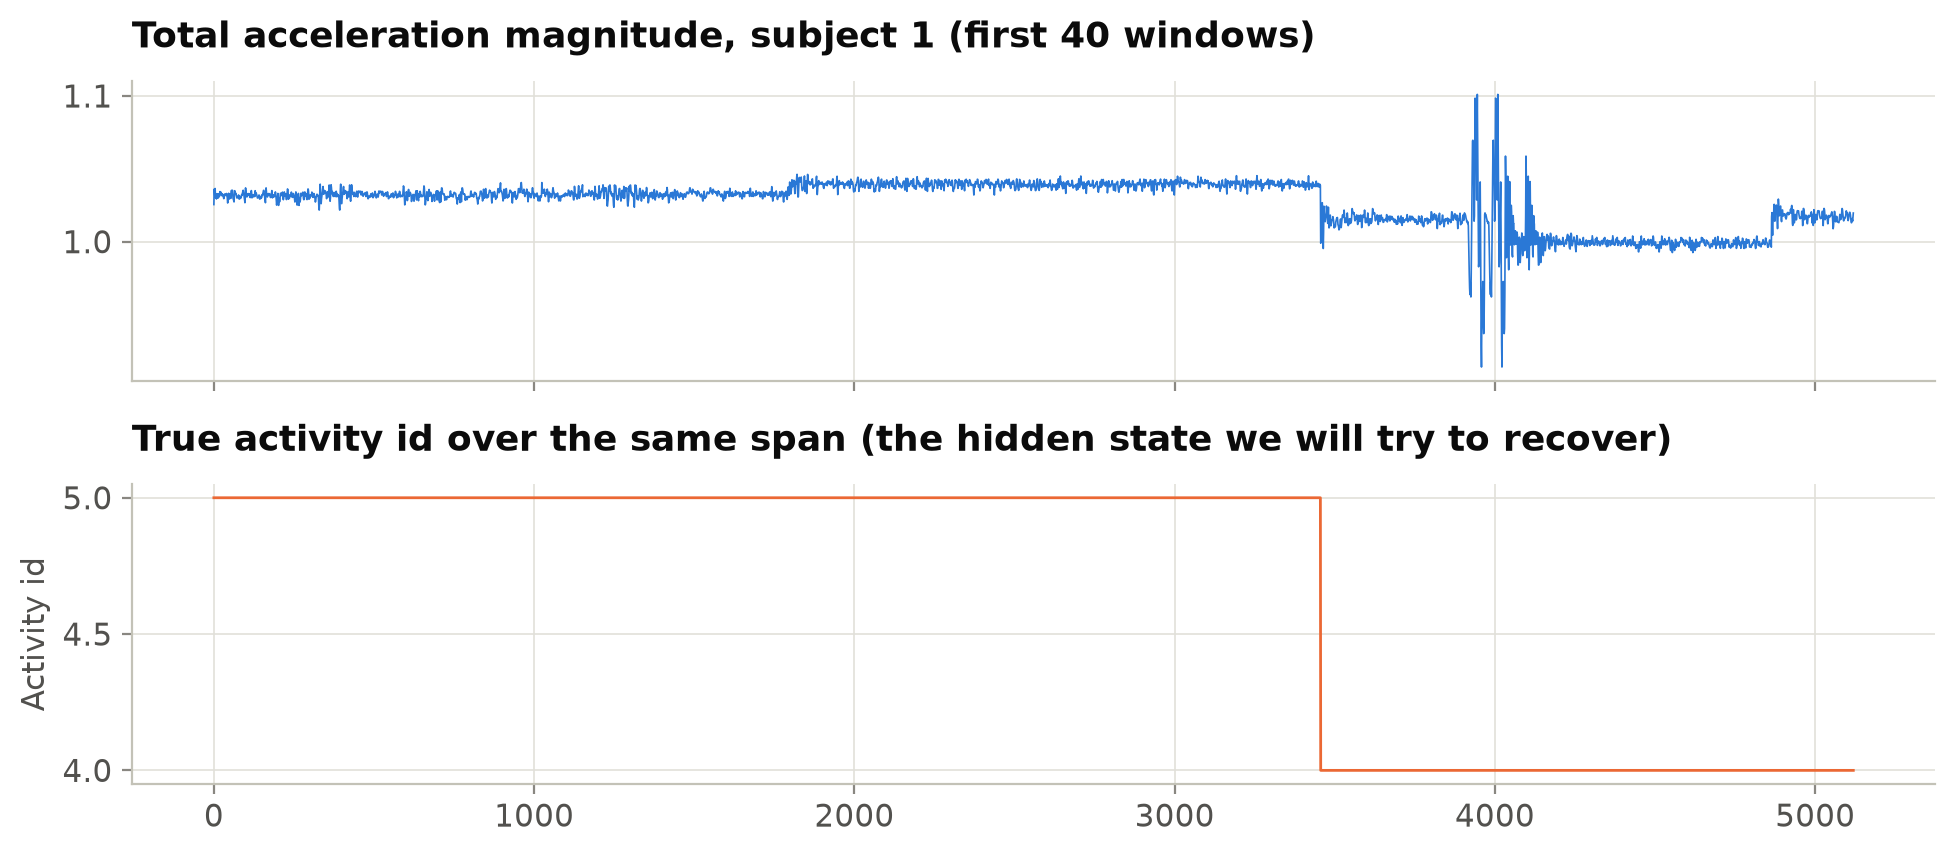
\includegraphics[width=0.53\linewidth]{har_signal_and_activity.png}\hfill
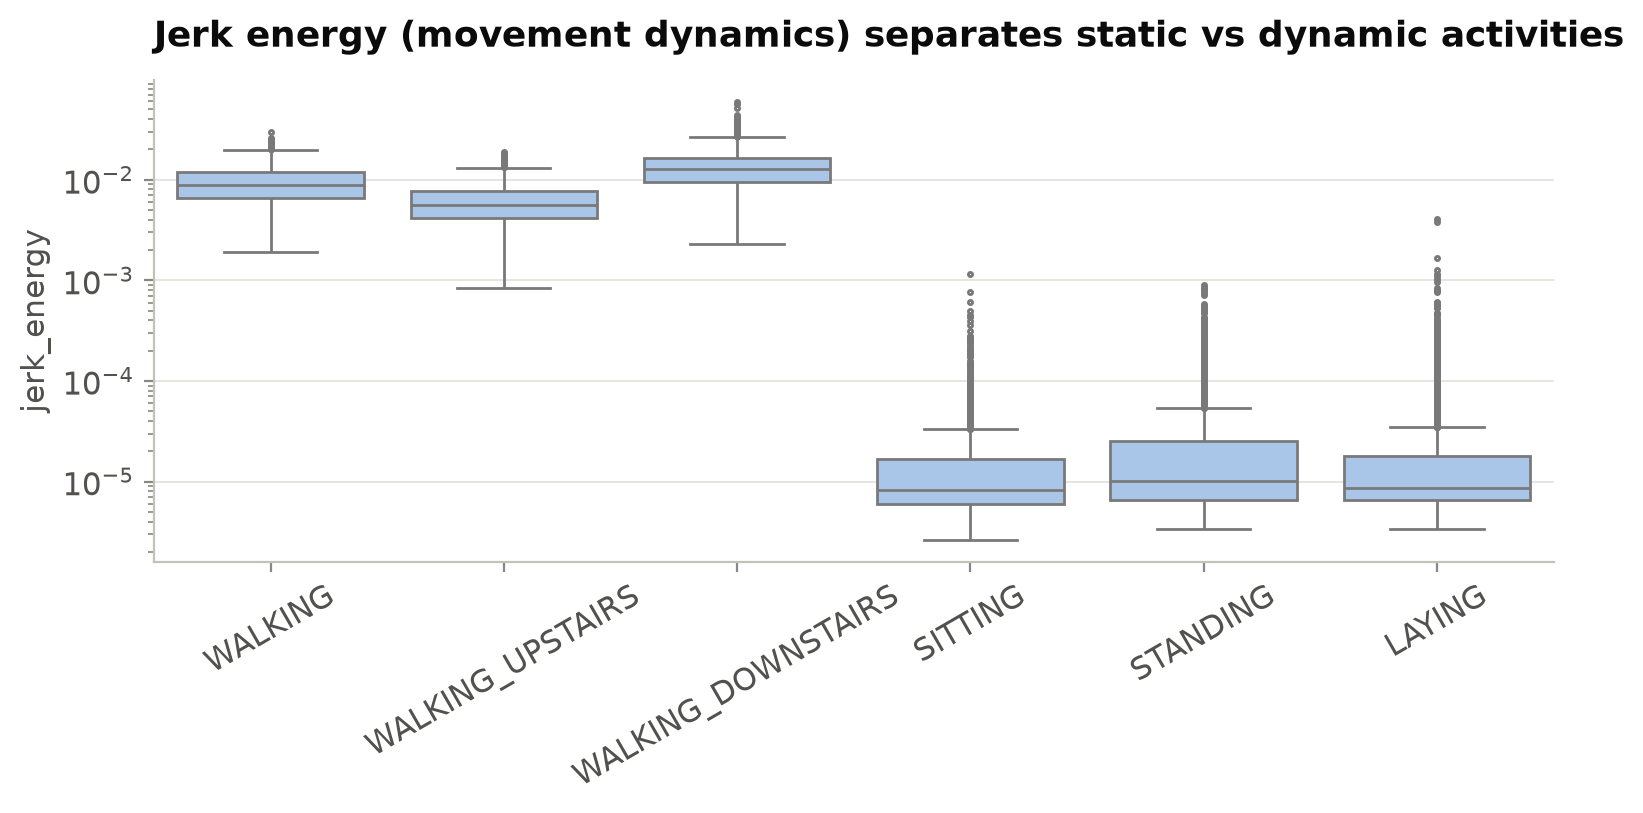
\includegraphics[width=0.45\linewidth]{har_jerk_by_activity.png}
\caption{HAR: acceleration magnitude and true activity for one subject (left); jerk energy by activity on a log scale (right)}
\label{fig:hareda}
\end{figure}
\textbf{Interpretation (Figure~\ref{fig:hareda}).} The acceleration magnitude stays near 1\,g (gravity) and is stable
while the activity is constant. It changes sharply when the activity switches: the burst near sample 3,500 is the act
of sitting down. Jerk energy separates \emph{dynamic} activities (about $10^{-2}$) from \emph{static} ones (about
$10^{-5}$), a thousand-fold gap. Within each group, however, the distributions overlap: Sitting, Standing and Laying look
alike, and so do the three walking types. The true activity is piecewise-constant, lasting on average
\textbf{29.5 windows ($\approx$38 s)} per bout. This persistence is the evidence for the Markov assumption.

\begin{figure}[H]
\centering
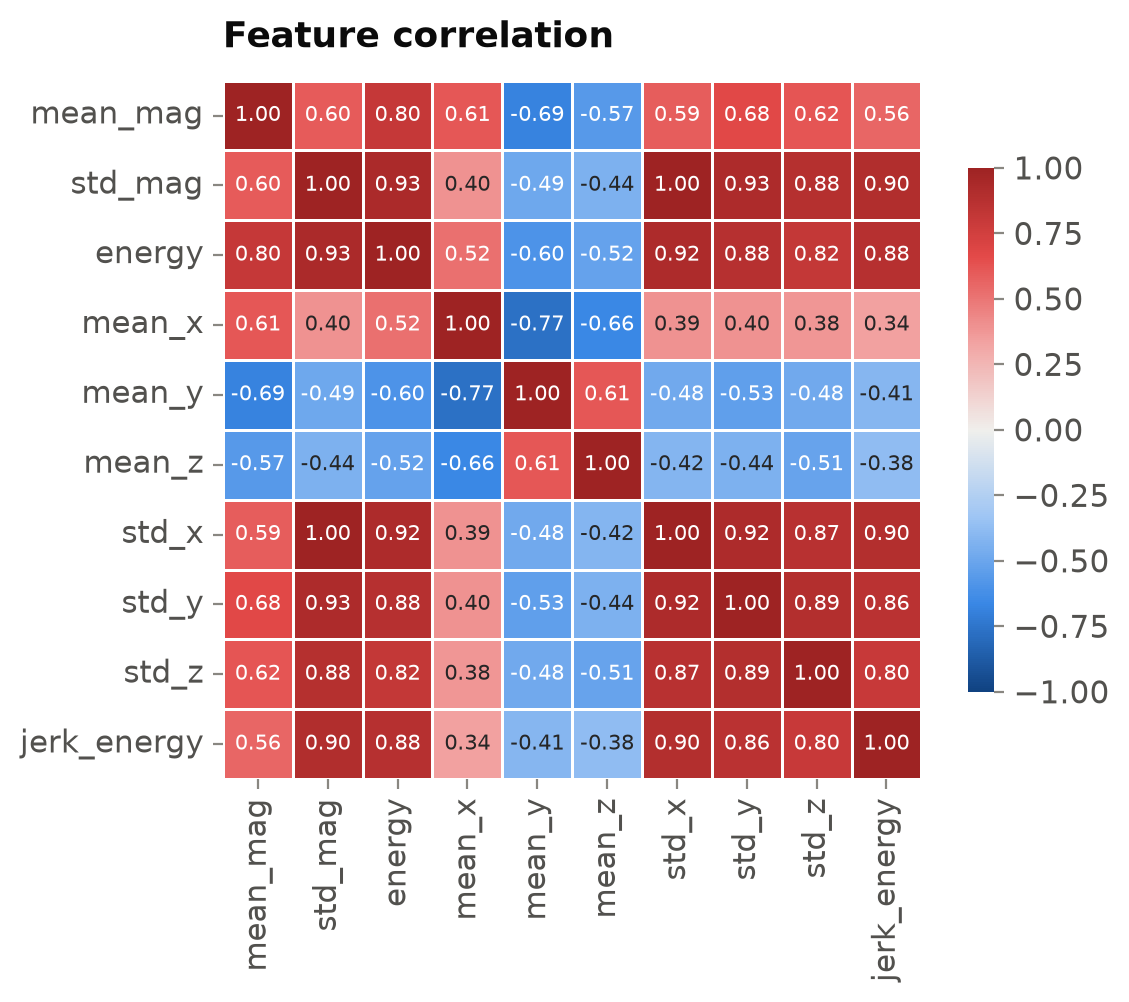
\includegraphics[width=0.62\linewidth]{har_feature_correlation.png}
\caption{Correlation between the ten engineered window features}
\label{fig:harcorr}
\end{figure}
\textbf{Interpretation (Figure~\ref{fig:harcorr}).} Magnitude statistics and per-axis standard deviations are strongly
correlated, so a few directions carry most of the information. This supports full-covariance Gaussian models (GMM and
HMM emissions), which capture the correlations, and a 2-D PCA projection for visualisation.

\section{Unit 3 – Algorithm Theory and Mathematical Formulation}
\textbf{K-Means} \cite{lloyd} partitions the windows $\{\mathbf x_i\}$ into $K$ clusters by minimising the within-cluster sum of
squares, alternating assignment and centroid update:
\begin{equation}
\min_{\{C_k\},\{\boldsymbol\mu_k\}}\ \sum_{k=1}^{K}\sum_{\mathbf x_i\in C_k}\lVert\mathbf x_i-\boldsymbol\mu_k\rVert^2 .
\end{equation}
\textbf{The Gaussian Mixture Model} is a soft, probabilistic generalisation fitted by Expectation–Maximisation \cite{dempster}:
\begin{equation}
p(\mathbf x)=\sum_{k=1}^{K}\pi_k\,\mathcal N(\mathbf x\mid\boldsymbol\mu_k,\boldsymbol\Sigma_k),\qquad
r_{ik}=\frac{\pi_k\,\mathcal N(\mathbf x_i\mid\boldsymbol\mu_k,\boldsymbol\Sigma_k)}{\sum_j\pi_j\,\mathcal N(\mathbf x_i\mid\boldsymbol\mu_j,\boldsymbol\Sigma_j)} .
\end{equation}
\textbf{PCA} projects the data onto the eigenvectors of its covariance matrix with the largest eigenvalues; it is used
only for 2-D visualisation. \textbf{Settings:} $K=6$ (one cluster per activity), K-Means with 10 restarts, GMM with full
covariances and 5 restarts. Clusters carry no names, so each cluster id is matched one-to-one to an activity by the
\textbf{Hungarian algorithm} \cite{kuhn} on the training confusion matrix, then applied unchanged to the test subjects.
\textbf{Metrics:} accuracy after matching; the Adjusted Rand Index (ARI, which needs no matching); the silhouette score;
and the average segment length (how many consecutive windows keep the same label).

\section{Unit 3 Proposed System Architecture / Workflow}
\begin{figure}[H]
\centering
\begin{tikzpicture}[node distance=0.4cm and 0.45cm, font=\small,
  box/.style={draw=navy, fill=lightblue, rounded corners=3pt, minimum height=1.1cm, text width=2.15cm, align=center},
  hl/.style={box, fill=lightorange, draw=accent}, arr/.style={-{Stealth[length=2.5mm]}, thick, navy}]
\node[box] (a) {Raw 50 Hz accelerometer};
\node[box, right=of a] (b) {2.56 s windows (128 samples)};
\node[box, right=of b] (c) {10 features per window};
\node[box, right=of c] (d) {Split by subject 24 / 6};
\node[box, below=0.9cm of d] (e) {Standardise (train only)};
\node[hl, left=of e] (f) {K-Means \& GMM ($K=6$)};
\node[box, left=of f] (g) {Hungarian cluster$\to$activity};
\node[hl, left=of g] (h) {Accuracy, ARI, silhouette, PCA view};
\draw[arr] (a)--(b); \draw[arr] (b)--(c); \draw[arr] (c)--(d); \draw[arr] (d)--(e);
\draw[arr] (e)--(f); \draw[arr] (f)--(g); \draw[arr] (g)--(h);
\end{tikzpicture}
\caption{Unit 3 clustering workflow}
\label{fig:wf3}
\end{figure}
The raw signal is cut into windows and summarised as features. The data is split by subject, and the features are
standardised on the training subjects. K-Means and GMM cluster the training windows. The Hungarian algorithm gives the
clusters activity names, and evaluation happens on the six unseen subjects.

\section{Unit 3 – Results and Performance Evaluation}
\begin{figure}[H]
\centering
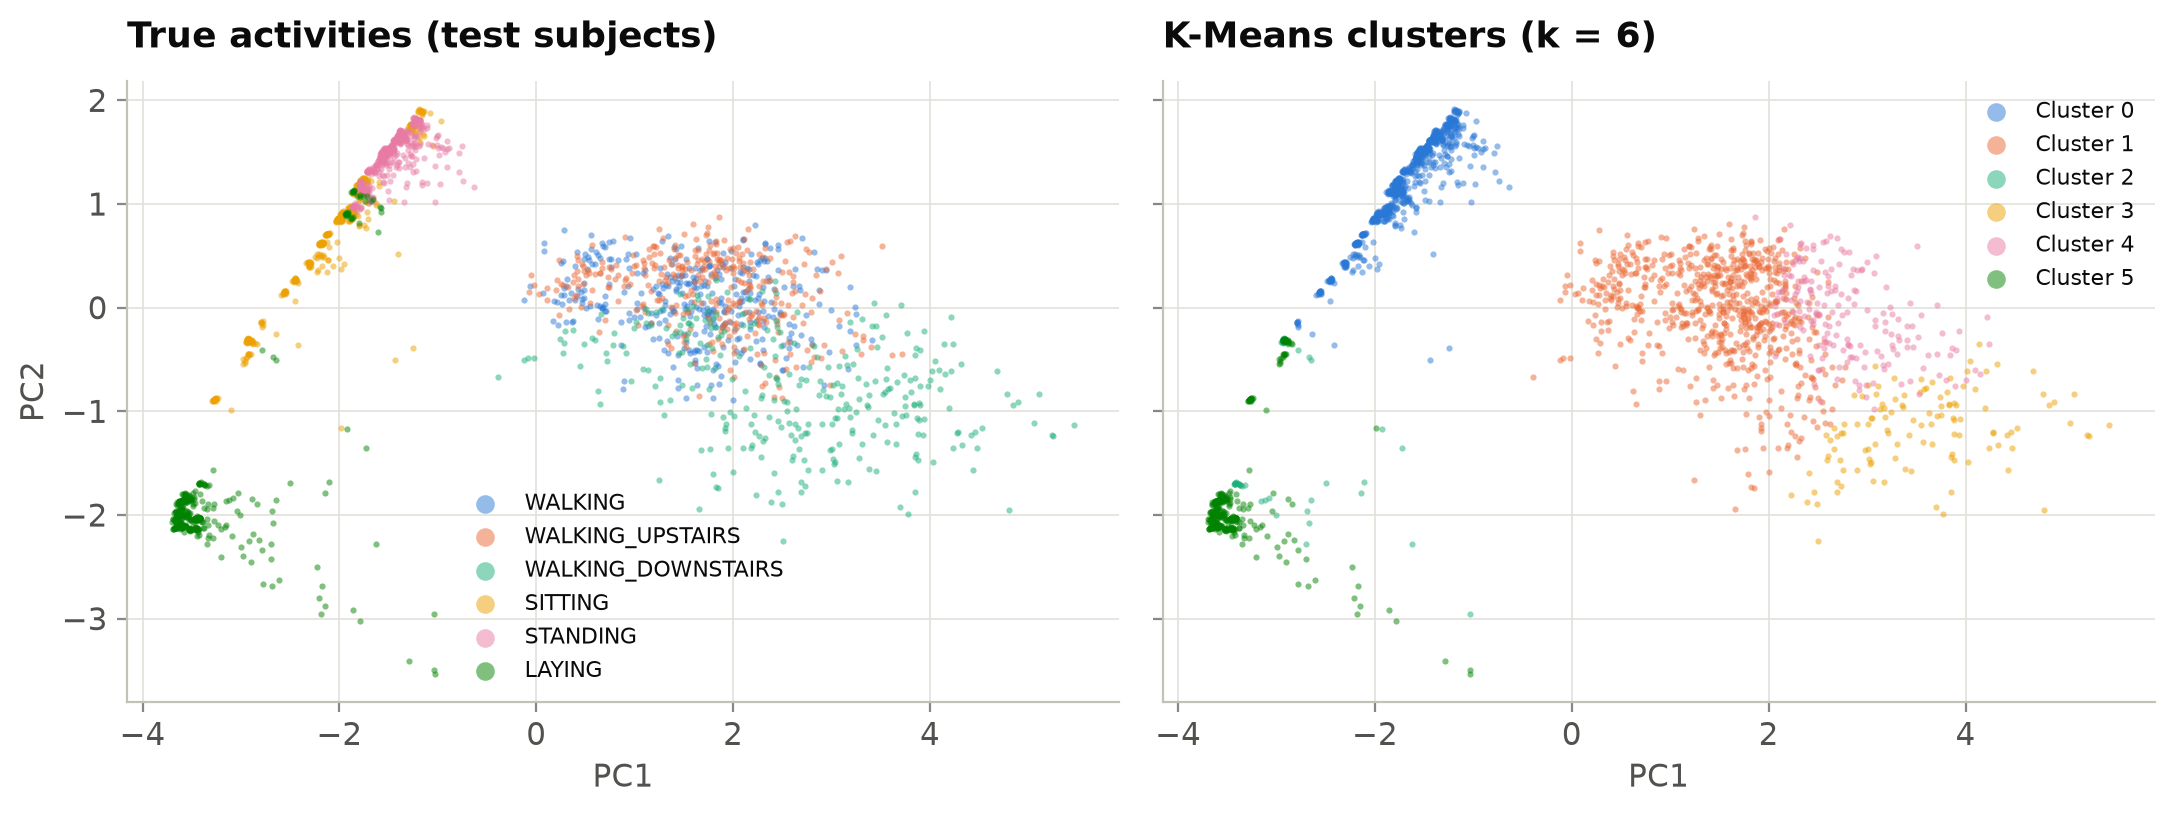
\includegraphics[width=0.92\linewidth]{har_pca_clusters.png}
\caption{Test windows in PCA space, coloured by true activity (left) and by K-Means cluster (right)}
\label{fig:harpca}
\end{figure}
\begin{table}[H]
\centering
\caption{Unit 3: clustering results on the six unseen test subjects}
\label{tab:unit3}
\begin{tabular}{@{}lcccc@{}}
\toprule
\textbf{Method} & \textbf{Accuracy} & \textbf{ARI} & \textbf{Silhouette} & \textbf{Avg segment (windows)} \\
\midrule
K-Means ($K=6$) & 0.570 & 0.464 & 0.412 & 7.8 \\
Gaussian Mixture ($K=6$) & 0.612 & 0.486 & 0.357 & 11.1 \\
True activity labels & 1.000 & 1.000 & 0.257 & 29.5 \\
\bottomrule
\end{tabular}
\end{table}
\textbf{Interpretation (Figure~\ref{fig:harpca}, Table~\ref{tab:unit3}).} Clustering recovers the coarse structure.
Laying forms its own tight cluster, and the dynamic activities form a separate cloud. GMM reaches 61.2\% accuracy and
K-Means 57.0\%; random guessing over six classes would give 16.7\%. K-Means merges Sitting and Standing into one cluster
and splits the walking cloud along boundaries that do not match Walking, Upstairs and Downstairs. Interestingly, the
clusters have a \emph{higher} silhouette than the true labels (0.41 vs 0.26): the geometric ``natural groups'' in feature
space are not the same as the semantic activities. Clustering also ignores time, so its labels flicker, with segments of
only 7.8–11.1 windows against 29.5 in reality.

\section{Unit 4 – Sequential Dataset Description}
Unit 4 uses the same UCI HAR recordings, treated as \textbf{time series}:
\begin{itemize}
\item \textbf{Sequence identifier:} the subject id. Each subject's windows form one continuous, time-ordered sequence
(30 sequences; the six test sequences contain 2,286 windows in total).
\item \textbf{Sampling:} 50 Hz raw signal; one observation per 2.56 s window, with a 1.28 s step.
\item \textbf{Hidden state:} the activity in each window ($S=6$ states). \textbf{Observation:} the 10 engineered
features (unsupervised HMM), or the dataset's 561 accelerometer and gyroscope features (supervised HMM).
\item \textbf{Data quality:} there are no missing windows. \textbf{Limitation:} the data was recorded in a laboratory
protocol with a fixed waist-worn phone position.
\end{itemize}

\section{Unit 4 – Sequential Preprocessing and EDA}
Temporal order is preserved throughout. Rows are sorted by subject with a \emph{stable} sort, so the original time order
within each subject is kept, and each subject is passed to the model as a separate sequence. States therefore never
carry over from one person to the next. Scalers are fitted on the training subjects only. The EDA in
Figure~\ref{fig:hareda} shows that activities persist for long bouts and that the signal changes at bout boundaries.
Both properties are exactly what a first-order Markov chain of hidden states with state-dependent emissions describes.

\section{Unit 4 – Mathematical Formulation}
An HMM $\lambda=(\boldsymbol\pi,\mathbf A,\mathbf B)$ over hidden states $s_t\in\{1,\dots,S\}$ and observations
$\mathbf x_t$ is defined by \cite{rabiner,murphy}:
\begin{equation}
\pi_i=P(s_1=i),\qquad a_{ij}=P(s_{t+1}=j\mid s_t=i),\qquad b_j(\mathbf x_t)=\mathcal N(\mathbf x_t\mid\boldsymbol\mu_j,\boldsymbol\Sigma_j).
\end{equation}
The Markov assumption is that $s_{t+1}$ depends only on $s_t$. The \textbf{forward} and \textbf{backward} recursions are
\begin{equation}
\alpha_t(j)=b_j(\mathbf x_t)\sum_{i}\alpha_{t-1}(i)\,a_{ij},\qquad
\beta_t(i)=\sum_{j}a_{ij}\,b_j(\mathbf x_{t+1})\,\beta_{t+1}(j),
\end{equation}
and their product gives the posterior state probability used for ``most likely state per window'' decoding:
\begin{equation}
\gamma_t(i)=P(s_t=i\mid\mathbf x_{1:T})=\frac{\alpha_t(i)\beta_t(i)}{\sum_j\alpha_t(j)\beta_t(j)} .
\end{equation}
\textbf{Viterbi} \cite{viterbi} finds the single most likely state sequence by dynamic programming, with back-pointers $\psi_t$:
\begin{equation}
\delta_t(j)=\max_i\big[\delta_{t-1}(i)+\log a_{ij}\big]+\log b_j(\mathbf x_t),\qquad
\psi_t(j)=\arg\max_i\big[\delta_{t-1}(i)+\log a_{ij}\big].
\end{equation}
\textbf{Unsupervised training} uses Baum–Welch (EM) \cite{baum}. It re-estimates, for example,
$a_{ij}=\sum_t\xi_t(i,j)/\sum_t\gamma_t(i)$, where $\xi_t(i,j)$ is the posterior probability of the transition
$i\to j$. \textbf{Supervised training} estimates the Markov chain by counting (maximum likelihood, +1 smoothing):
$a_{ij}=(n_{ij}+1)/\sum_k(n_{ik}+1)$. In the \textbf{hybrid HMM} the emission is a classifier's posterior divided by the
class prior, a scaled likelihood \cite{bourlard}: $b_j(\mathbf x)\propto P(s=j\mid\mathbf x)/P(s=j)$. All recursions are computed in log
space or with per-step scaling to avoid numerical underflow.

\section{Unit 4 Proposed System Architecture / Workflow}
\begin{figure}[H]
\centering
\begin{tikzpicture}[node distance=0.4cm and 0.45cm, font=\small,
  box/.style={draw=navy, fill=lightblue, rounded corners=3pt, minimum height=1.1cm, text width=2.2cm, align=center},
  hl/.style={box, fill=lightorange, draw=accent}, arr/.style={-{Stealth[length=2.5mm]}, thick, navy}]
\node[box] (a) {Per-subject ordered sequences};
\node[box, right=of a] (b) {Features: 10 (unsup.) / 561 (sup.)};
\node[hl, above right=0.15cm and 0.45cm of b] (c) {Baum–Welch EM (no labels)};
\node[hl, below right=0.15cm and 0.45cm of b] (d) {Count $\mathbf A,\boldsymbol\pi$ + classifier emissions};
\node[box, right=2.9cm of b] (e) {Forward–backward \& Viterbi (hand-coded)};
\node[box, right=of e] (f) {Decoded activity sequence};
\node[box, below=0.9cm of f] (g) {Accuracy, F1, ARI, segment length};
\draw[arr] (a)--(b); \draw[arr] (b)--(c); \draw[arr] (b)--(d); \draw[arr] (c)--(e); \draw[arr] (d)--(e);
\draw[arr] (e)--(f); \draw[arr] (f)--(g);
\end{tikzpicture}
\caption{Unit 4 sequential modelling workflow (unsupervised and supervised HMM)}
\label{fig:wf4}
\end{figure}
Each subject's windows form one ordered sequence. In the \emph{unsupervised} path, Baum–Welch learns
$(\boldsymbol\pi,\mathbf A,\mathbf B)$ from the 10 features without labels: 6 states, full-covariance Gaussian emissions,
8 random restarts. In the \emph{supervised} path, $\mathbf A$ and $\boldsymbol\pi$ are counted from labelled training
sequences, and the emissions come from either an LDA classifier (one Gaussian per activity) or a logistic-regression
classifier (hybrid HMM) on the 561 features. Both paths decode each test subject with our own forward–backward and
Viterbi implementations.

\section{Results and Performance Evaluation}
\textbf{Verification of the hand-coded algorithms.} On a test subject, our forward–backward posteriors match
\texttt{hmmlearn}'s \texttt{predict\_proba} to within $1.5\times10^{-10}$, and our Viterbi path is identical to
\texttt{hmmlearn.predict}.

\begin{figure}[H]
\centering
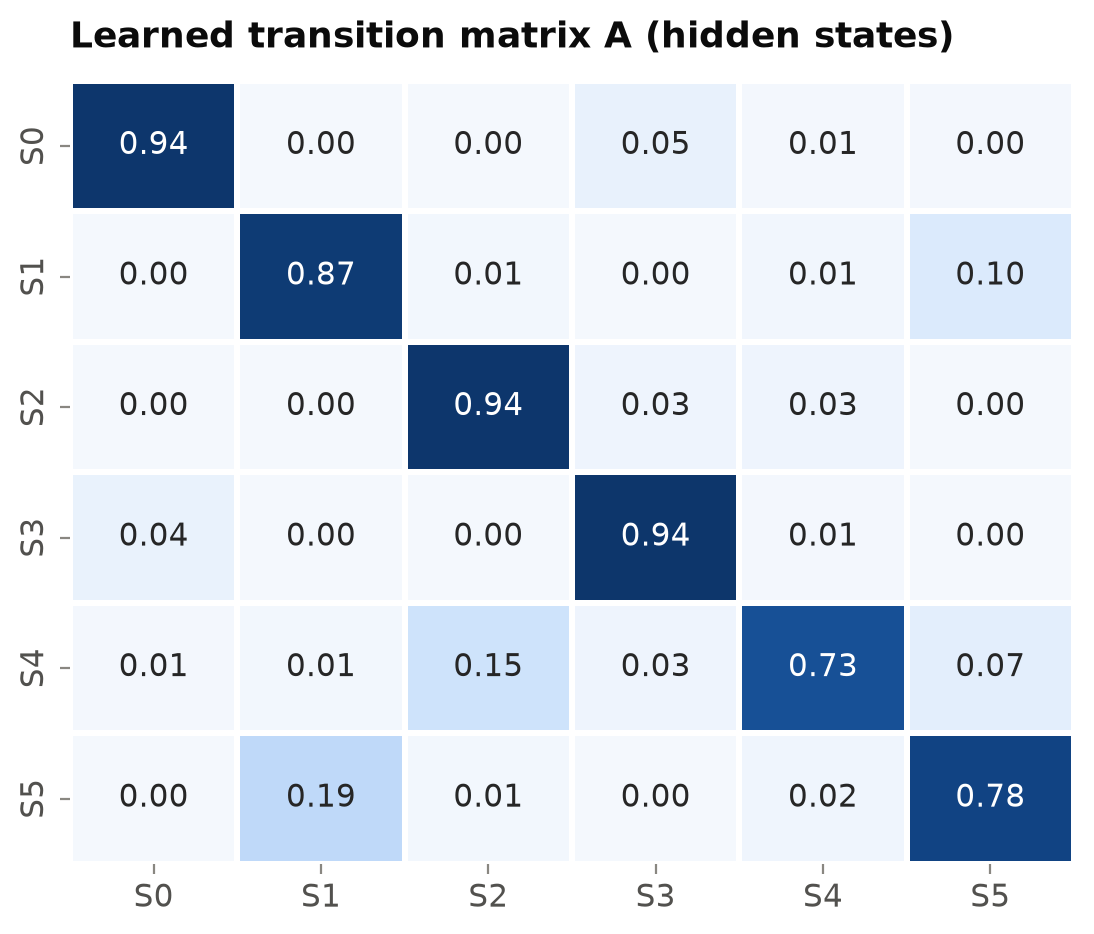
\includegraphics[width=0.40\linewidth]{har_transition_matrix.png}\hfill
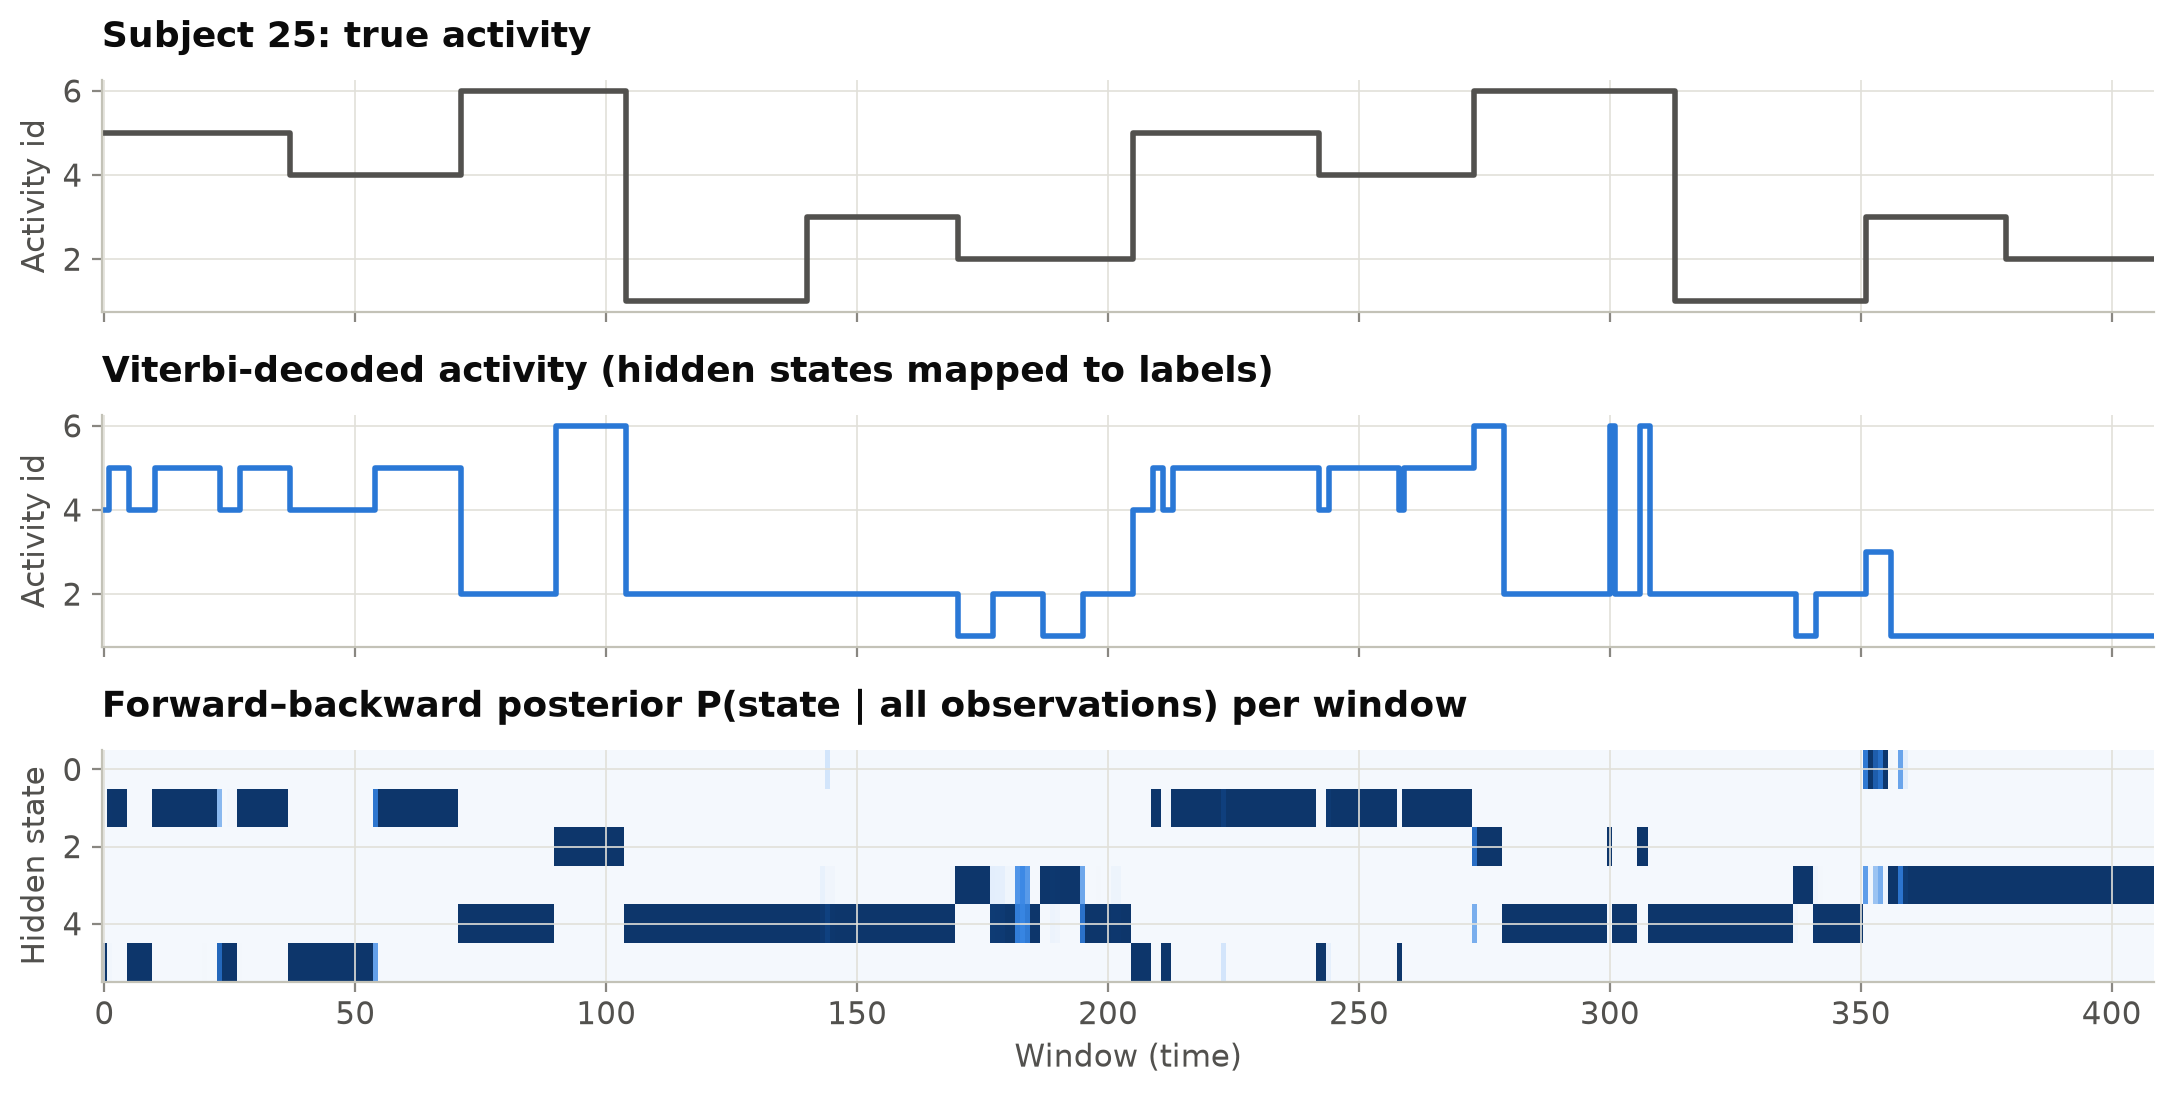
\includegraphics[width=0.58\linewidth]{har_decoded_timeline.png}
\caption{Unsupervised HMM: learned transition matrix (left); true vs Viterbi-decoded activities and forward–backward posteriors for test subject 25 (right)}
\label{fig:hmmunsup}
\end{figure}
\textbf{Interpretation (Figure~\ref{fig:hmmunsup}).} Without any labels, the HMM learns a strongly diagonal transition
matrix (0.73–0.94): states persist, as real activities do. The forward–backward posteriors are confident (near 0 or 1)
and switch exactly where the true activity changes, so the model detects \emph{when} transitions happen.

\begin{table}[H]
\centering
\caption{Unit 4: sequence decoding on the six unseen test subjects (2,286 windows)}
\label{tab:unit4}
\begin{tabular}{@{}llccc@{}}
\toprule
\textbf{Model} & \textbf{Decoding} & \textbf{Accuracy} & \textbf{Macro F1} & \textbf{Avg segment} \\
\midrule
Unsupervised Gaussian HMM (10 features) & Viterbi & 0.598 & – & 11.7 \\
LDA emissions (561 features) & per window, no HMM & 0.968 & 0.967 & 18.5 \\
LDA emissions + HMM & Viterbi & 0.975 & 0.974 & 25.6 \\
Logistic-regression emissions & per window, no HMM & 0.964 & 0.966 & 15.9 \\
\rowcolor{lightorange} Hybrid HMM (logistic regression) & Viterbi & \textbf{0.987} & \textbf{0.988} & 27.4 \\
Hybrid HMM (logistic regression) & forward–backward & 0.987 & 0.988 & 27.4 \\
\midrule
True activity sequence & – & 1.000 & 1.000 & 29.5 \\
\bottomrule
\end{tabular}
\end{table}
\begin{figure}[H]
\centering
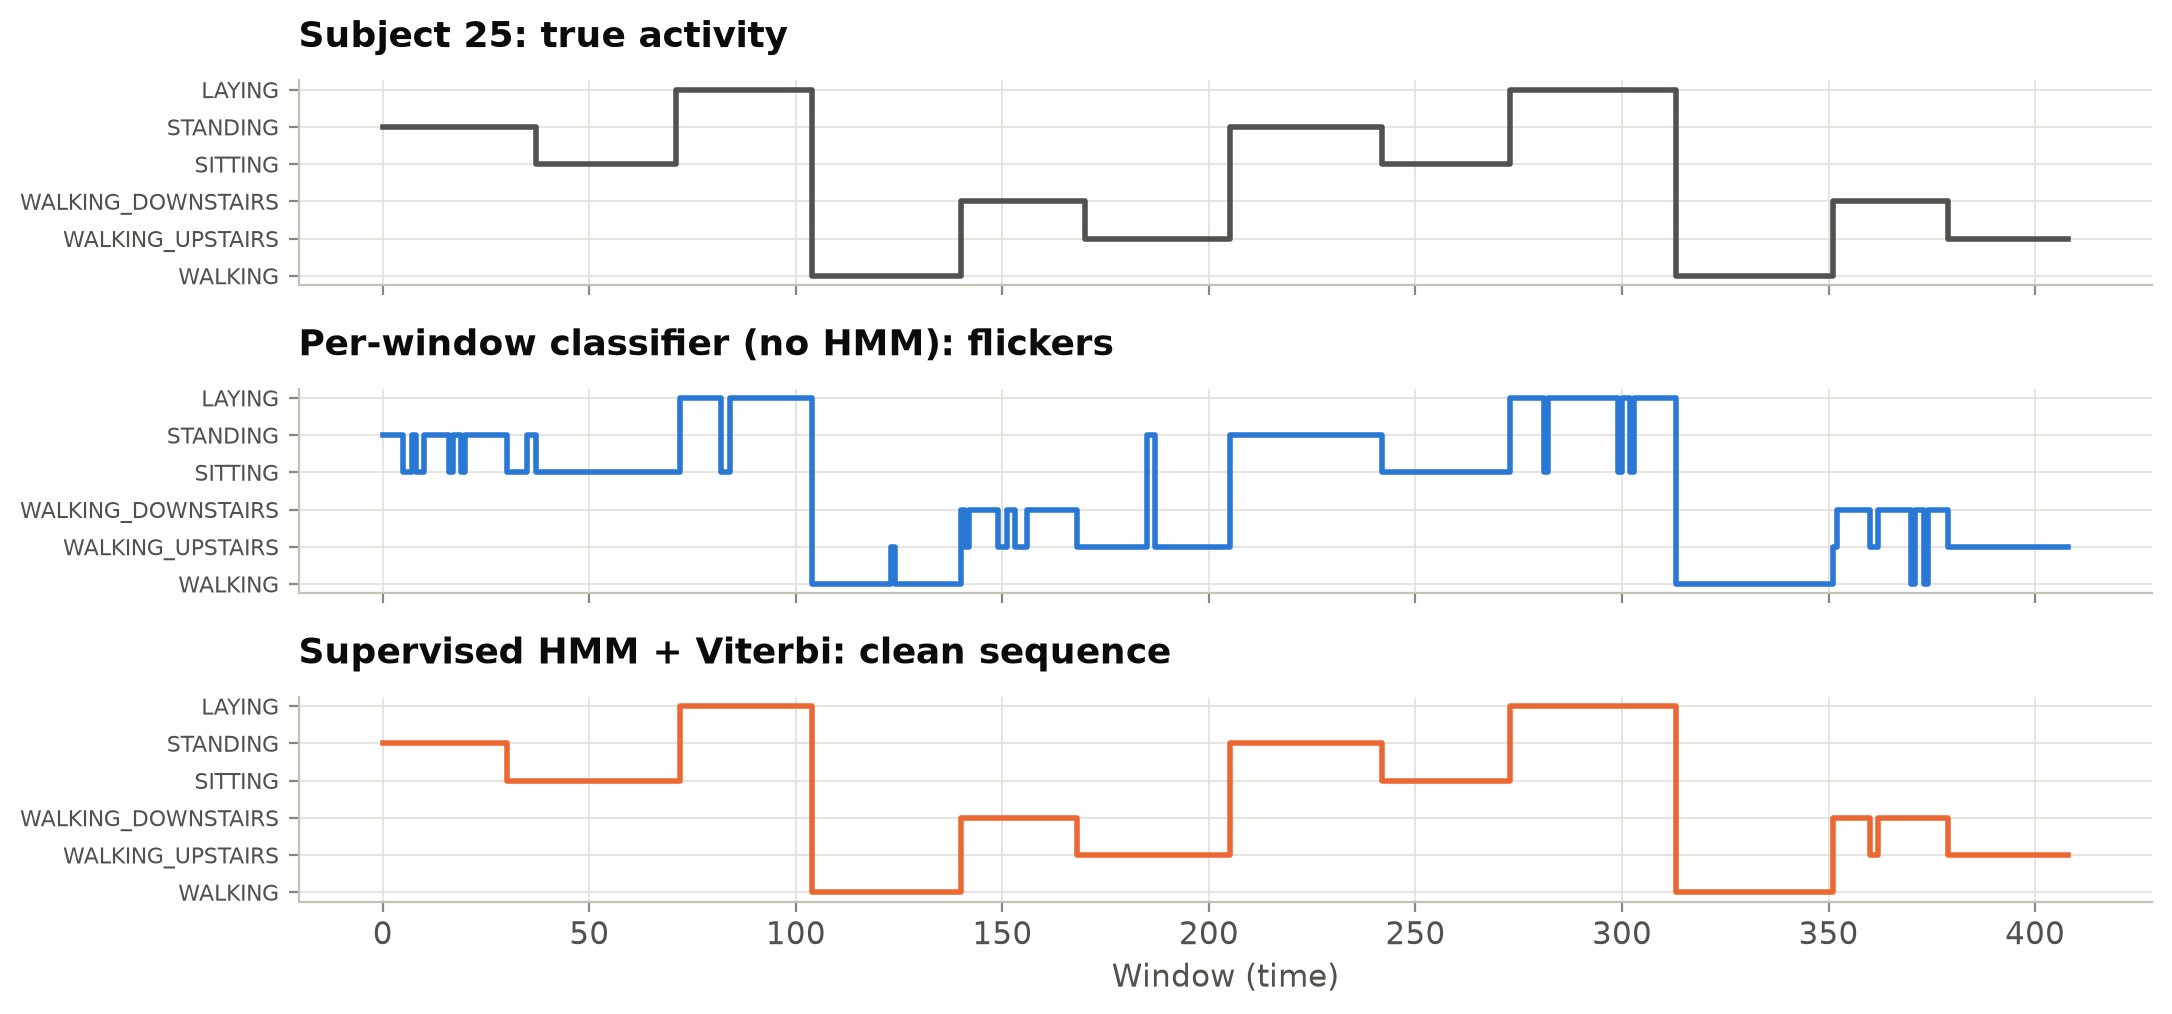
\includegraphics[width=0.56\linewidth]{har_supervised_timeline.png}\hfill
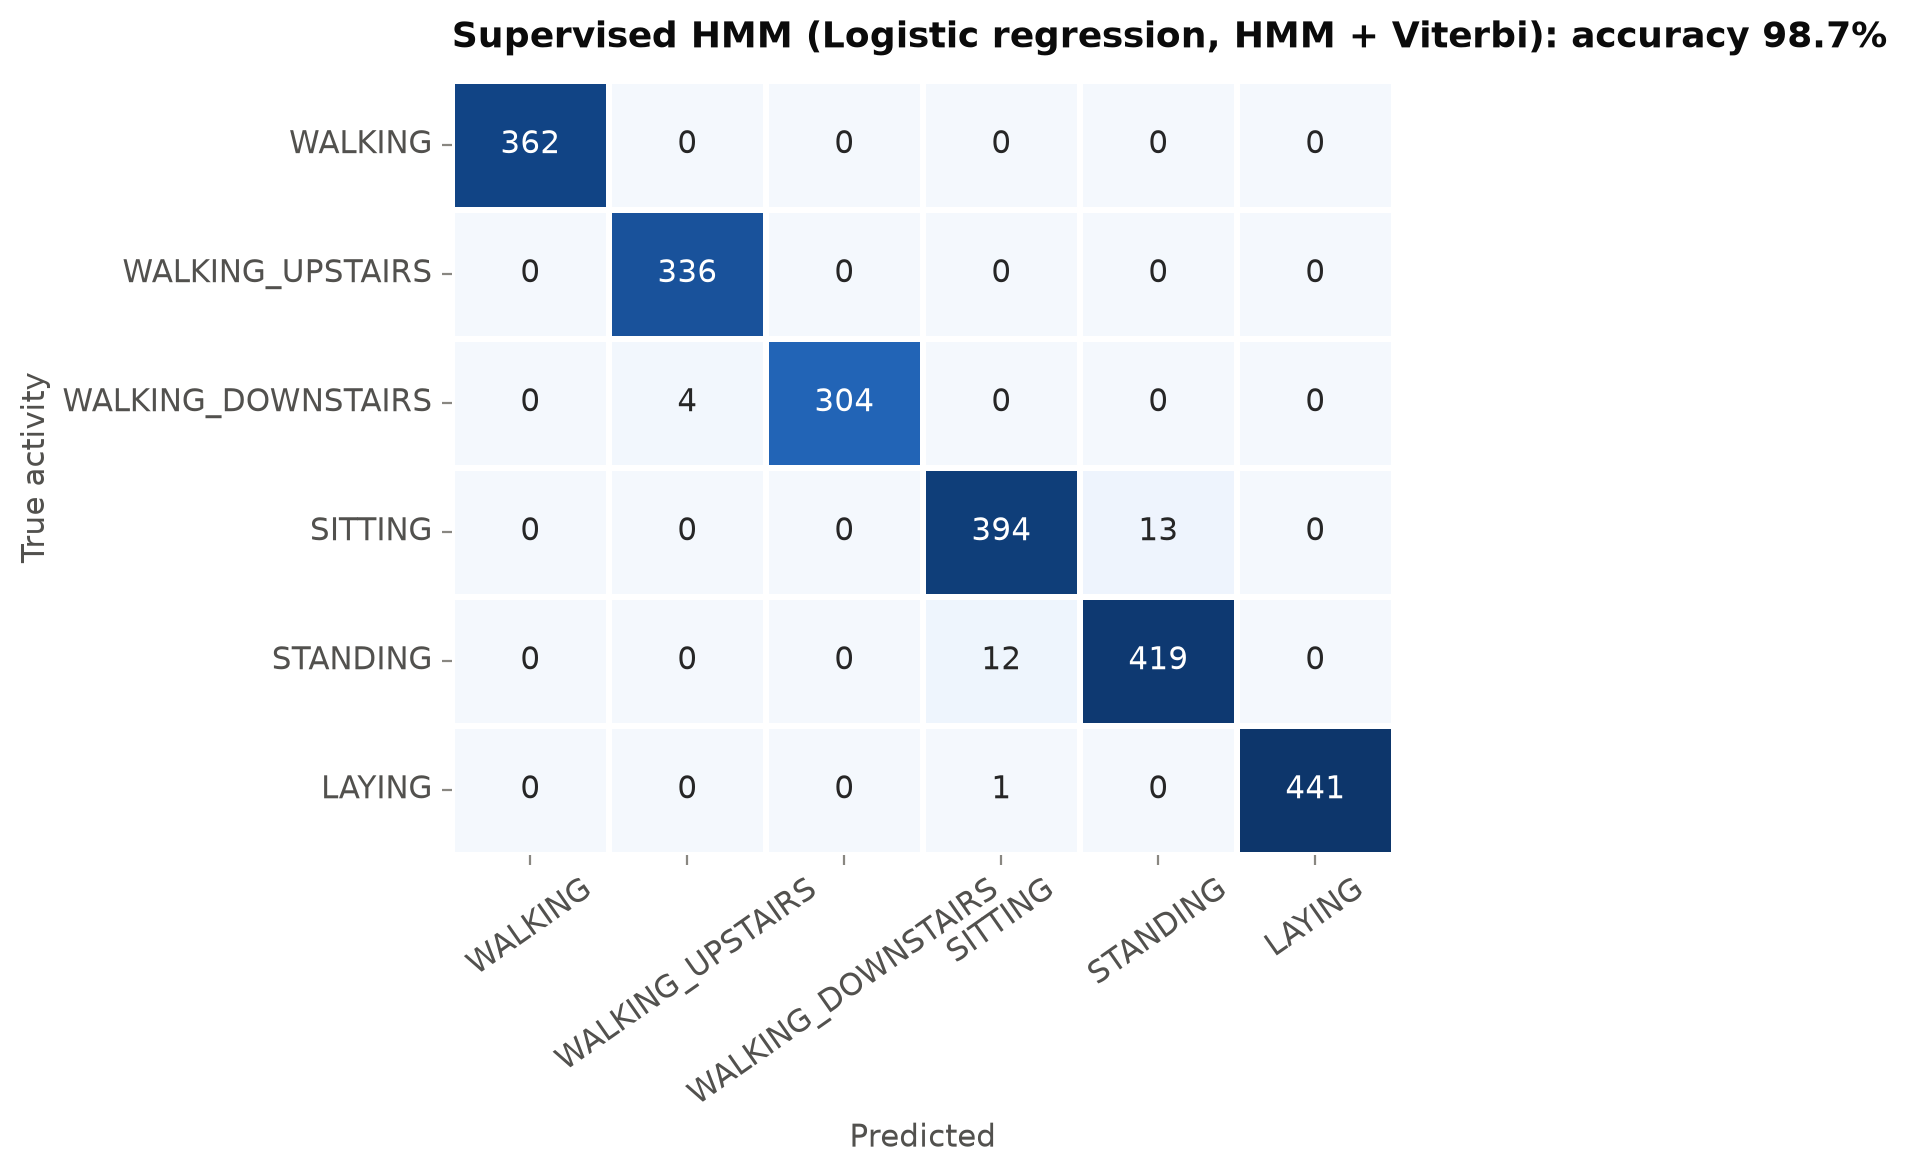
\includegraphics[width=0.42\linewidth]{har_confusion_supervised.png}
\caption{Supervised hybrid HMM: per-window classifier vs HMM + Viterbi for subject 25 (left); test confusion matrix (right)}
\label{fig:hmmsup}
\end{figure}
\textbf{Interpretation (Table~\ref{tab:unit4}, Figure~\ref{fig:hmmsup}).} The supervised hybrid HMM decodes the activities
of unseen people with \textbf{98.7\% accuracy} (macro F1 0.988). Holding the classifier fixed, adding the Markov chain
with Viterbi raises accuracy from 96.4\% to 98.7\%, removing \textbf{63\% of the errors}. It also lengthens the decoded
bouts from 15.9 to 27.4 windows, close to the true 29.5: Viterbi suppresses isolated one-window flickers that contradict
the surrounding activity. Walking and Walking Upstairs, the pair the unsupervised model confused most, are now classified
perfectly (362/362 and 336/336). Only 30 of 2,286 windows are wrong, and 25 of those are Sitting $\leftrightarrow$
Standing.

\section{Discussion, Findings and Limitations}
\begin{itemize}
\item \textbf{Clustering (Unit 3)} finds the geometric structure of the data but not the semantic activities. Similar
activities overlap in feature space, and time order is ignored.
\item \textbf{The unsupervised HMM} adds temporal consistency (segments of 11.7 vs 7.8 windows for K-Means) but no
accuracy gain (59.8\%). Its states must be discovered blindly from 10 accelerometer features, which cannot separate
stairs from walking or sitting from standing.
\item \textbf{The supervised HMM} shows the real value of sequential modelling. The Markov transition structure corrects
most of the remaining mistakes of a strong per-window classifier.
\item \textbf{State definitions and validation:} each state is defined as one activity. This is reasonable, but a
multi-state-per-activity or semi-Markov (explicit duration) model could represent within-activity dynamics better.
Validation is by unseen \emph{subjects}, the appropriate test of generalisation for sequential data.
\item \textbf{Limitations:} laboratory protocol, a fixed phone position, and only six test subjects.
\end{itemize}

\section{Chapter Conclusion}
Unit 3 showed that unsupervised clustering recovers the coarse static/dynamic structure of activity data (accuracy
57–61\%) but cannot label activities reliably. Unit 4 implemented and verified forward–backward and Viterbi, showed that
an unsupervised HMM learns realistic persistence without labels, and reached \textbf{98.7\% accuracy on unseen people}
with a supervised hybrid HMM. Its Markov chain removes 63\% of a per-window classifier's errors. These results are on a
different dataset from Units 1, 2 and 5, so they are not compared numerically with the other chapters.

\chapter{Advanced Predictive Modelling and Ensemble Learning (Unit 5)}

\section{Overview of Allotted Unit 5 Topics}
Group 10's PBL III topic is \textbf{Diabetes Prediction}: \emph{develop an intelligent diabetes prediction model using
patient health records, and investigate how effective different ensemble classifiers are at identifying individuals at
risk of diabetes.} The review requires at least three ensemble algorithms, a comparison against a baseline (Logistic
Regression or Decision Tree), and evaluation with F1-score and ROC-AUC.

\textbf{Ensemble learning} combines $M$ base learners $h_1,\dots,h_M$ into a stronger predictor
$H(\mathbf x)=\sum_m w_m h_m(\mathbf x)$. For averaged models, the error decomposes into bias and variance. Averaging
$M$ learners, each with variance $\sigma^2$ and pairwise correlation $\rho$, gives
\begin{equation}
\operatorname{Var}\!\Big[\tfrac{1}{M}\textstyle\sum_m h_m\Big]=\rho\,\sigma^2+\frac{1-\rho}{M}\,\sigma^2 ,
\label{eq:var}
\end{equation}
so \textbf{bagging} methods reduce variance by averaging many decorrelated trees, while \textbf{boosting} methods reduce
bias by adding learners sequentially, each correcting its predecessors' errors \cite{esl}. This chapter implements
\textbf{ten ensembles} from three families and compares them with two single-model baselines:
\begin{itemize}
\item \textbf{Bagging family:} Bagging \cite{breiman96}, Random Forest \cite{breiman01} and Extra Trees \cite{geurts}.
\item \textbf{Boosting family:} AdaBoost \cite{freund}, Gradient Boosting \cite{friedman}, XGBoost \cite{xgboost},
LightGBM \cite{lightgbm} and CatBoost \cite{catboost}.
\item \textbf{Meta-ensembles:} Soft Voting and Stacking \cite{wolpert} over the four strongest learners.
\item \textbf{Baselines:} Logistic Regression and a single Decision Tree (CART).
\end{itemize}

\section{Dataset Description and Preprocessing}
A new dataset is used for Unit 5: the \textbf{Diabetes Prediction Dataset} \cite{diabdata}. It contains
\dbRowsRaw{} electronic patient records with eight predictors and a binary target (diabetes yes/no).

\begin{table}[H]
\centering
\caption{Attributes of the Diabetes Prediction Dataset}
\label{tab:dbattr}
\renewcommand{\arraystretch}{1.2}
\begin{tabularx}{\linewidth}{@{}l l >{\raggedright\arraybackslash}X@{}}
\toprule
\textbf{Attribute} & \textbf{Type} & \textbf{Description / range} \\
\midrule
gender & categorical & Female, Male (and 18 records ``Other'') \\
age & continuous & 0.08–80 years \\
hypertension & binary & 1 if the patient has hypertension (7.5\%) \\
heart\_disease & binary & 1 if the patient has heart disease (3.9\%) \\
smoking\_history & categorical & never, former, current, not current, ever, No Info \\
bmi & continuous & body-mass index, 10.0–95.7 kg/m$^2$ \\
HbA1c\_level & continuous & glycated haemoglobin, 3.5–9.0\% (average blood sugar over 2–3 months) \\
blood\_glucose\_level & continuous & blood glucose at the time of measurement, 80–300 mg/dL \\
\midrule
\textbf{diabetes} & \textbf{binary target} & 1 = diabetic (8.5\% before cleaning) \\
\bottomrule
\end{tabularx}
\end{table}

\textbf{Relevance.} These are exactly the routinely collected variables a clinician sees: demographics, comorbidities,
lifestyle, and the two laboratory markers used for diagnosis \cite{ada}. The dataset is large enough
(\dbRowsRaw{} records) for a reliable comparison of many ensembles with cross-validation.

\textbf{Preprocessing.}
\begin{enumerate}
\item \textbf{Duplicates:} \dbDup{} exact duplicate records were removed. Otherwise identical rows could appear in both
the training and test sets and inflate the scores.
\item \textbf{Rare category:} gender ``Other'' (18 records) was dropped, since it is too rare to learn from. This leaves
\textbf{\dbRowsClean{} patients}, with a diabetes prevalence of \dbPrev.
\item \textbf{Missing information:} there are no null values, but smoking history is ``No Info'' for about 36\% of
patients. This is kept as its own category, because whether smoking was recorded is itself informative, and imputing
it would invent information.
\item \textbf{Outliers:} all values are clinically plausible, so none were removed; high values are genuine high-risk
patients.
\item \textbf{Encoding and scaling:} one-hot encoding for gender and smoking history, and standardisation of numeric
features, inside a scikit-learn \texttt{Pipeline}. Standardisation is needed by Logistic Regression and harmless for
trees.
\item \textbf{Split:} a stratified 80/20 split into \dbTrain{} training and \dbTest{} test patients, keeping the
prevalence in both sets. The test set is used once. All model comparisons use \textbf{5-fold stratified
cross-validation} on the training set.
\end{enumerate}
\begin{pycode}
df = df_raw.drop_duplicates()
df = df[df.gender != "Other"].reset_index(drop=True)
pre = ColumnTransformer([("num", StandardScaler(), ["age", "bmi", "HbA1c_level", "blood_glucose_level",
                                                    "hypertension", "heart_disease"]),
                         ("cat", OneHotEncoder(handle_unknown="ignore"), ["gender", "smoking_history"])])
X_train, X_test, y_train, y_test = train_test_split(X, y, test_size=0.2, stratify=y, random_state=42)
cv = StratifiedKFold(n_splits=5, shuffle=True, random_state=42)
\end{pycode}

\section{EDA and Feature Analysis}
\begin{figure}[H]
\centering
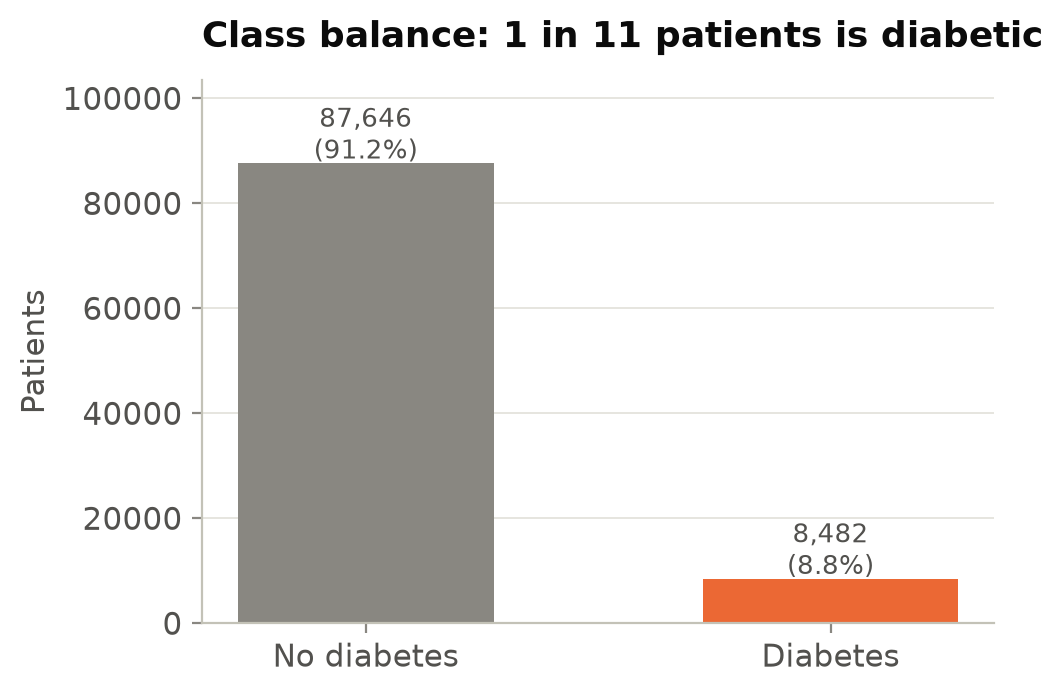
\includegraphics[width=0.40\linewidth]{db_class_balance.png}\hfill
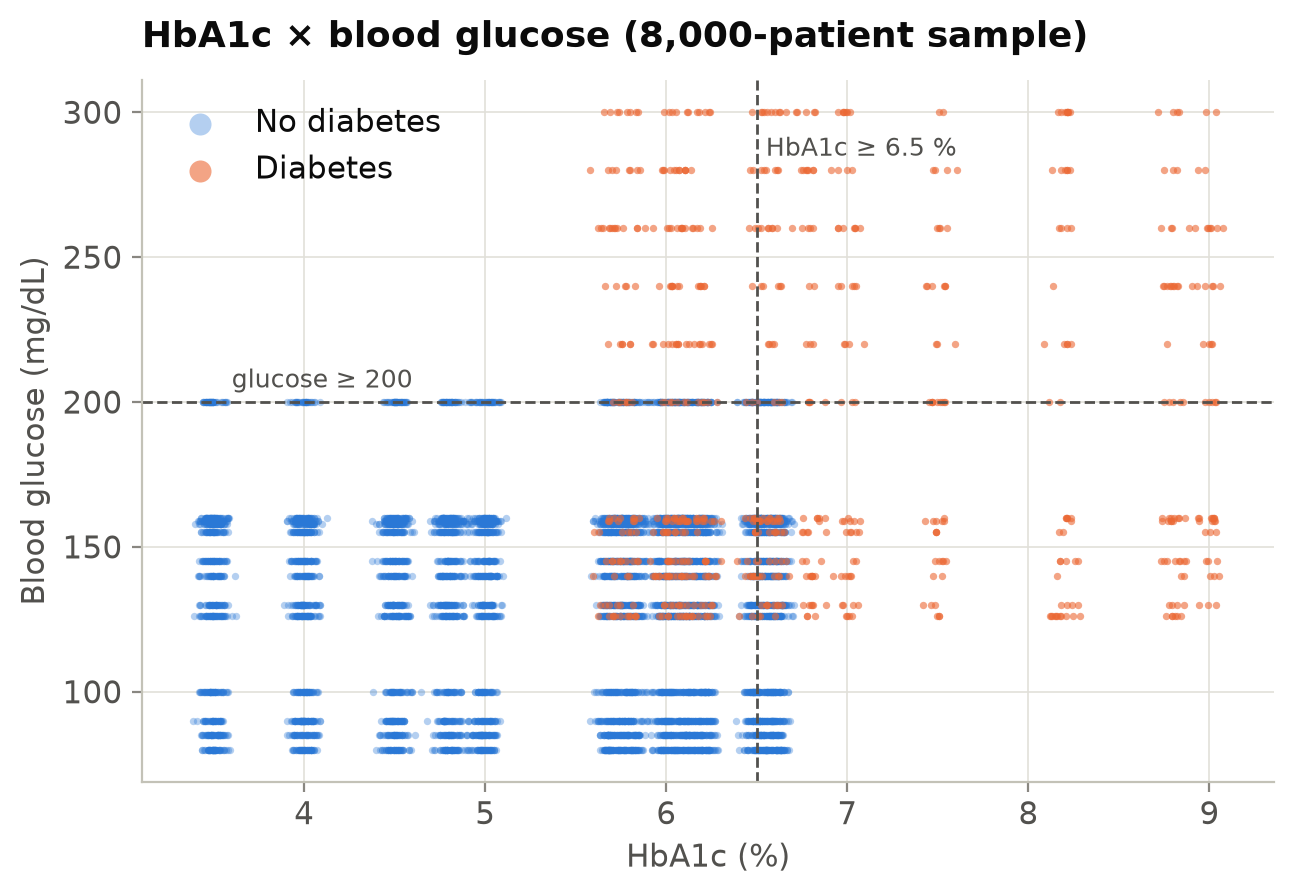
\includegraphics[width=0.56\linewidth]{db_hba1c_glucose.png}
\caption{Class balance (left) and HbA1c against blood glucose for 8,000 patients (right)}
\label{fig:dbbal}
\end{figure}
\textbf{Interpretation (Figure~\ref{fig:dbbal}).} Only \dbPrev{} of patients are diabetic, so the target is imbalanced. A
model that always predicts ``no diabetes'' would be 91\% accurate yet useless. We therefore judge models by
\textbf{F1-score, ROC-AUC and PR-AUC}, not accuracy. HbA1c and glucose are recorded at a small set of discrete levels.
Every patient with HbA1c $>$ 6.6\% or glucose $>$ 200 mg/dL is diabetic. These patients make up \dbRuleShare{} of the
data and account for \dbRuleCapture{} (two-thirds) of all diabetics; they are easy to classify. The remaining third of
diabetics have laboratory values inside the normal range, and these \emph{hard cases} are where a model must combine
age, BMI, comorbidities and the laboratory values.

\begin{figure}[H]
\centering
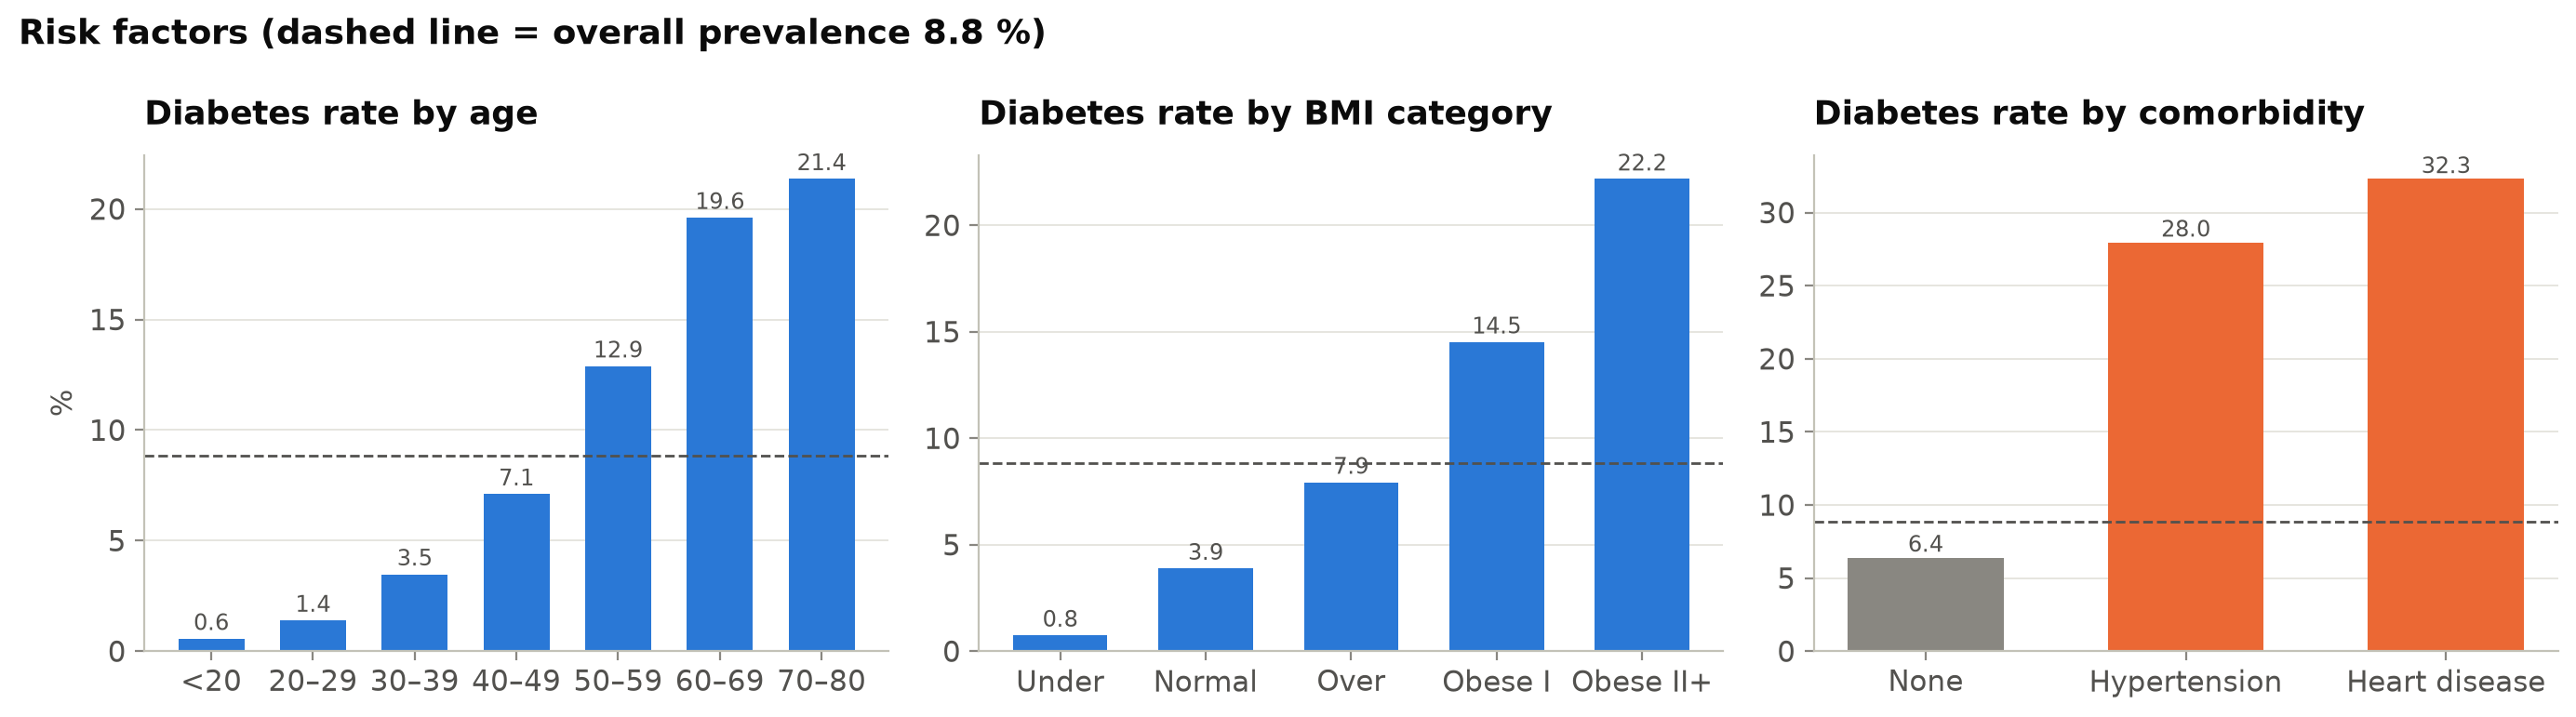
\includegraphics[width=\linewidth]{db_risk_factors.png}
\caption{Diabetes rate by age group, BMI category and comorbidity (dashed line = overall prevalence)}
\label{fig:dbrisk}
\end{figure}
\textbf{Interpretation (Figure~\ref{fig:dbrisk}).} Risk rises steeply and non-linearly with age, from 0.6\% under 20
to 21.4\% at 70–80. It also rises with BMI, from 3.9\% at normal weight to 22.2\% in severe obesity, and with
comorbidity: 28.0\% with hypertension and 32.3\% with heart disease, against 6.4\% without either. These monotone but
non-linear, interacting effects are what tree ensembles capture without manual feature engineering.

\begin{figure}[H]
\centering
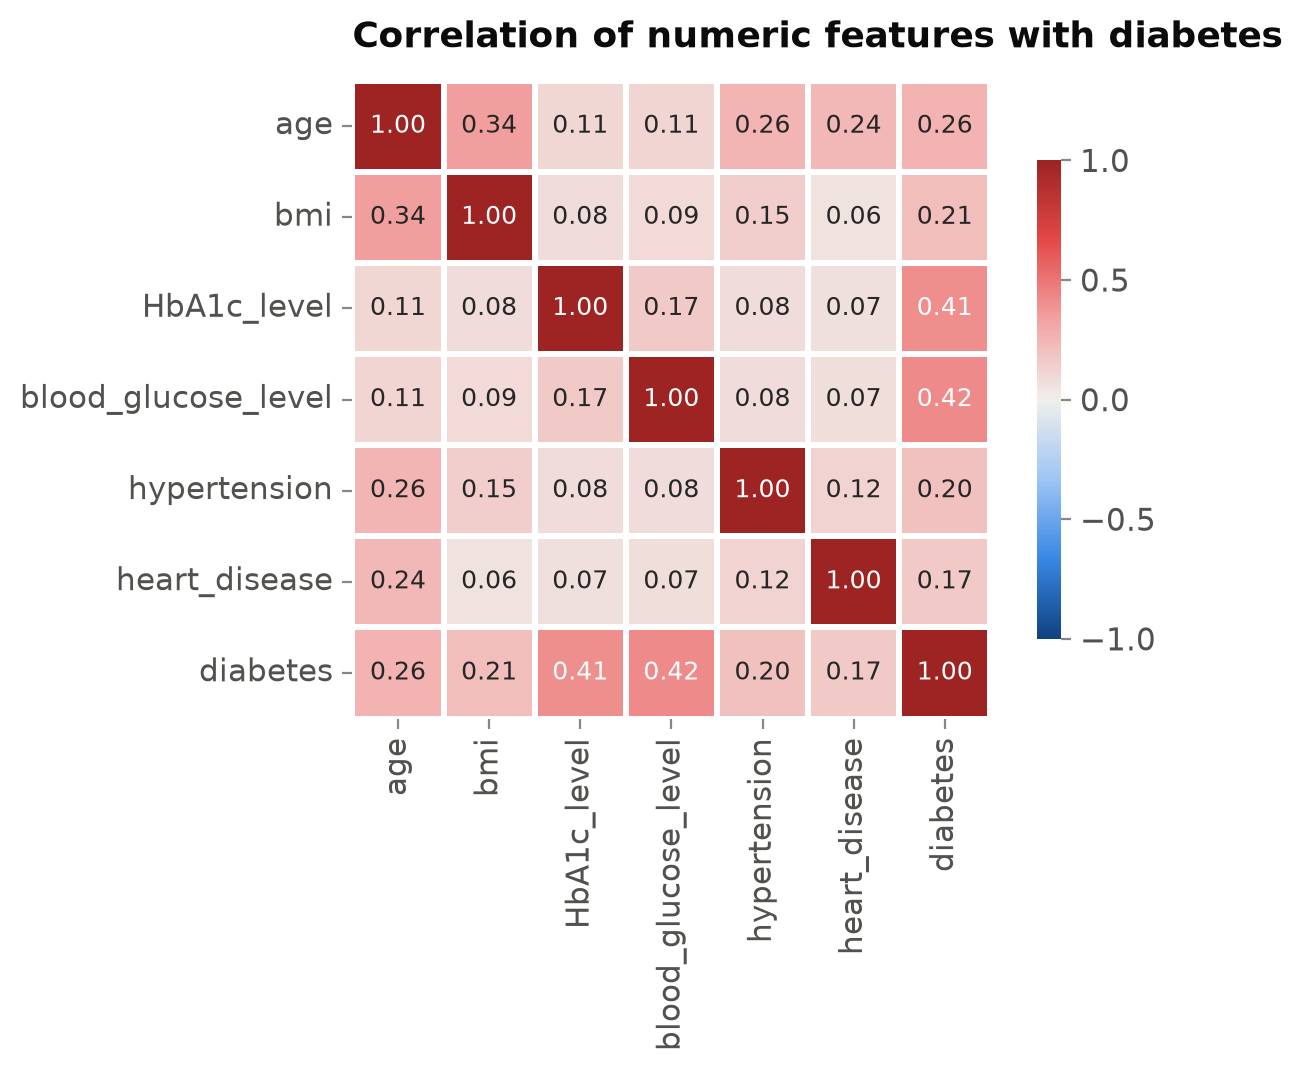
\includegraphics[width=0.49\linewidth]{db_correlation.png}\hfill
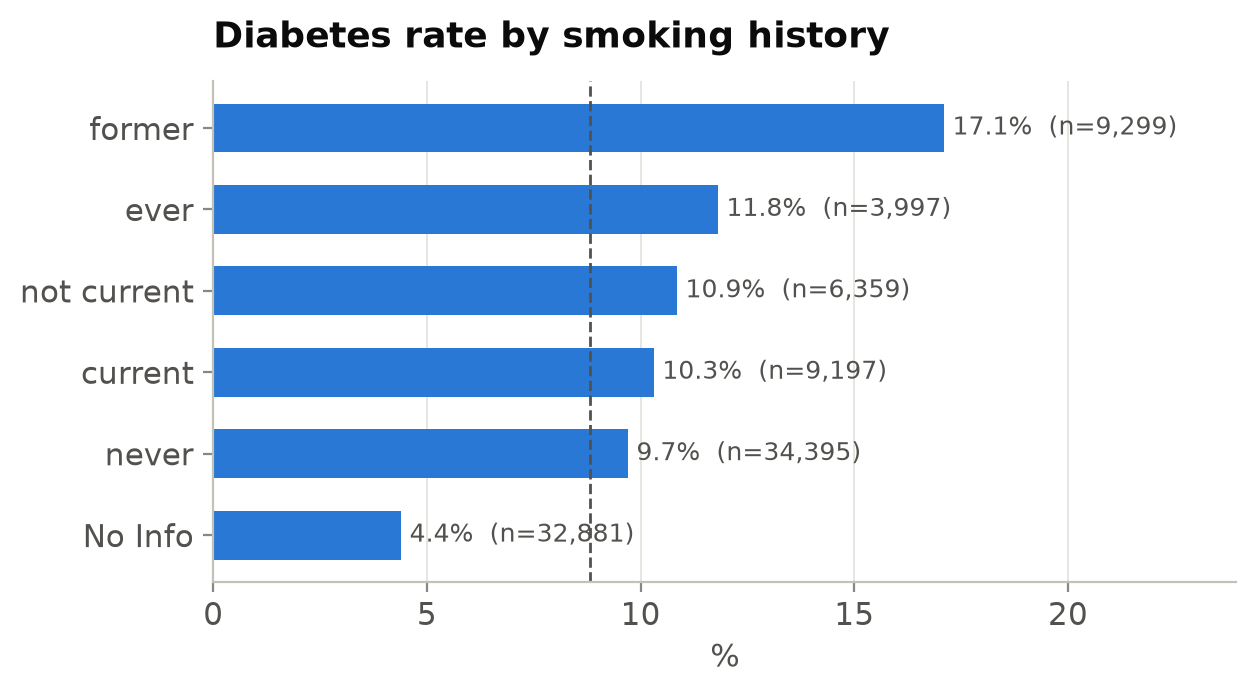
\includegraphics[width=0.49\linewidth]{db_smoking.png}
\caption{Correlation of numeric features with diabetes (left); diabetes rate by smoking history (right)}
\label{fig:dbcorr}
\end{figure}
\textbf{Interpretation (Figure~\ref{fig:dbcorr}).} Blood glucose (0.42) and HbA1c (0.41) are the strongest single
correlates, followed by age (0.26), BMI (0.21), hypertension (0.20) and heart disease (0.17). Correlations among the
predictors are weak (all $\le$0.34), so multicollinearity is not a concern. Former smokers have the highest rate
(17.1\%). Patients with ``No Info'' have the lowest (4.4\%), largely because this group contains many children, which
confirms that the missingness is informative and should be kept as a category.

\begin{figure}[H]
\centering
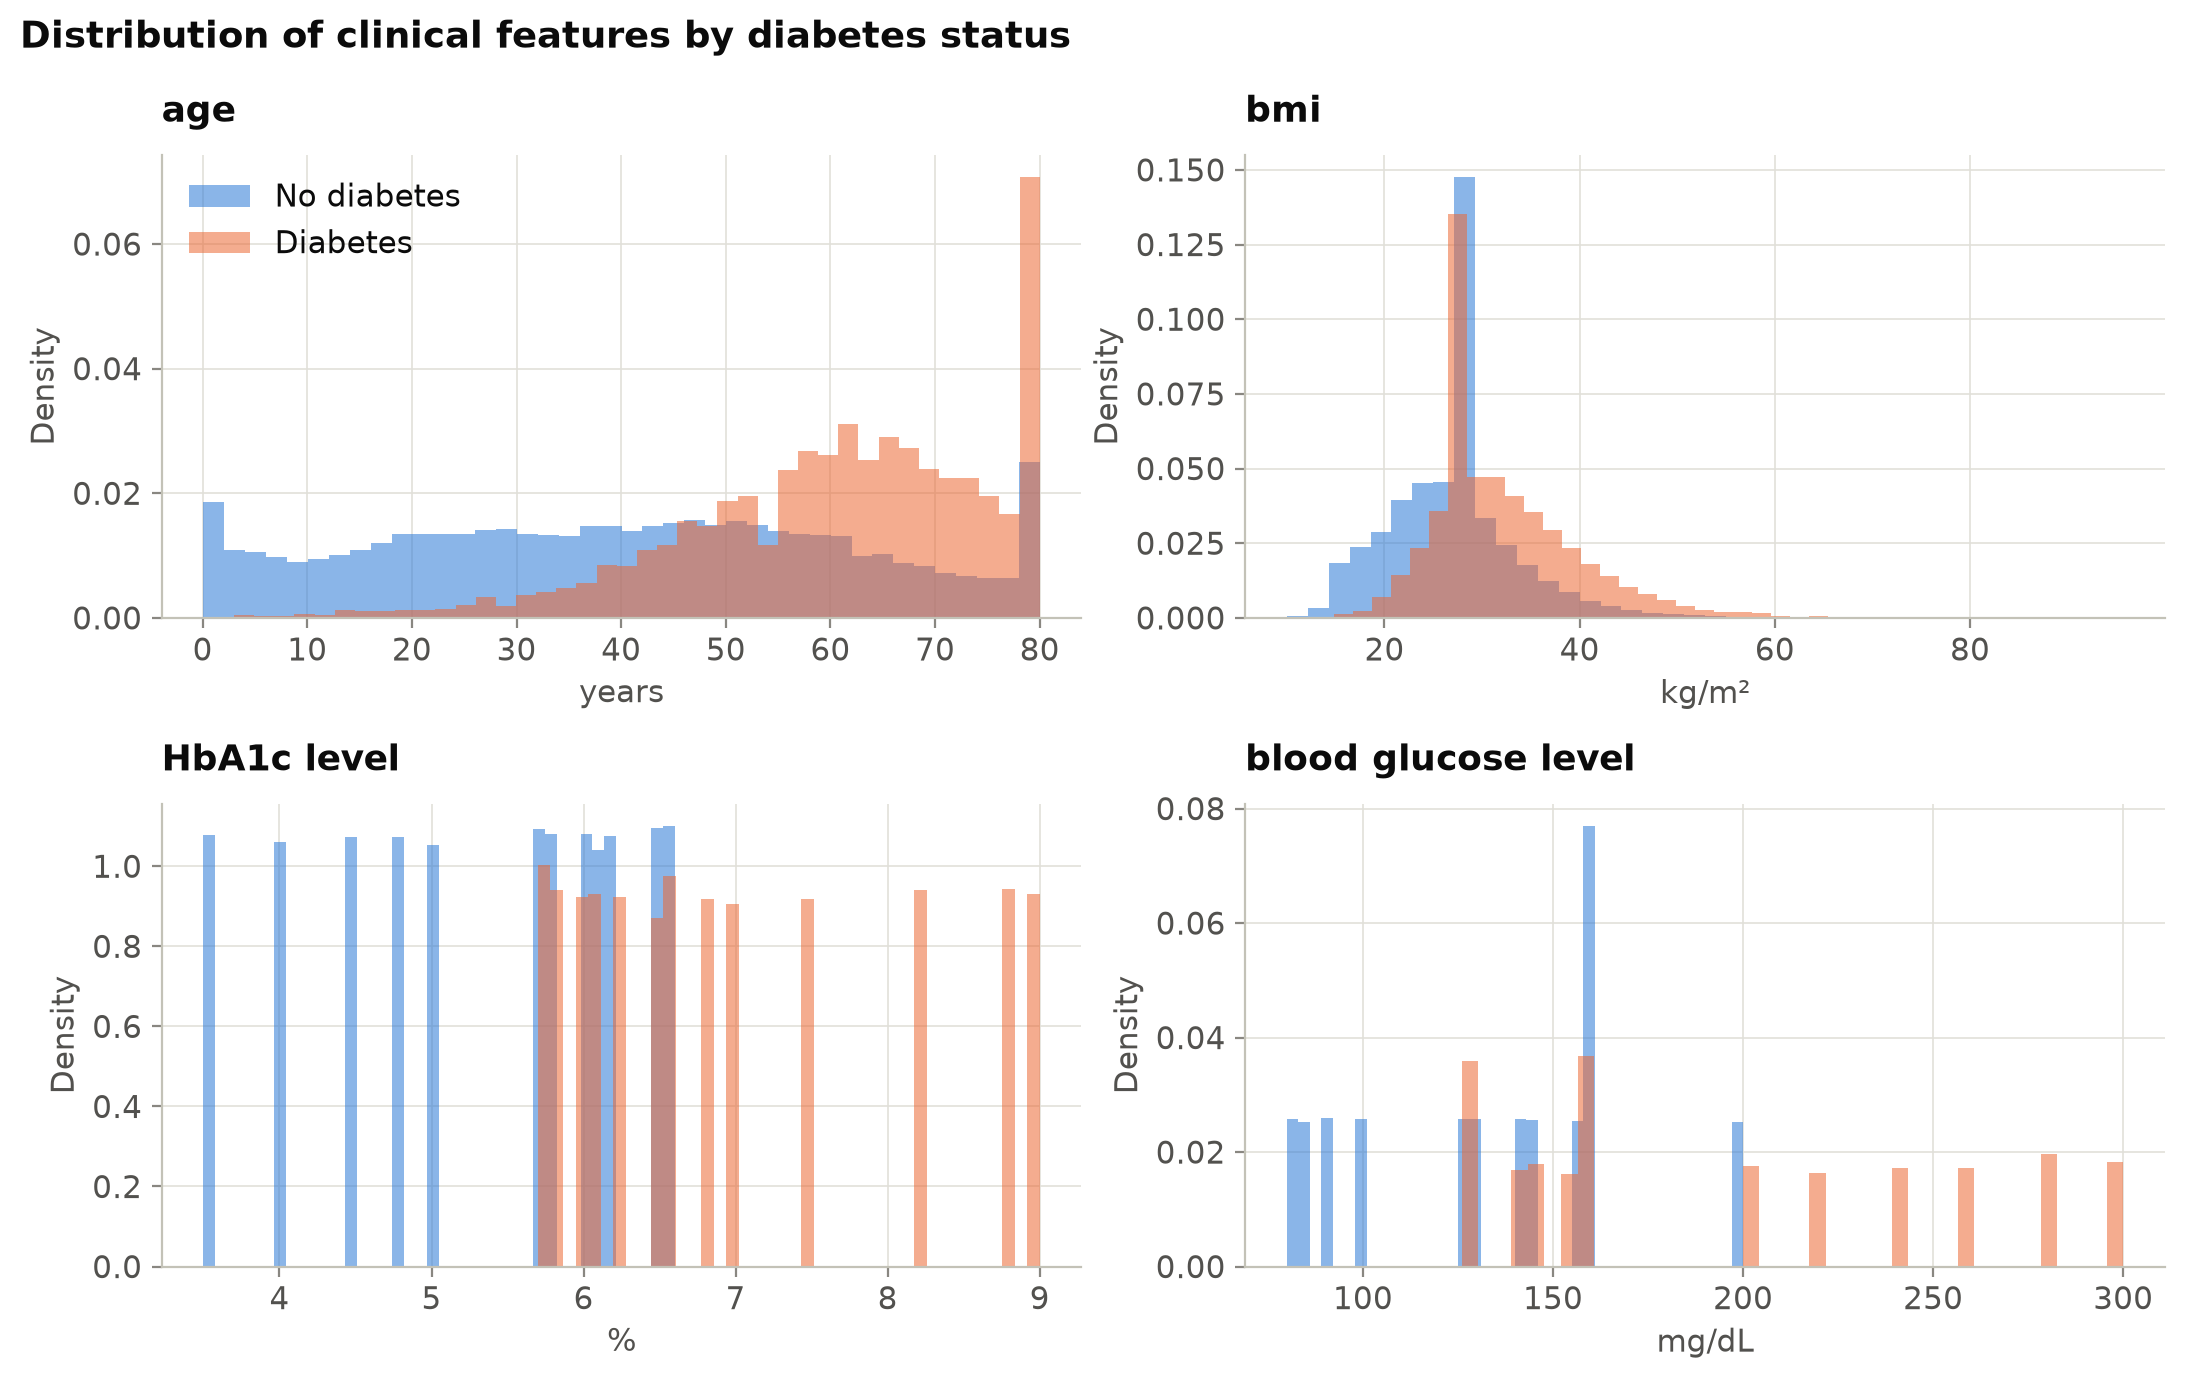
\includegraphics[width=\linewidth]{db_feature_distributions.png}
\caption{Distribution of the four clinical features by diabetes status}
\label{fig:dbdist}
\end{figure}
\textbf{Interpretation (Figure~\ref{fig:dbdist}).} Diabetic patients are older and have higher BMI. Their HbA1c and
glucose distributions extend into ranges (HbA1c 6.8–9\%, glucose 220–300) that never occur in non-diabetics, while
overlapping substantially with non-diabetics at lower levels.

\section{Proposed Workflow / Architecture}
\begin{figure}[H]
\centering
\resizebox{\linewidth}{!}{%
\begin{tikzpicture}[font=\small,
  box/.style={draw=navy, fill=lightblue, rounded corners=3pt, minimum height=1.35cm, text width=3.0cm, align=center},
  hl/.style={box, fill=lightorange, draw=accent}, gr/.style={box, fill=green!8, draw=green!50!black},
  arr/.style={-{Stealth[length=2.5mm]}, thick, navy}, bus/.style={thick, navy}]
\node[box] (a) at (0,0) {Patient records (100,000)};
\node[box] (b) at (3.8,0) {Clean: duplicates, rare category};
\node[box] (c) at (7.6,0) {Stratified 80/20 split};
\node[box] (d) at (11.4,0) {Pipeline: one-hot + scaling};
\node[gr] (e) at (0,-2.6) {Baselines: Logistic Regression, Decision Tree};
\node[hl] (f) at (3.8,-2.6) {Bagging: Bagging, Random Forest, Extra Trees};
\node[hl] (g) at (7.6,-2.6) {Boosting: AdaBoost, GB, XGBoost, LightGBM, CatBoost};
\node[hl] (h) at (11.4,-2.6) {Meta-ensembles: Soft Voting, Stacking};
\node[box] (i) at (0,-5.2) {5-fold stratified CV (F1, ROC-AUC, PR-AUC)};
\node[box] (j) at (3.8,-5.2) {Final model = best CV F1};
\node[box] (k) at (7.6,-5.2) {LightGBM tuning; F1-optimal threshold (OOF)};
\node[box] (l) at (11.4,-5.2) {Test set: metrics, McNemar, SHAP};
\draw[arr] (a)--(b); \draw[arr] (b)--(c); \draw[arr] (c)--(d);
\coordinate (t1) at (0,-1.3); \coordinate (t2) at (0,-3.9);
\draw[bus] (d.south) -- (d.south |- t1);
\draw[bus] (e.north |- t1) -- (h.north |- t1);
\foreach \n in {e,f,g,h} \draw[arr] (\n.north |- t1) -- (\n.north);
\foreach \n in {e,f,g,h} \draw[bus] (\n.south) -- (\n.south |- t2);
\draw[bus] (e.south |- t2) -- (h.south |- t2);
\draw[arr] (e.south |- t2) -- (i.north);
\draw[arr] (i)--(j); \draw[arr] (j)--(k); \draw[arr] (k)--(l);
\end{tikzpicture}}
\caption{Unit 5 workflow: preprocessing, 2 baselines and 10 ensembles, CV-based selection, tuning, threshold optimisation and test evaluation}
\label{fig:wf5}
\end{figure}
\textbf{Stages.} (1) The patient records are cleaned and split (stratified) before any fitting. (2) Every model is a
pipeline of the same preprocessing plus the classifier, so encoding and scaling never see validation or test data.
(3) The twelve models are compared with identical 5-fold stratified CV. (4) The final model is the one with the highest CV F1, chosen without
looking at the test set; LightGBM is additionally tuned by randomised search. (5) Because the classes are imbalanced, the decision threshold is chosen to maximise F1 on
\emph{out-of-fold} training predictions. (6) The held-out test set is used once, for the final metrics, McNemar's
significance test and SHAP interpretation.

\section{Algorithm Theory and Mathematical Formulation}
\subsection{Baselines}
\textbf{Logistic Regression} models $P(y=1\mid\mathbf x)=\sigma(\mathbf w^\top\mathbf x+b)$ and minimises the log-loss
(Chapter 2). It is linear in the features, so it cannot represent the steep, interacting thresholds seen in the EDA.
A \textbf{Decision Tree (CART)} recursively chooses the split that maximises the decrease in Gini impurity
$G=1-\sum_k p_k^2$. A fully grown tree has low bias but very high variance.

\subsection{Bagging family}
\textbf{Bagging} trains $M$ trees on bootstrap samples (drawn with replacement) and averages their predicted
probabilities, $\hat p(\mathbf x)=\frac1M\sum_m h_m(\mathbf x)$. By Equation~(\ref{eq:var}), averaging reduces variance
as long as the trees are not perfectly correlated. \textbf{Random Forest} decorrelates the trees further by considering
only a random subset of features ($\sqrt d$) at each split, which lowers $\rho$. \textbf{Extra Trees} also draws the
split thresholds at random, trading a little bias for further variance reduction.
\emph{Settings:} 200 bagged trees; 300 trees with \texttt{min\_samples\_leaf}=2 for RF and Extra Trees.

\subsection{Boosting family}
\textbf{AdaBoost} fits weak learners (decision stumps) sequentially. After round $m$, with weighted error
$\varepsilon_m$, the learner receives weight $\alpha_m=\tfrac12\ln\frac{1-\varepsilon_m}{\varepsilon_m}$, and the
misclassified samples are up-weighted, $w_i\leftarrow w_i\,e^{\alpha_m\,\mathbb 1[h_m(\mathbf x_i)\ne y_i]}$.
The final model is $H(\mathbf x)=\operatorname{sign}\sum_m\alpha_m h_m(\mathbf x)$.
\emph{Settings:} 300 estimators, learning rate 0.5.

\textbf{Gradient Boosting} builds an additive model $F_m(\mathbf x)=F_{m-1}(\mathbf x)+\eta\,h_m(\mathbf x)$, where each
tree $h_m$ is fitted to the negative gradient of the log-loss, the pseudo-residuals $r_{im}=y_i-p_{m-1}(\mathbf x_i)$.
\emph{Settings:} 300 trees of depth 3, learning rate $\eta=0.1$.

\textbf{XGBoost} minimises a regularised second-order approximation of the loss. For a tree with leaf weights $w_j$ and
gradient/Hessian sums $G_j,H_j$, the optimal leaf weight and the gain of a split are
\begin{equation}
w_j^\star=-\frac{G_j}{H_j+\lambda},\qquad
\text{Gain}=\tfrac12\Big[\frac{G_L^2}{H_L+\lambda}+\frac{G_R^2}{H_R+\lambda}-\frac{(G_L+G_R)^2}{H_L+H_R+\lambda}\Big]-\gamma .
\end{equation}
\textbf{LightGBM} uses the same objective with histogram-based split finding and \emph{leaf-wise} tree growth, which is
much faster. \textbf{CatBoost} uses \emph{ordered boosting} and symmetric (oblivious) trees, which reduces prediction
shift and over-fitting. \emph{Settings:} XGBoost and LightGBM with 400 trees, learning rate 0.05 and 0.9 row/column
subsampling; CatBoost with 500 iterations, depth 6, learning rate 0.08.

\subsection{Meta-ensembles}
\textbf{Soft Voting} averages the predicted probabilities of Random Forest, XGBoost, LightGBM and CatBoost.
\textbf{Stacking} trains a logistic-regression \emph{meta-learner} on the out-of-fold probabilities of the same four
base models (5-fold internal CV), learning how much to trust each one:
$\hat p(\mathbf x)=\sigma\big(\beta_0+\sum_{m}\beta_m\,\hat p_m^{\text{OOF}}(\mathbf x)\big)$.

\subsection{Model selection, tuning and threshold}
\begin{itemize}
\item \textbf{Cross-validation:} all twelve models use the same 5 stratified folds of the training set, scored on
accuracy, precision, recall, F1, ROC-AUC and PR-AUC.
\item \textbf{Hyperparameter tuning:} LightGBM was tuned with \texttt{RandomizedSearchCV}: 40 random configurations
$\times$ 5 folds, scored on PR-AUC, which focuses on the rare positive class. The search covered the number of trees,
learning rate, leaves, depth, minimum child samples, subsampling and $L_1$/$L_2$ regularisation (best CV PR-AUC
\dbTuneAp{}, \dbTuneSec{} minutes).
\item \textbf{Threshold:} the decision threshold $t^\star=\arg\max_t F_1(t)$ was chosen on 5-fold \emph{out-of-fold}
predictions of the training set and applied unchanged to the test set.
\item \textbf{Significance:} a paired $t$-test on the per-fold F1 scores against Logistic Regression, and McNemar's
test \cite{mcnemar} on test-set predictions,
$\chi^2=\frac{(|n_{01}-n_{10}|-1)^2}{n_{01}+n_{10}}$, where $n_{01}$ and $n_{10}$ count the patients that only one of
the two models classifies correctly.
\end{itemize}

\begin{table}[H]
\centering
\caption{Tuned LightGBM hyperparameters (randomised search, 40 $\times$ 5-fold CV, PR-AUC)}
\label{tab:tuned}
\begin{tabular}{@{}ll@{}}
\toprule
\textbf{Hyperparameter} & \textbf{Selected value} \\
\midrule
\dbTunedRows
\bottomrule
\end{tabular}
\end{table}

\section{Results and Performance Evaluation}
\begin{table}[H]
\centering
\caption{5-fold stratified cross-validation on the training set (sorted by mean F1)}
\label{tab:dbcv}
\resizebox{\linewidth}{!}{%
\begin{tabular}{@{}llcccccc@{}}
\toprule
\textbf{Model} & \textbf{Family} & \textbf{F1 (mean $\pm$ sd)} & \textbf{ROC-AUC} & \textbf{PR-AUC} & \textbf{Precision} & \textbf{Recall} & \textbf{CV time (s)} \\
\midrule
\dbCvRows
\bottomrule
\end{tabular}}
\end{table}

\begin{figure}[H]
\centering
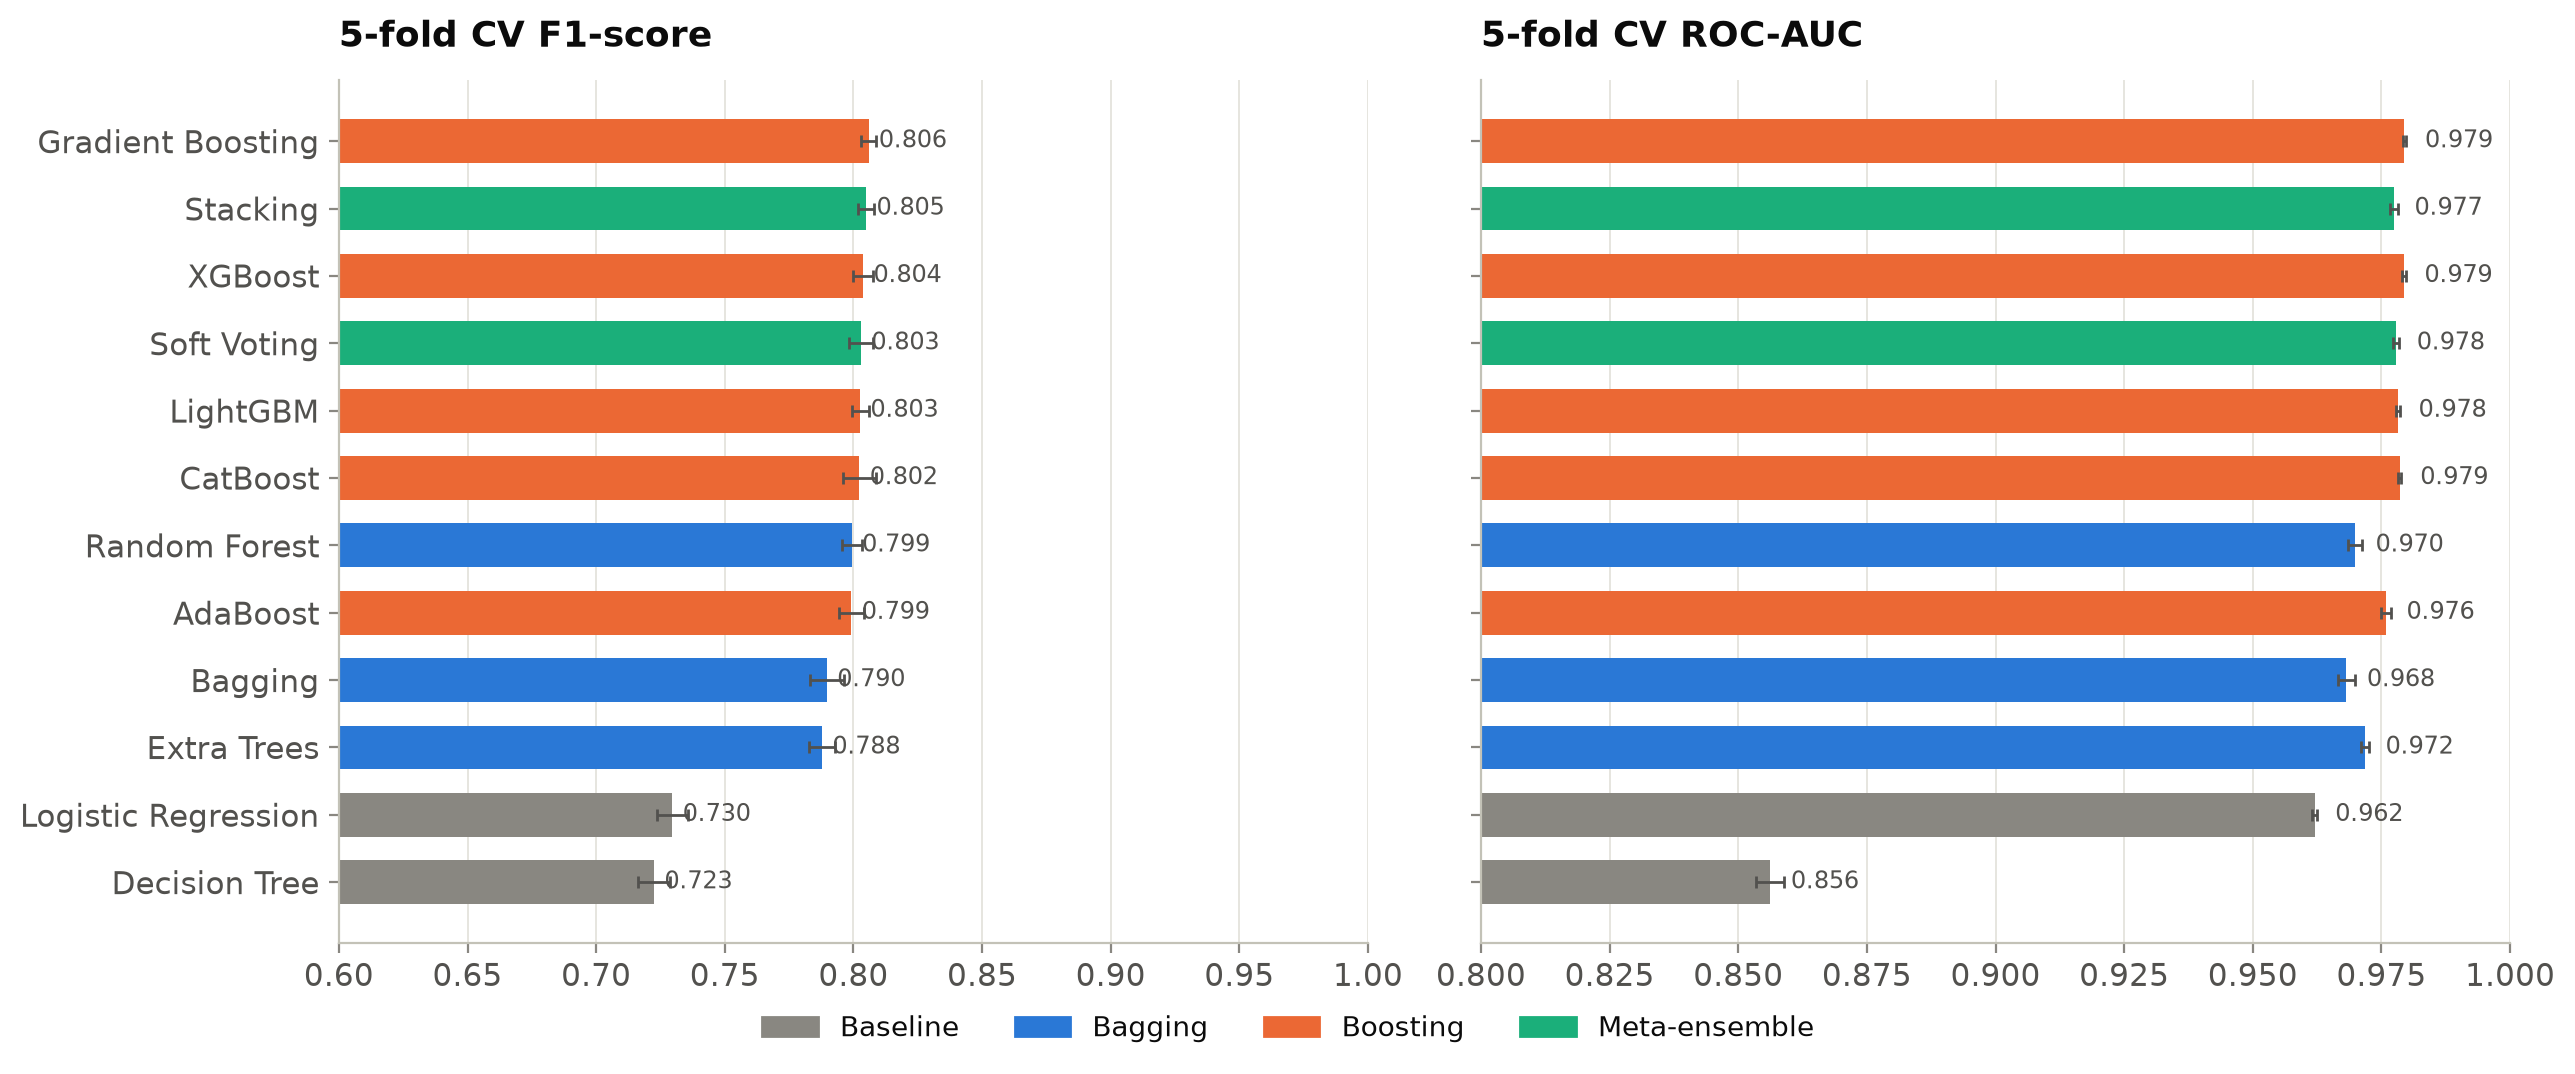
\includegraphics[width=\linewidth]{db_cv_comparison.png}
\caption{5-fold CV F1-score and ROC-AUC with standard deviation (grey = baselines, blue = bagging, orange = boosting, green = meta-ensembles)}
\label{fig:dbcv}
\end{figure}
\textbf{Interpretation (Table~\ref{tab:dbcv}, Figure~\ref{fig:dbcv}).} \DBCVINTERP

\begin{table}[H]
\centering
\caption{Held-out test set results at the default threshold 0.5 (sorted by F1)}
\label{tab:dbtest}
\begin{tabular}{@{}lccccccc@{}}
\toprule
\textbf{Model} & \textbf{Accuracy} & \textbf{Precision} & \textbf{Recall} & \textbf{F1} & \textbf{ROC-AUC} & \textbf{PR-AUC} & \textbf{Fit (s)} \\
\midrule
\dbTestRows
\bottomrule
\end{tabular}
\end{table}
\textbf{Interpretation (Table~\ref{tab:dbtest}).} \DBTESTINTERP

\begin{table}[H]
\centering
\caption{Test results with the F1-optimal threshold chosen on out-of-fold training predictions}
\label{tab:dbthr}
\begin{tabular}{@{}lcccccc@{}}
\toprule
\textbf{Model} & \textbf{Threshold} & \textbf{Accuracy} & \textbf{Precision} & \textbf{Recall} & \textbf{F1} & \textbf{ROC-AUC} \\
\midrule
\dbThrRows
\bottomrule
\end{tabular}
\end{table}
\textbf{Interpretation (Table~\ref{tab:dbthr}).} \DBTHRINTERP

\begin{figure}[H]
\centering
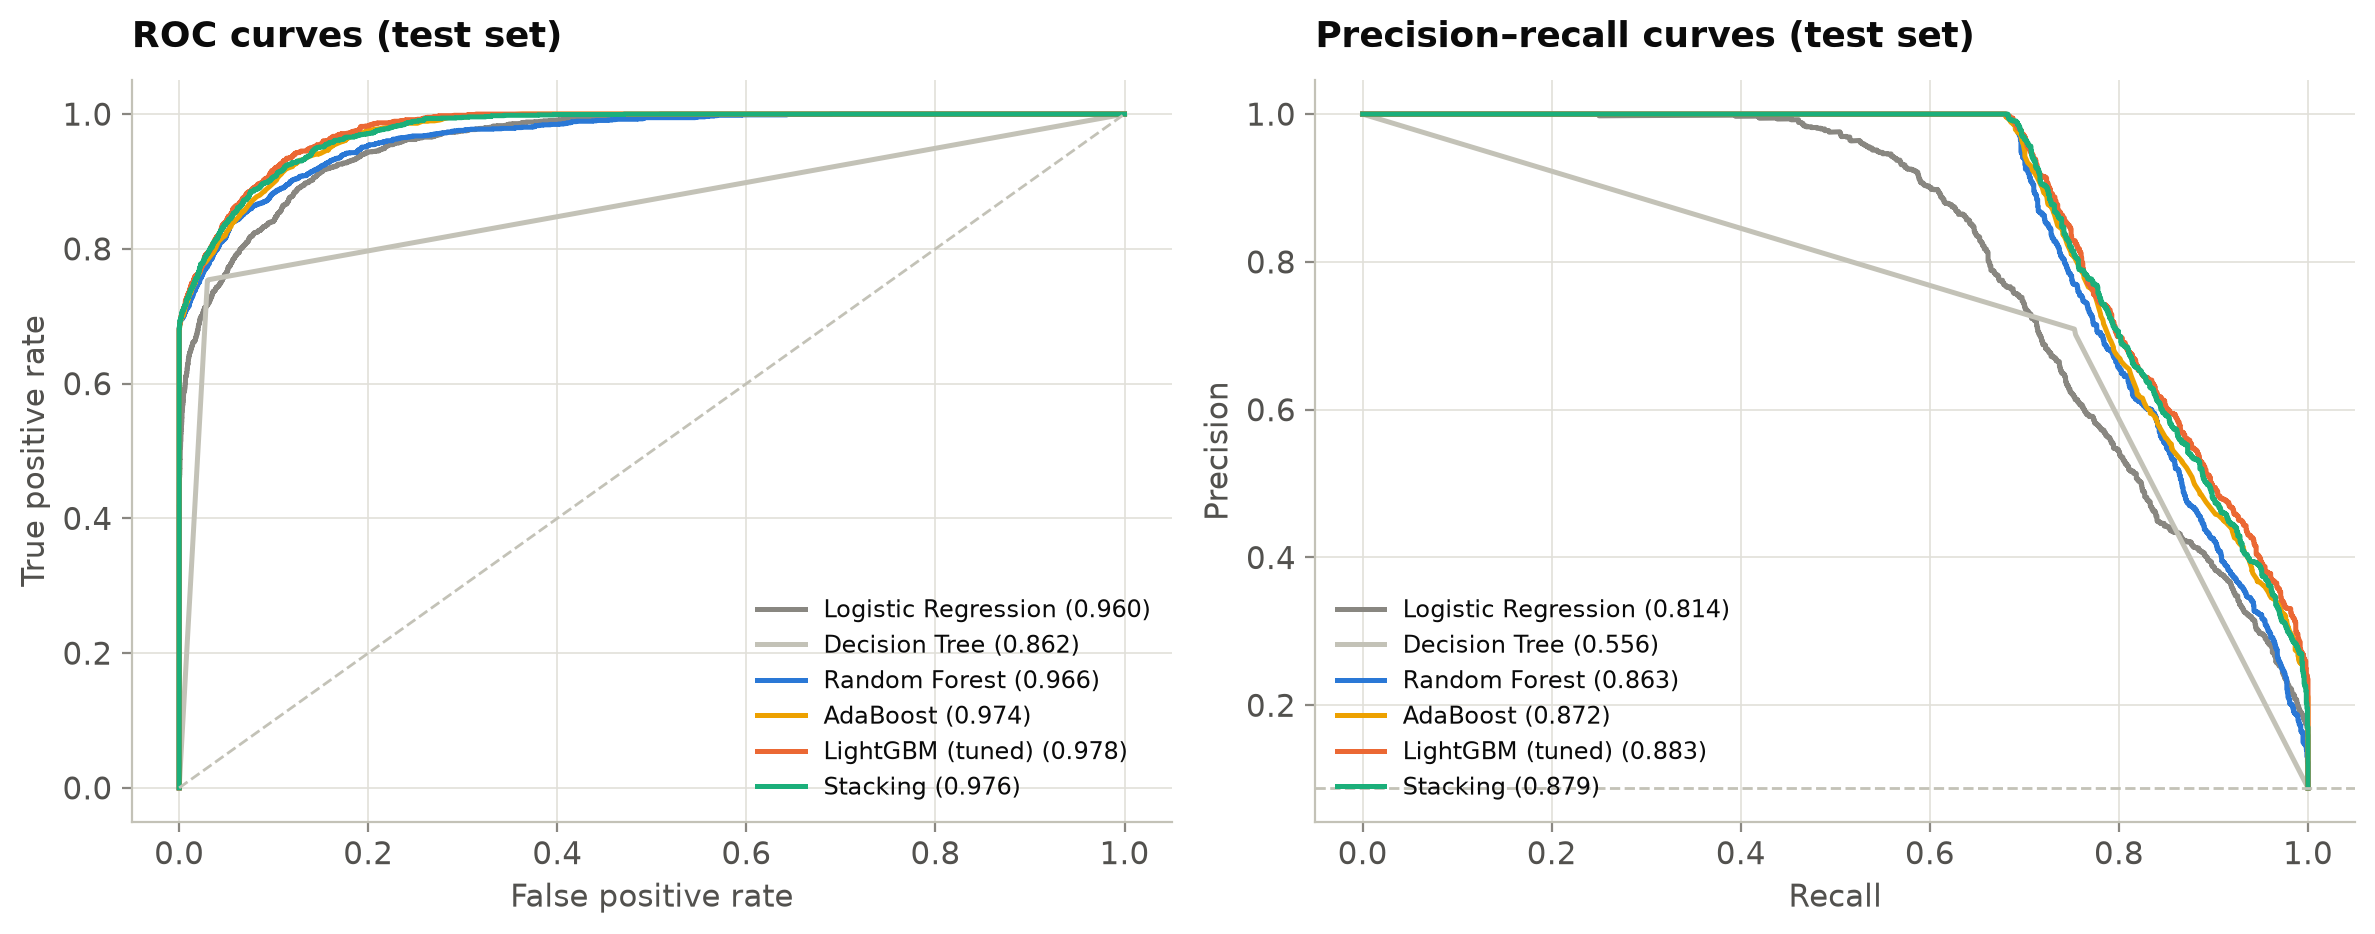
\includegraphics[width=\linewidth]{db_roc_pr.png}
\caption{ROC (left) and precision–recall (right) curves on the test set; AUC values in brackets}
\label{fig:dbroc}
\end{figure}
\textbf{Interpretation (Figure~\ref{fig:dbroc}).} \DBROCINTERP

\begin{figure}[H]
\centering
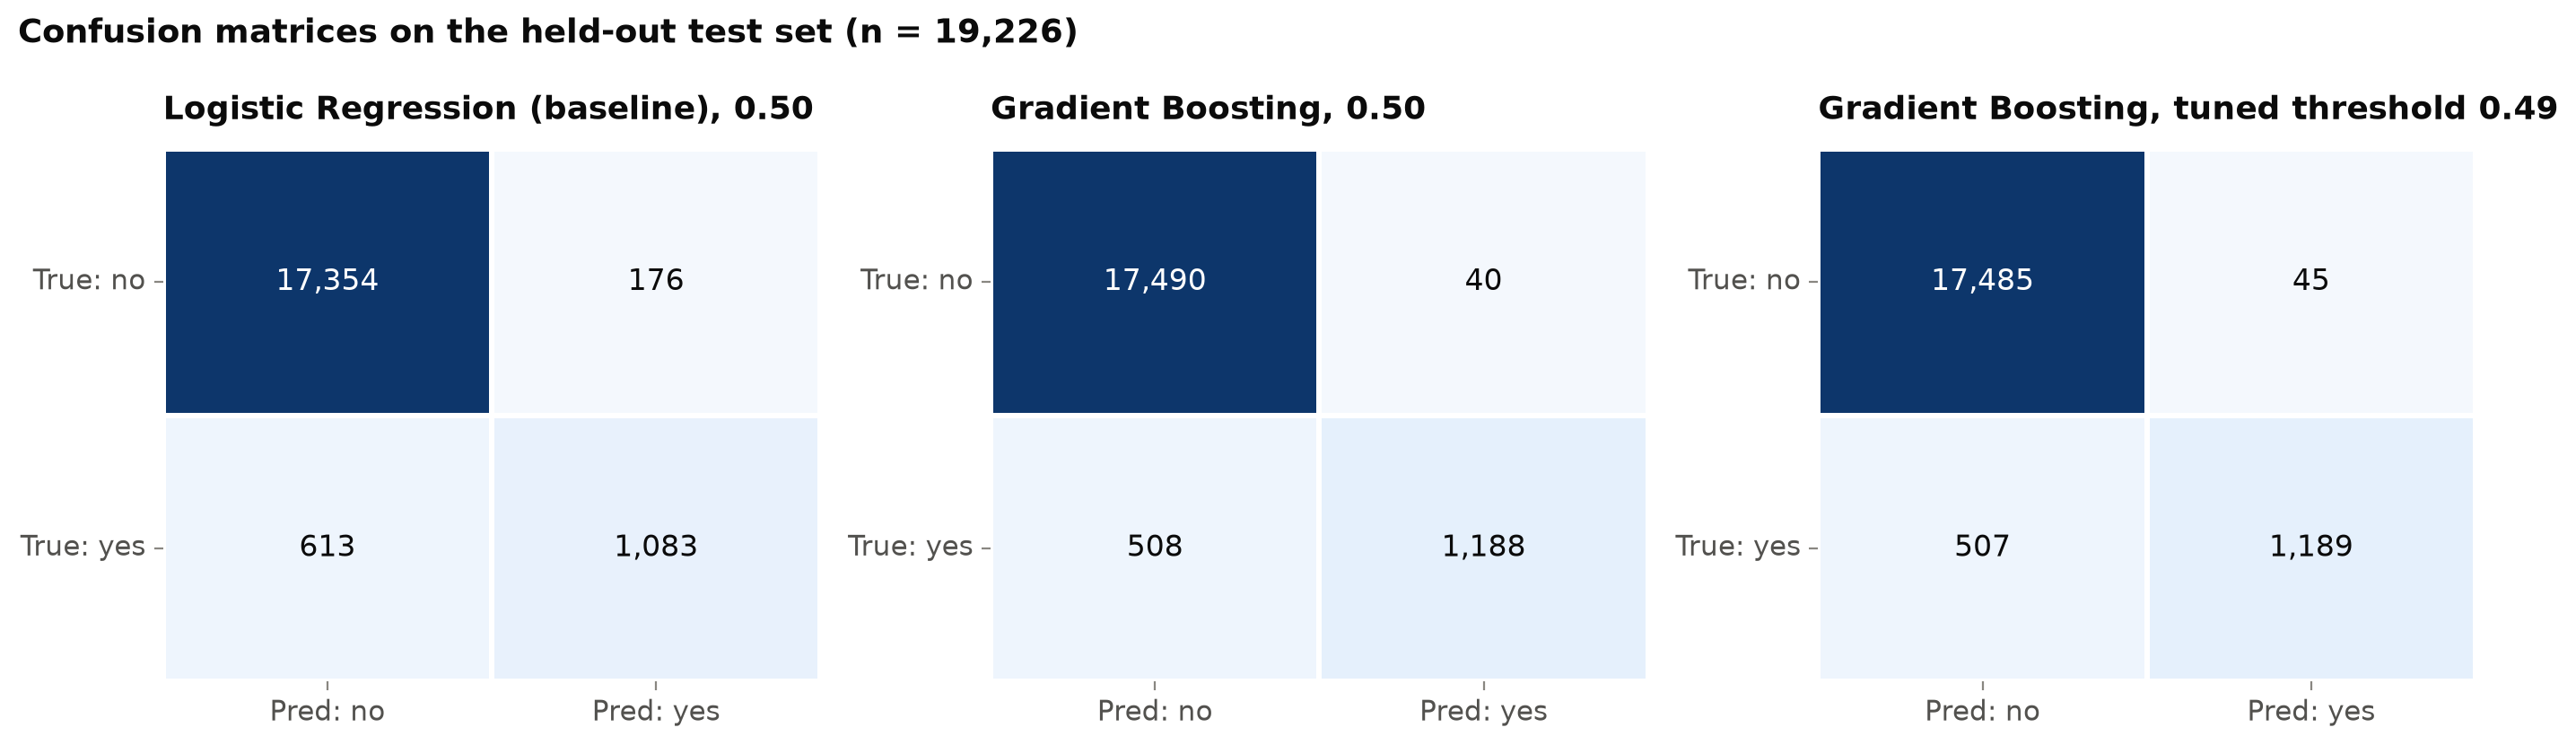
\includegraphics[width=\linewidth]{db_confusion.png}
\caption{Test-set confusion matrices: Logistic Regression baseline, best ensemble at 0.5, and best ensemble at the tuned threshold}
\label{fig:dbcm}
\end{figure}
\textbf{Interpretation (Figure~\ref{fig:dbcm}).} \DBCMINTERP

\begin{figure}[H]
\centering
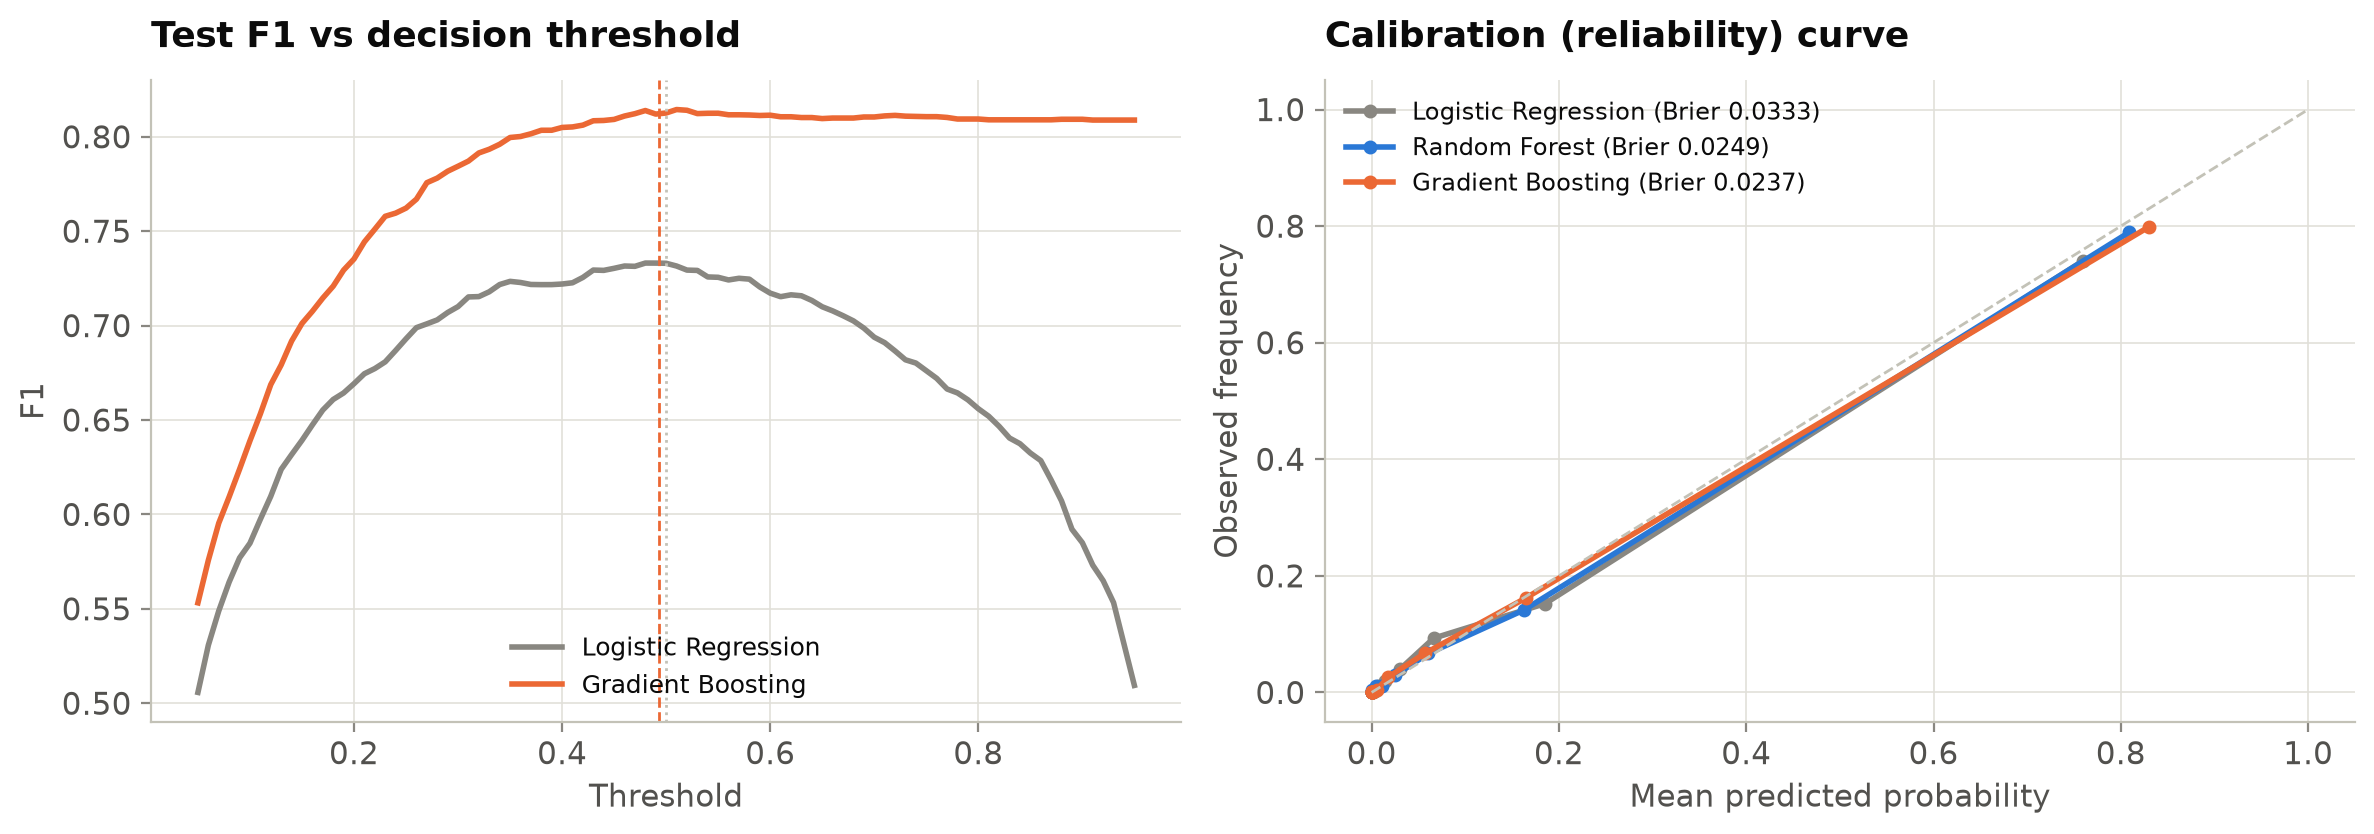
\includegraphics[width=\linewidth]{db_threshold_calibration.png}
\caption{Test F1 as a function of the decision threshold (left) and calibration curves (right)}
\label{fig:dbthr}
\end{figure}
\textbf{Interpretation (Figure~\ref{fig:dbthr}).} \DBTHRCALINTERP

\begin{figure}[H]
\centering
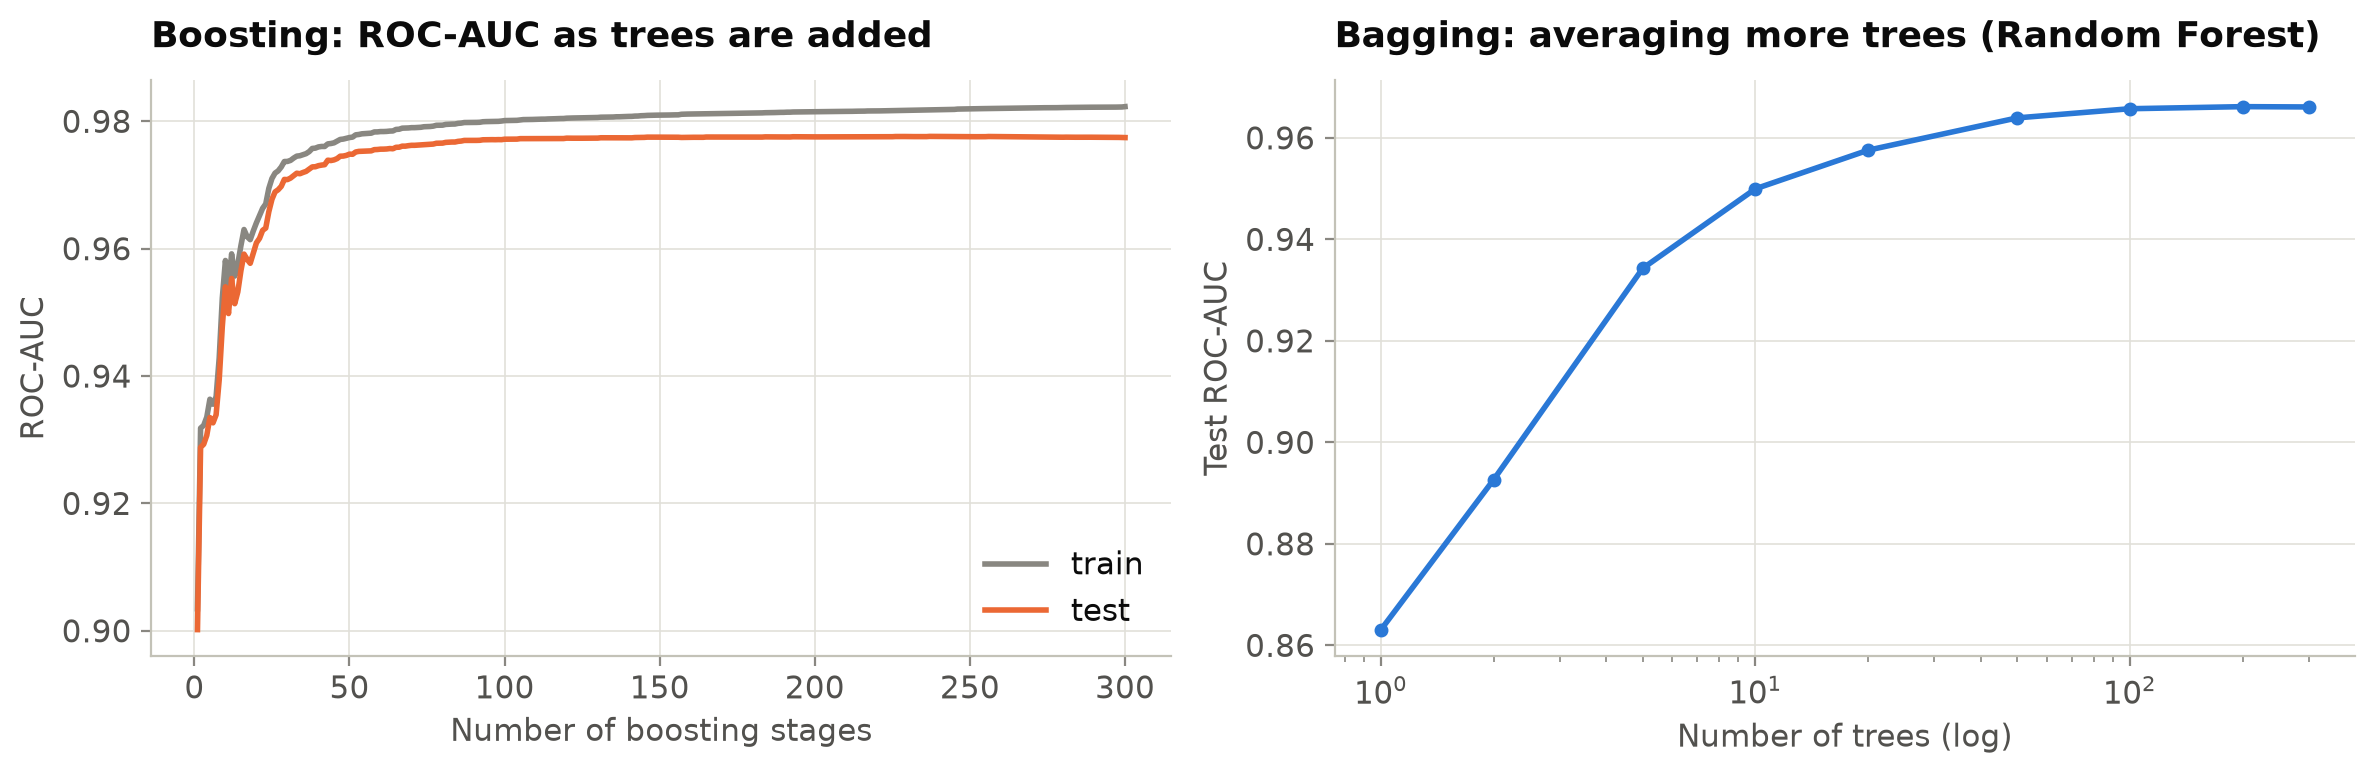
\includegraphics[width=\linewidth]{db_ensemble_size.png}
\caption{How ensembles improve: boosting ROC-AUC as trees are added (left); Random Forest test ROC-AUC vs number of averaged trees (right)}
\label{fig:dbsize}
\end{figure}
\textbf{Interpretation (Figure~\ref{fig:dbsize}).} \DBSIZEINTERP

\begin{table}[H]
\centering
\caption{Statistical significance: paired $t$-test on 5-fold CV F1 against Logistic Regression}
\label{tab:dbsig}
\begin{tabular}{@{}lcc@{}}
\toprule
\textbf{Model} & \textbf{Mean $\Delta$F1 vs LR} & \textbf{$p$-value} \\
\midrule
\dbSigRows
\bottomrule
\end{tabular}
\end{table}
\textbf{Interpretation (Table~\ref{tab:dbsig}).} \DBSIGINTERP

\begin{figure}[H]
\centering
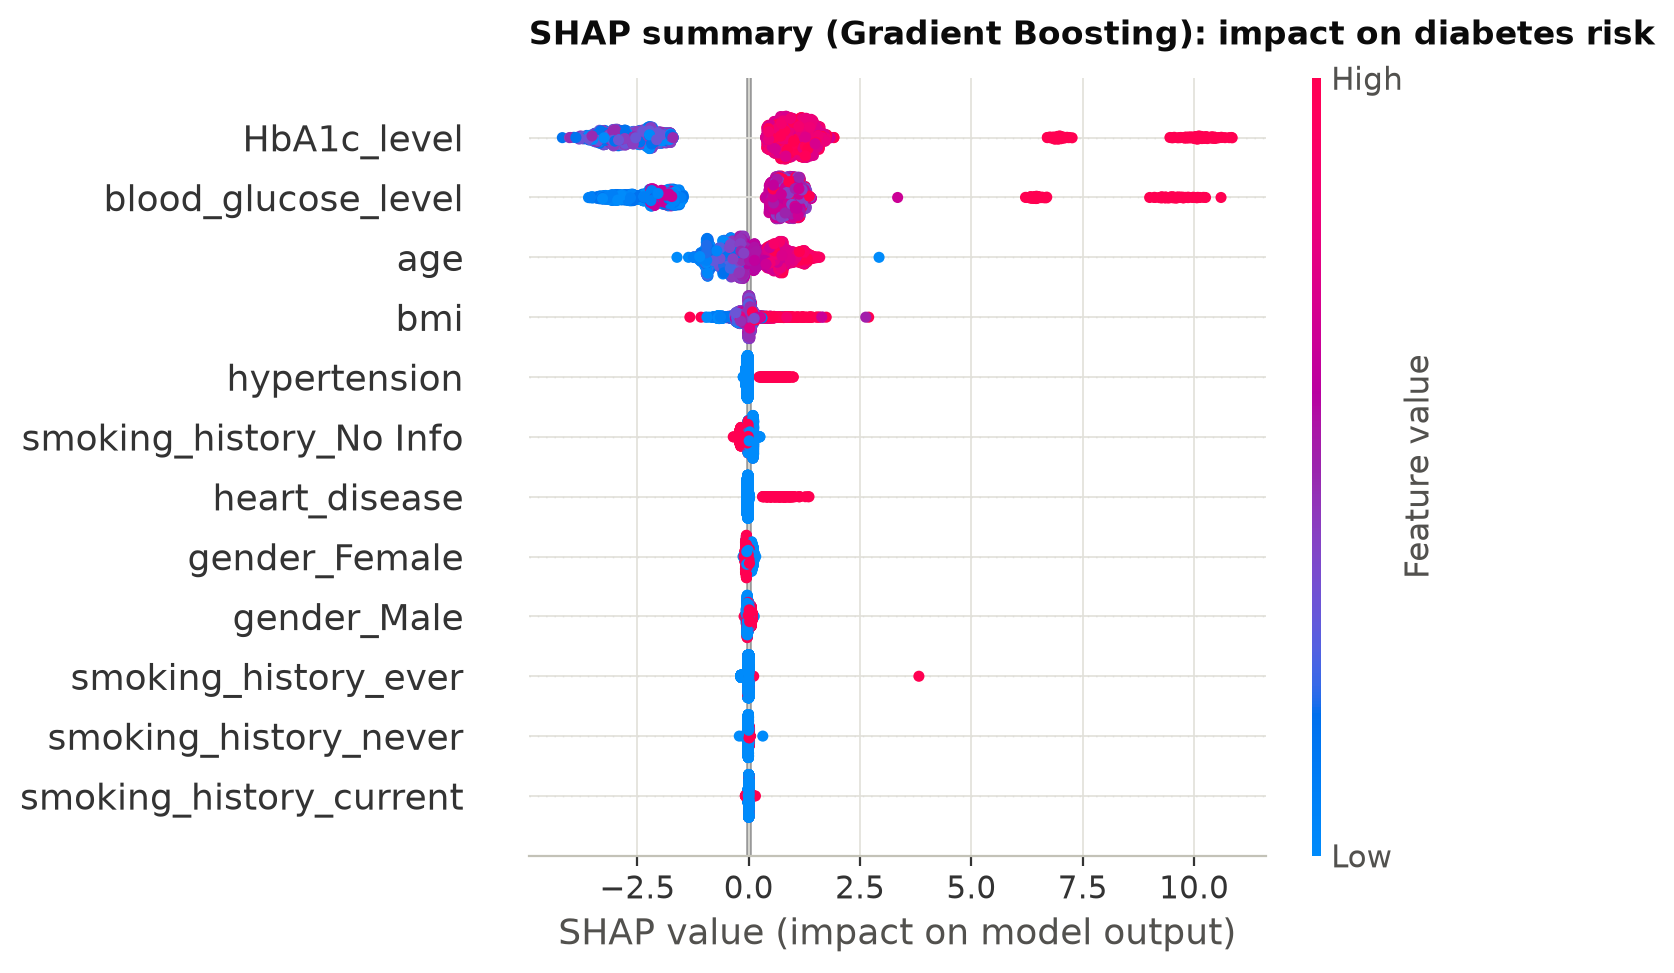
\includegraphics[width=0.56\linewidth]{db_shap_summary.png}\hfill
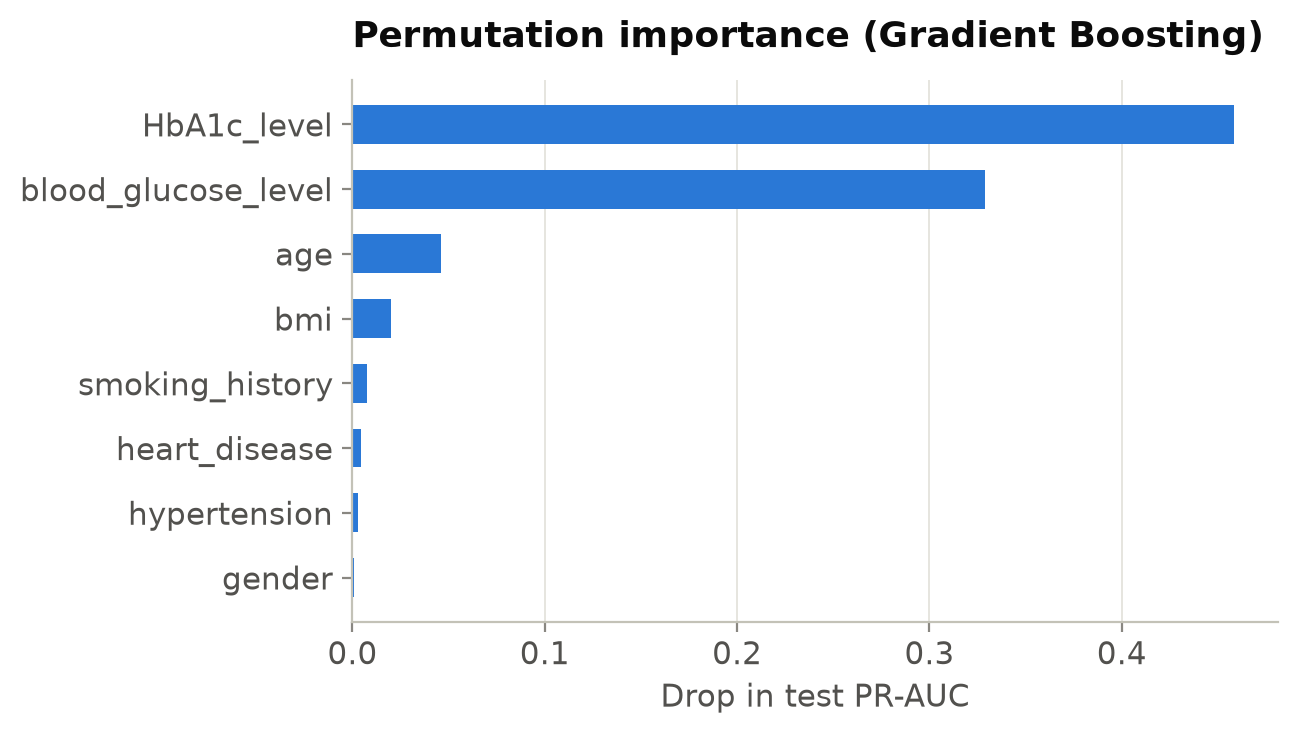
\includegraphics[width=0.42\linewidth]{db_permutation_importance.png}
\caption{SHAP summary for the final \dbShapModel{} model (left) and permutation importance on the test set (right)}
\label{fig:dbshap}
\end{figure}
\begin{figure}[H]
\centering
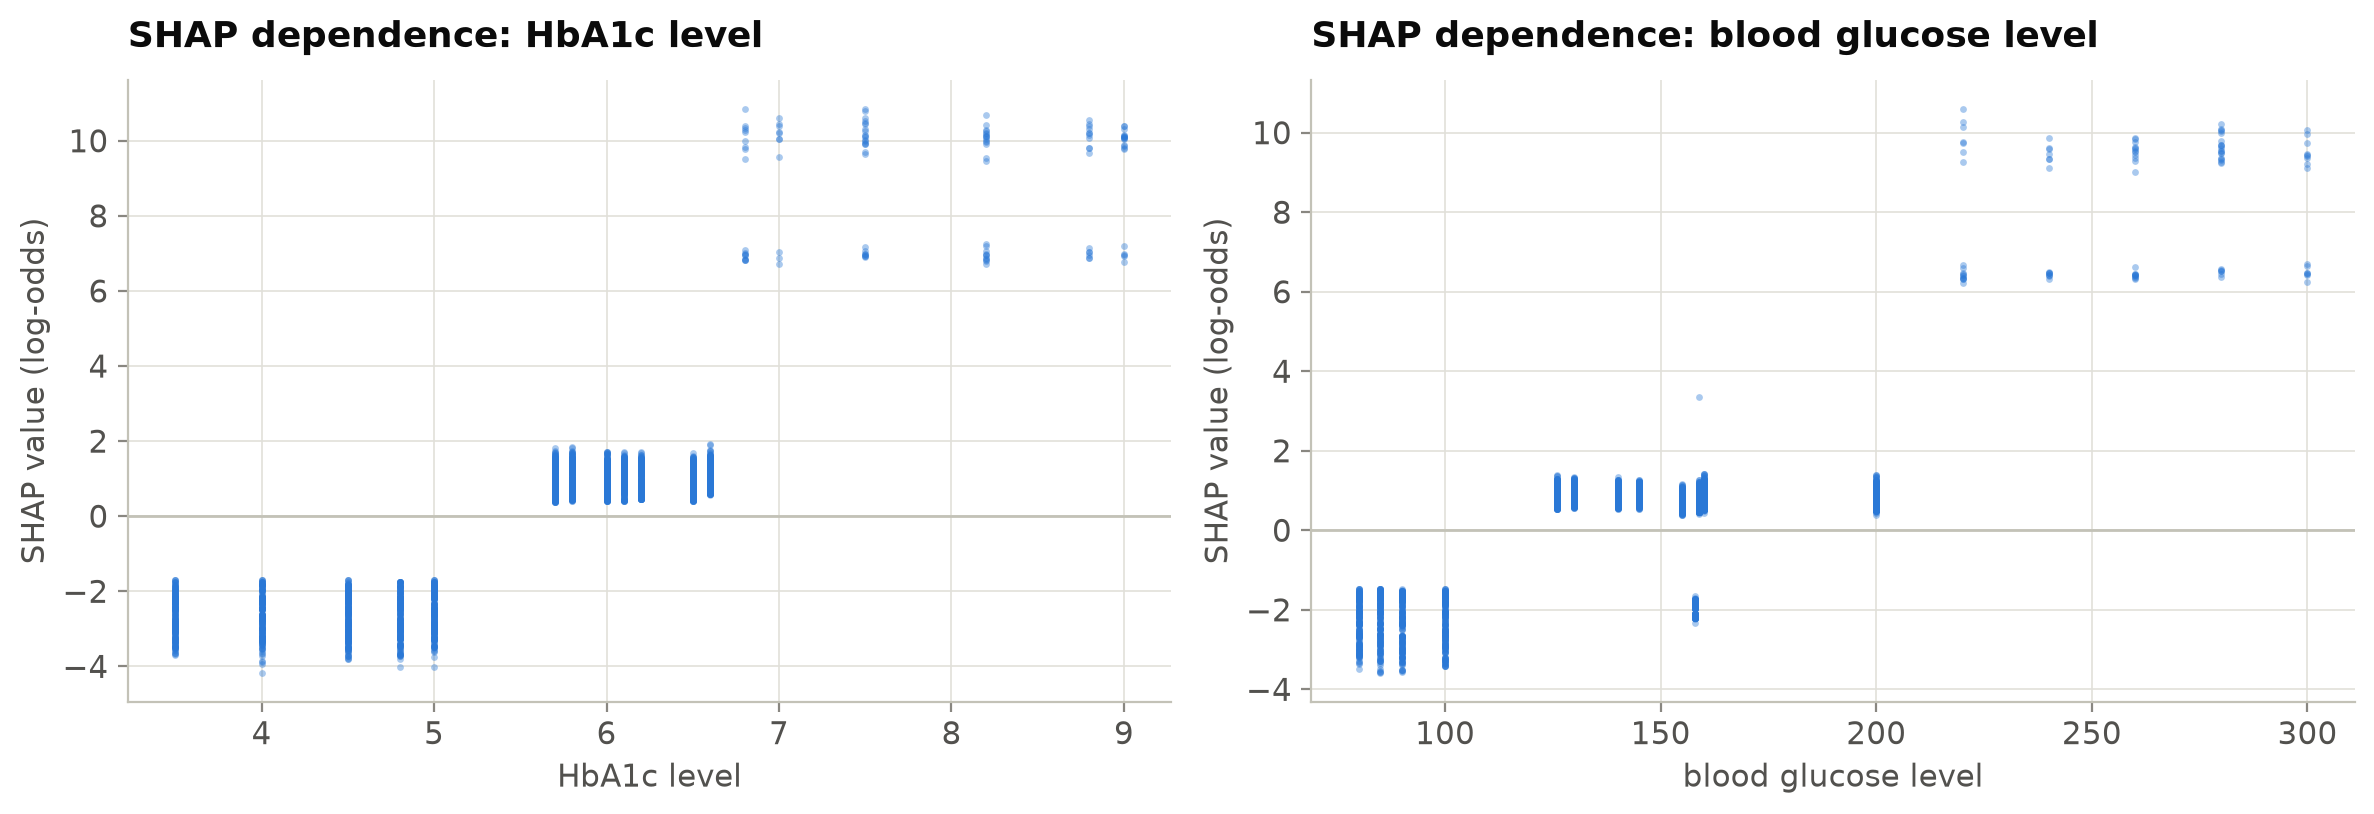
\includegraphics[width=\linewidth]{db_shap_dependence.png}
\caption{SHAP dependence of predicted risk on HbA1c and blood glucose}
\label{fig:dbshapdep}
\end{figure}
\textbf{Interpretation (Figures~\ref{fig:dbshap}–\ref{fig:dbshapdep}).} \DBSHAPINTERP

\section{Comparison with Previous Models}
\DBCOMPARE

\section{Discussion, Findings and Limitations}
\DBDISCUSS

\section{Chapter Conclusion}
\DBCONCL

\chapter{Integrated Discussion and Findings}

This chapter brings together what was learned across PBL I, II and III. Numbers are compared only between models
evaluated on the same task, the same test set and the same metric. Results from different datasets are compared
qualitatively.

\section{Summary of Outcomes per Unit}
\begin{table}[H]
\centering
\caption{Best result of each unit on its own held-out test data}
\label{tab:summary}
\renewcommand{\arraystretch}{1.25}
\begin{tabularx}{\linewidth}{@{}c >{\raggedright\arraybackslash}p{3.3cm} >{\raggedright\arraybackslash}p{3.4cm} >{\raggedright\arraybackslash}X@{}}
\toprule
\textbf{Unit} & \textbf{Task / dataset} & \textbf{Best method} & \textbf{Key result (vs baseline)} \\
\midrule
1 & EDA: Play Store, Video Games & Robust cleaning + rank statistics & Quantified market drivers (e.g.\ reviews–installs $\rho=0.97$; top 1\% of games = 21\% of sales) \\
2 & Regression: CCPP & Tuned XGBoost & RMSE 3.17 MW, $R^2$ 0.966 (linear: 4.59 MW; $-$31\% error) \\
2 & Classification: Bank Marketing & Weighted XGBoost + threshold & F1 0.531, ROC-AUC 0.812, 3.3$\times$ lift (plain LR: F1 0.320) \\
3 & Clustering: UCI HAR & Gaussian Mixture & Accuracy 0.612, ARI 0.486 (K-Means: 0.570) \\
4 & Sequential: UCI HAR & Hybrid HMM + Viterbi & Accuracy 0.987, macro F1 0.988 (same classifier without HMM: 0.964) \\
5 & Ensembles: Diabetes & \dbBestName{} + tuned threshold & F1 \dbBestFone, ROC-AUC \dbBestAuc{} (LR: F1 \dbLrFone, ROC-AUC \dbLrAuc) \\
\bottomrule
\end{tabularx}
\end{table}

\section{Critical Findings Across the Project}
\begin{enumerate}
\item \textbf{Combining many learners beats a single model on tabular data, consistently.} Gradient-boosted tree
ensembles were the best model on every supervised tabular task: CCPP regression (tuned XGBoost), bank-marketing
classification (weighted XGBoost) and diabetes prediction (Chapter 4, where every one of the ten ensembles beat both
baselines on F1 and ROC-AUC). The mechanism is the same in each case. Boosting captures non-linear, interacting effects
that linear models miss, and averaging many trees removes the instability of a single tree.

\item \textbf{The temporal structure adds the same kind of value as an ensemble.} In Unit 4 a strong per-window
classifier made 3.6\% errors. Adding a Markov chain and decoding with Viterbi removed 63\% of them, because each
prediction is combined with the evidence from neighbouring windows. Like an ensemble, the HMM pools evidence to correct
isolated mistakes; here the pooling runs over time rather than over models.

\item \textbf{The right metric matters more than the model when classes are imbalanced.} Three datasets were
imbalanced: bank 11.3\% positive, diabetes 8.8\%, and the activity classes once sequences are considered. On each, a
trivial or plain model reached high accuracy while missing most positives (bank: 89.8\% accuracy with only 21\% recall).
Evaluating with F1, recall, ROC-AUC and PR-AUC, and choosing the decision threshold on out-of-fold training predictions,
consistently gave more useful models: bank F1 0.487 $\rightarrow$ 0.531, and a similar threshold gain for diabetes
(Chapter 4).

\item \textbf{Leakage control is essential for honest results.} Each review had its own leakage risk: the
\texttt{duration} feature in the bank data, duplicate patient records in the diabetes data, and person overlap in HAR.
Each was removed or controlled (feature dropped, duplicates removed before splitting, split by subject). Preprocessing
and model selection always ran inside training folds.

\item \textbf{Unsupervised structure is not the same as semantic labels.} K-Means clusters of HAR windows were
geometrically \emph{tighter} than the true activities (silhouette 0.41 vs 0.26) yet matched them only 57\% of the time.
Unsupervised methods reveal how data is organised, which is valuable for exploration, but they do not replace labels
when a specific target matters.

\item \textbf{Interpretation confirms domain knowledge.} Permutation importance and SHAP identified ambient temperature
as the driver of power output, past campaign success and the macro-economy as drivers of subscription, and HbA1c,
glucose, age and BMI as drivers of diabetes risk. In each case the model's explanations matched the physics, the
marketing literature or clinical guidelines, which increases trust in the models.
\end{enumerate}

\section{Comparability of Results}
Only models on the same dataset, split and metric are compared numerically: the rows of each table in Chapters 2–4.
The six summary rows of Table~\ref{tab:summary} come from different datasets with different difficulty and class
balance. For example, the diabetes F1 (\dbBestFone) and the bank F1 (0.531) should not be read as ``the diabetes model is
better''. The diabetes data contains much stronger predictors (HbA1c and glucose), while the bank data is limited to
information available before a call.

\section{Study Limitations}
\begin{itemize}
\item \textbf{Different datasets per unit.} The allotted topics used different datasets, so the five units cannot be
evaluated on one common benchmark.
\item \textbf{Public, curated data.} All datasets are public snapshots: laboratory HAR recordings, a 2008–2010 bank
campaign, and a curated diabetes dataset whose laboratory values are recorded at a few discrete levels. Performance on
raw clinical or field data is likely to be lower.
\item \textbf{Tuning budget.} Only the leading family in each task was tuned extensively; the other models used
sensible defaults.
\item \textbf{No external validation.} Each model was validated on a held-out split of the same source, not on an
independent cohort or site.
\end{itemize}

\chapter{Overall Conclusion and Future Scope}

\section{Conclusion}
This project designed, implemented and rigorously evaluated machine-learning pipelines across all five units of the
course. Every result was measured on held-out data.
\begin{itemize}
\item \textbf{Unit 1:} cleaning and exploratory analysis turned two messy market datasets into quantified insights.
Free apps dominate installs (92.2\% of apps; median 100,000 vs 1,000 installs for paid apps). Video-game sales are
concentrated in hits (the top 1\% of titles earn 21.1\% of sales) and peaked in 2008.
\item \textbf{Unit 2:} tuned XGBoost predicted power-plant output with RMSE 3.17 MW ($R^2$ 0.966), 31\% lower error than
linear regression. An imbalance-aware, leakage-free XGBoost model identified bank-deposit subscribers with F1 0.531 and
a 3.3$\times$ lift over random calling.
\item \textbf{Unit 3:} K-Means and Gaussian Mixture clustering recovered the static/dynamic structure of smartphone
activity data (accuracy up to 0.612 without labels), and showed that geometric clusters differ from semantic activities.
\item \textbf{Unit 4:} the forward–backward and Viterbi algorithms were implemented from first principles and verified
against \texttt{hmmlearn} (difference $<10^{-9}$). A supervised hybrid HMM decoded the activity sequences of unseen
people with 98.7\% accuracy; its Markov chain removed 63\% of the per-window errors.
\item \textbf{Unit 5:} ten ensemble classifiers were implemented and compared with Logistic Regression and Decision Tree
baselines for diabetes prediction. The best model, \dbBestName{} with an out-of-fold-tuned threshold, reached
\textbf{F1 \dbBestFone{} and ROC-AUC \dbBestAuc{}} (accuracy \dbBestAccPct) on \dbTest{} unseen patients, against F1
\dbLrFone{} for Logistic Regression and \dbDtFone{} for the Decision Tree. The improvement is statistically significant,
and SHAP explanations agree with clinical guidelines.
\end{itemize}
The central lesson is that good machine learning depends as much on \emph{methodology} as on algorithms. The methodology
used throughout was: careful cleaning, leakage control, metrics matched to the class balance, cross-validated model
selection, thresholds chosen on training data, and interpretation. Within that methodology, combining learners, whether
over models (ensembles) or over time (HMMs), consistently gave the most accurate and reliable predictions.

\section{Future Scope}
\begin{enumerate}
\item \textbf{External and prospective validation:} test the diabetes model on an independent hospital cohort with raw,
continuous laboratory values, and the HAR model on free-living data with different phone positions.
\item \textbf{Cost-sensitive decisions:} replace F1-optimal thresholds with thresholds derived from real costs (e.g.\ the
cost of a missed diabetic vs an unnecessary test, or of a call vs a deposit).
\item \textbf{Broader tuning:} Bayesian optimisation (e.g.\ Optuna) for all leading models, and weighted or
learned-weight voting ensembles.
\item \textbf{Richer sequential models:} semi-supervised HMMs that need only a few labels, hidden semi-Markov models with
explicit activity durations, and neural sequence models for comparison.
\item \textbf{Deployment and interpretability:} package the diabetes model as a web-based risk calculator that shows
per-patient SHAP explanations to clinicians, with monitoring for data drift.
\item \textbf{Fairness:} audit model performance across gender and age groups before any clinical use.
\end{enumerate}

\clearpage
\phantomsection
\addcontentsline{toc}{chapter}{REFERENCES}
\renewcommand{\bibname}{REFERENCES}
\begin{singlespace}
\begin{thebibliography}{99}
\setlength{\itemsep}{4pt}
\fontsize{11.5}{14}\selectfont

\bibitem{miotto} R. Miotto, L. Wang, S. Wang, X. Jiang, and J. T. Dudley, ``Deep learning for healthcare: review, opportunities and challenges,'' \emph{Briefings in Bioinformatics}, vol. 19, no. 6, pp. 1236–1246, 2018.
\bibitem{ada} American Diabetes Association Professional Practice Committee, ``2. Diagnosis and classification of diabetes: Standards of Care in Diabetes—2024,'' \emph{Diabetes Care}, vol. 47, suppl. 1, pp. S20–S42, 2024.
\bibitem{diabdata} M. Mustafa, ``Diabetes Prediction Dataset,'' Kaggle, 2023. [Online]. Available: \url{https://www.kaggle.com/datasets/iammustafatz/diabetes-prediction-dataset}
\bibitem{breiman96} L. Breiman, ``Bagging predictors,'' \emph{Machine Learning}, vol. 24, no. 2, pp. 123–140, 1996.
\bibitem{breiman01} L. Breiman, ``Random forests,'' \emph{Machine Learning}, vol. 45, no. 1, pp. 5–32, 2001.
\bibitem{geurts} P. Geurts, D. Ernst, and L. Wehenkel, ``Extremely randomized trees,'' \emph{Machine Learning}, vol. 63, no. 1, pp. 3–42, 2006.
\bibitem{freund} Y. Freund and R. E. Schapire, ``A decision-theoretic generalization of on-line learning and an application to boosting,'' \emph{Journal of Computer and System Sciences}, vol. 55, no. 1, pp. 119–139, 1997.
\bibitem{friedman} J. H. Friedman, ``Greedy function approximation: A gradient boosting machine,'' \emph{The Annals of Statistics}, vol. 29, no. 5, pp. 1189–1232, 2001.
\bibitem{xgboost} T. Chen and C. Guestrin, ``XGBoost: A scalable tree boosting system,'' in \emph{Proc. 22nd ACM SIGKDD Int. Conf. Knowledge Discovery and Data Mining}, 2016, pp. 785–794.
\bibitem{lightgbm} G. Ke \emph{et al.}, ``LightGBM: A highly efficient gradient boosting decision tree,'' in \emph{Advances in Neural Information Processing Systems 30}, 2017, pp. 3146–3154.
\bibitem{catboost} L. Prokhorenkova, G. Gusev, A. Vorobev, A. V. Dorogush, and A. Gulin, ``CatBoost: unbiased boosting with categorical features,'' in \emph{Advances in Neural Information Processing Systems 31}, 2018, pp. 6638–6648.
\bibitem{wolpert} D. H. Wolpert, ``Stacked generalization,'' \emph{Neural Networks}, vol. 5, no. 2, pp. 241–259, 1992.
\bibitem{shap} S. M. Lundberg and S.-I. Lee, ``A unified approach to interpreting model predictions,'' in \emph{Advances in Neural Information Processing Systems 30}, 2017, pp. 4765–4774.
\bibitem{mcnemar} Q. McNemar, ``Note on the sampling error of the difference between correlated proportions or percentages,'' \emph{Psychometrika}, vol. 12, no. 2, pp. 153–157, 1947.
\bibitem{rabiner} L. R. Rabiner, ``A tutorial on hidden Markov models and selected applications in speech recognition,'' \emph{Proceedings of the IEEE}, vol. 77, no. 2, pp. 257–286, 1989.
\bibitem{viterbi} A. J. Viterbi, ``Error bounds for convolutional codes and an asymptotically optimum decoding algorithm,'' \emph{IEEE Trans. Information Theory}, vol. 13, no. 2, pp. 260–269, 1967.
\bibitem{baum} L. E. Baum, T. Petrie, G. Soules, and N. Weiss, ``A maximization technique occurring in the statistical analysis of probabilistic functions of Markov chains,'' \emph{The Annals of Mathematical Statistics}, vol. 41, no. 1, pp. 164–171, 1970.
\bibitem{bourlard} H. A. Bourlard and N. Morgan, \emph{Connectionist Speech Recognition: A Hybrid Approach}. Boston, MA, USA: Kluwer Academic, 1994.
\bibitem{dempster} A. P. Dempster, N. M. Laird, and D. B. Rubin, ``Maximum likelihood from incomplete data via the EM algorithm,'' \emph{Journal of the Royal Statistical Society, Series B}, vol. 39, no. 1, pp. 1–38, 1977.
\bibitem{lloyd} S. P. Lloyd, ``Least squares quantization in PCM,'' \emph{IEEE Trans. Information Theory}, vol. 28, no. 2, pp. 129–137, 1982.
\bibitem{kuhn} H. W. Kuhn, ``The Hungarian method for the assignment problem,'' \emph{Naval Research Logistics Quarterly}, vol. 2, no. 1–2, pp. 83–97, 1955.
\bibitem{anguita} D. Anguita, A. Ghio, L. Oneto, X. Parra, and J. L. Reyes-Ortiz, ``A public domain dataset for human activity recognition using smartphones,'' in \emph{Proc. 21st European Symposium on Artificial Neural Networks (ESANN)}, Bruges, Belgium, 2013, pp. 437–442.
\bibitem{tufekci} P. Tüfekci, ``Prediction of full load electrical power output of a base load operated combined cycle power plant using machine learning methods,'' \emph{Int. J. Electrical Power \& Energy Systems}, vol. 60, pp. 126–140, 2014.
\bibitem{moro} S. Moro, P. Cortez, and P. Rita, ``A data-driven approach to predict the success of bank telemarketing,'' \emph{Decision Support Systems}, vol. 62, pp. 22–31, 2014.
\bibitem{chawla} N. V. Chawla, K. W. Bowyer, L. O. Hall, and W. P. Kegelmeyer, ``SMOTE: Synthetic minority over-sampling technique,'' \emph{Journal of Artificial Intelligence Research}, vol. 16, pp. 321–357, 2002.
\bibitem{sklearn} F. Pedregosa \emph{et al.}, ``Scikit-learn: Machine learning in Python,'' \emph{Journal of Machine Learning Research}, vol. 12, pp. 2825–2830, 2011.
\bibitem{esl} T. Hastie, R. Tibshirani, and J. Friedman, \emph{The Elements of Statistical Learning}, 2nd ed. New York, NY, USA: Springer, 2009.
\bibitem{murphy} K. P. Murphy, \emph{Machine Learning: A Probabilistic Perspective}. Cambridge, MA, USA: MIT Press, 2012.
\bibitem{playstore} L. Gupta, ``Google Play Store Apps,'' Kaggle, 2019. [Online]. Available: \url{https://www.kaggle.com/datasets/lava18/google-play-store-apps}
\bibitem{vgsales} G. Smith, ``Video Game Sales,'' Kaggle, 2016. [Online]. Available: \url{https://www.kaggle.com/datasets/gregorut/videogamesales}
\end{thebibliography}
\end{singlespace}

\clearpage
\phantomsection
\addcontentsline{toc}{chapter}{APPENDIX A – CODING}
\begin{center}{\bfseries\fontsize{16}{20}\selectfont APPENDIX A\\[4pt] CODING}\end{center}
\vspace{6pt}
All code is written in Python 3.13 with pandas, scikit-learn, XGBoost, LightGBM, CatBoost, imbalanced-learn, hmmlearn,
SHAP, statsmodels, matplotlib and seaborn. Every notebook is self-contained and runs top to bottom in Google Colab; the
dataset download is included. All randomness is fixed with \texttt{random\_state = 42}, so the numbers in this report
are reproducible. The listings below contain the complete code cells of each notebook.

\renewcommand{\arraystretch}{1.25}
\begin{table}[H]
\centering
\caption{Notebooks and Google Colab links}
\label{tab:colab}
\begin{tabularx}{\linewidth}{@{}l l >{\raggedright\arraybackslash}X@{}}
\toprule
\textbf{Unit} & \textbf{Notebook} & \textbf{Google Colab link} \\
\midrule
1 & \texttt{01\_eda\_play\_store.ipynb} & \colabA \\
1 & \texttt{02\_eda\_video\_game\_sales.ipynb} & \colabB \\
2 & \texttt{03\_regression\_ccpp.ipynb} & \colabC \\
2 & \texttt{04\_classification\_bank\_marketing.ipynb} & \colabD \\
3–4 & \texttt{07\_eda\_har\_accelerometer.ipynb} & \colabE \\
3–4 & \texttt{08\_hmm\_activity\_recognition.ipynb} & \colabF \\
5 & \texttt{09\_diabetes\_ensembles.ipynb} & \colabG \\
\bottomrule
\end{tabularx}
\end{table}

\section*{Chapter 2 – Implementation Methodology and Algorithm Configuration}
\addcontentsline{toc}{section}{Chapter 2 – Implementation Methodology and Algorithm Configuration}
Shared plotting helpers (\texttt{src/viz.py}), followed by the Unit 1 EDA notebooks and the Unit 2 regression and
classification notebooks. Key configurations: 80/20 split, 5-fold (stratified) CV, XGBoost grid search (16
configurations), class weighting / SMOTE, and an F1-optimal threshold chosen on out-of-fold predictions.

\subsection*{A.1 Shared helpers – \texttt{src/viz.py}}
\lstinputlisting{code/viz.py}
\subsection*{A.2 Unit 1 – Play Store EDA (\texttt{01\_eda\_play\_store})}
\lstinputlisting{code/01_eda_play_store.py}
\subsection*{A.3 Unit 1 – Video Game Sales EDA (\texttt{02\_eda\_video\_game\_sales})}
\lstinputlisting{code/02_eda_video_game_sales.py}
\subsection*{A.4 Unit 2 – CCPP Regression (\texttt{03\_regression\_ccpp})}
\lstinputlisting{code/03_regression_ccpp.py}
\subsection*{A.5 Unit 2 – Bank Marketing Classification (\texttt{04\_classification\_bank\_marketing})}
\lstinputlisting{code/04_classification_bank_marketing.py}

\section*{Chapter 3 – Unit 3: Proposed Workflow and Implementation Methodology}
\addcontentsline{toc}{section}{Chapter 3 – Unit 3: Proposed Workflow and Implementation Methodology}
HAR data loading, windowing and feature engineering (notebook 07). The K-Means and GMM clustering with Hungarian
matching and PCA visualisation are in Section 6 of notebook 08 below.
\subsection*{A.6 Units 3–4 – HAR EDA and Features (\texttt{07\_eda\_har\_accelerometer})}
\lstinputlisting{code/07_eda_har_accelerometer.py}

\section*{Chapter 3 – Unit 4: Proposed Workflow and Implementation Methodology}
\addcontentsline{toc}{section}{Chapter 3 – Unit 4: Proposed Workflow and Implementation Methodology}
Unsupervised Gaussian HMM (6 states, full covariance, Baum–Welch, 8 restarts), the hand-coded forward–backward and
Viterbi algorithms with verification, the clustering baselines, and the supervised hybrid HMM (561 features, counted
transition matrix, log-space Viterbi and forward–backward).
\subsection*{A.7 Units 3–4 – HMM, Clustering and Supervised HMM (\texttt{08\_hmm\_activity\_recognition})}
\lstinputlisting{code/08_hmm_activity_recognition.py}

\section*{Chapter 4 – Implementation Methodology and Hyperparameter Configuration}
\addcontentsline{toc}{section}{Chapter 4 – Implementation Methodology and Hyperparameter Configuration}
Diabetes prediction: cleaning, EDA, 2 baselines and 10 ensembles, 5-fold stratified CV, test evaluation, LightGBM
randomised search (40 configurations $\times$ 5 folds, PR-AUC), out-of-fold threshold optimisation, significance tests
and SHAP interpretation. The tuned LightGBM hyperparameters are listed in Table~\ref{tab:tuned}.
\subsection*{A.8 Unit 5 – Ensemble Learning for Diabetes Prediction (\texttt{09\_diabetes\_ensembles})}
\lstinputlisting{code/09_diabetes_ensembles.py}


\end{document}
